\documentclass{article}
\usepackage{anyfontsize} % 消除字体差距报错
\usepackage[UTF8]{ctex}
\usepackage[english]{babel}
\usepackage{hyperref}
\usepackage{amsmath}
\usepackage{mathabx}
\usepackage{lmodern} % 消除字体差距引起的报错
\usepackage{bookmark}
\usepackage{xcolor}
\usepackage{amsthm}
\usepackage{float}
\usepackage{listings}
\usepackage{geometry}
\usepackage{graphicx}
\usepackage{listings}
\usepackage[dvipsnames]{xcolor}
\lstset{
    language=c,
    % basicstyle=\ttfamily, % 设置字体族
    breaklines=true,
    keywordstyle=\bfseries\color{NavyBlue}, % 设置关键字为粗体,颜色为 NavyBlue
    % morekeywords={}, % 设置更多的关键字,用逗号分隔
    % emph={self}, % 指定强调词,如果有多个,用逗号隔开
    % emphstyle=\bfseries\color{Rhodamine}, % 强调词样式设置
    commentstyle=\itshape\color{black!50!white}, % 设置注释样式,斜体,浅灰色
    stringstyle=\bfseries\color{PineGreen!90!black}, % 设置字符串样式
    columns=flexible,
    numbers=left, % 显示行号在左边
    numbersep=2em, % 设置行号的具体位置
    numberstyle=\footnotesize, % 缩小行号
    frame=single, % 边框
    framesep=0.5em % 设置代码与边框的距离
}
\geometry{
    a4paper, % 设置纸张大小为A4
    total={170mm,257mm}, % 设置页面总宽度为170mm,总高度为257mm
    left=20mm, % 设置左边距为20mm
    top=20mm % 设置上边距为20mm
}
\newtheorem*{Definition}{Definition}
\newtheorem*{Theorem}{Theorem}
\newtheorem*{Lemma}{Lemma}
\newtheorem*{Tips}{Tips}
\newtheorem*{Exercise}{Exercise}
\hypersetup{hidelinks,
    colorlinks=true,
    allcolors=black,
    pdfstartview=Fit,
    breaklinks=true}
\author{Melody}
\title{ADS learning}
\begin{document}

\maketitle
\tableofcontents
\newpage

\section{AVL Tree}
\hypertarget{AVL}{}

\begin{itemize}
    \item [\textbf{Target}] Speed up searching (with insertion and deletion). 
    \item [\textbf{Tool}] Binary search trees. 
    \item [\textbf{Problem}] Although $T_p=O(height)$, but the height can be as bad as $O(N)$. 
\end{itemize}

\begin{Tips}
    \item \textbf{height}(该节点往下)\par
    The height of a node is the number of edges on the longest path from the node to a leaf.\par
    \textbf{attention:} the height of an empty tree is defined to be -1.
    \item \textbf{depth}(该节点往上)\par
    The depth of a node is the number of edges from the root to the node.
\end{Tips}

\subsection{definition}
An empty binary tree is height balanced. If $T$ is a nonempty binary tree with $T_L$ and $T_R$ as its left and right subtrees, then $T$ is {\textbf{\color{red}height balanced}} iff
\begin{enumerate}
    \item $T_L$ and $T_R$ are height balanced
    \item $|h_L -h_R|\le 1$ where $h_L$ and $h_R$ are the height of $T_L$ and $T_R$, respectively. 
\end{enumerate}

\subsection{balanced factor}
For the node $T$, the balanced factor is $BF(T)=h(T_l)-h(T_r)$.

\subsection{the height of AVL tree}
Let $n_h$ be the minimum number of nodes in a height balanced tree of height h.\par
\begin{itemize}
    \item $n_h = n_{h-1} + n_{h-2} + 1$
    \item \textit{Fibonacci sequence}:$F_i = F_{i-1} + F_{i-2},F_0 = 0,F_1 = 1$
\end{itemize}

As $n_0 = 1$ and $n_1 = 2$, we have {\textbf{$n_h = F_{h+3} - 1$}}, $(h >= 0)$.

\subsection{rotation}
The AVL tree can be balanced by \textbf{once} sigle rotation or double rotation.
\begin{enumerate}
    \item \textbf{LL rotation}
    \item \textbf{RR rotation}
    \item \textbf{LR rotation}
    \item \textbf{RL rotation}
\end{enumerate}

\subsubsection{which rotation to use}
Describe the algorithm to rebalancing the AVL tree after inserting a new node.\par
Starting at the inserted node w, traverse up the tree to find the first unbalanced node x,otherwise, it is done.\par
Take two steps downward in the tree, starting at x towards the path to w.\par
\begin{itemize}
    \item If the two steps are in the same direction, either both to the left or both to the right, then it is a zig-zig.\par
    A \textbf{single rotation} is called for.
    \item If the two steps are in opposite directions (one to the left and the other to the right), then it is a zig-zag.\par
    A \textbf{double rotation} is called for.    
\end{itemize}\par
Update the height of each node along the path of the inserted node to the root.

\subsection{deletion}
The time complexity of deletion is \textbf{O(log n)}.

\section{Splay Tree}
\hypertarget{Splay}{}
\begin{itemize}
    \item [\textbf{Target}] Any $M$ consecutive tree operations starting from an empty tree take at most $O(M\log N)$ time. 
\end{itemize}
\par
It means taht the amortized time is $O(\log N)$. \par
Splay 的核心思想就是,每当我们访问一个节点(比如查询某个点、插入某个点,甚至是删除某个点),我们就通过一系列操作将目标点转移到根部,形象上理解就是不断旋转整个树的构造,直到把点转到根部。\par
\subsection{insertion}
For any nonroot node X, denote its parent by P and grandparent by G: 
\begin{enumerate}
    \item P is the root: Rotate X and P. 
    \item P is not the root:
    \begin{enumerate}
        \item zig-zig:\par
        P and G are on the same side: two single rotations.\par
        一次次把目标点旋转到根节点。也即先转父节点,再转自己。
        \item zig-zag:\par
        P and G are on the opposite side: one double rotation.
    \end{enumerate}
\end{enumerate}

Splaying not only moves the accessed node to the root, but also roughly halves the depth of most nodes on the path.\par

\subsection{amortized cost of Splay tree}
我们需要设计一个势能函数,$\Phi(x)$,并且根据我们提到过的势能分析法的特性,$\Phi(x)$应该具有这么几个特征:
\begin{itemize}
    \item 开销大的操作应当倾向让势能降,开销小的操作应当倾向让势能升;
    \item 势能高倾向于让某些操作开销大,势能低倾向于让某些操作开销小;
    \item $\Phi(final) > \Phi(initial)$
\end{itemize}
\hspace*{\fill}\par
于是这里我们设计的势能函数为:\par
$$\Phi(T) = \sum_{des \in T} logSize(des) = \sum_{des \in T} Rank(des)$$\par
Where des means the descendant of T, and Size(des) means the number of the nodes of des. And we note $Rank(des)=logSize(des) \approx Height(des)$.\par
用语言描述一下就是,对于某个孩子树$T$其势能函数$\phi(T)$等于以所有它的后代为根的孩子树的大小取对数以后求和。\par
\textbf{attention:}\par
这里需要注意的一个点是,虽然$Rank(des) \approx Height(des)$,但是我们不应该用$Height()$代替$Rank()$,主要原因是在旋转过程中,$Rank()$不会变化(因为$Size()$不会变化),但是$Height()$可能变化。换句话来说,如果选用$Height()$作为势能函数,我们就不得已考虑整棵树,而非只需要考虑当前旋转涉及的孩子树。
\hspace*{\fill}\par

\begin{Tips}
    The potential analysis for Complete Balanced Tree $\phi = O(N)$.\par
    insert 到根节点每个rank都变大,但可以证明为$O(log n)$\par
    delete 也是$log(N)$。若要删除$X$,则是先splay节点X到根节点,删除,再将前序节点splay到根节点,也即常数次splay。可以得到为$O(log N)$。
\end{Tips}
\par
每次向上一个 zig-zig or zig-zag 花费两步,都会使得距离根节点更近两步,因此可以推测amortized cost和Splay Tree的高度相当。\par

For slides, we want to get\par
\begin{align*}
    \hat c_{zig_i} \leq 1 + Rank_i(X) - Rank_{i-1}(X)\\
    \hat c_{zig-zag_i} \leq 2(Rank_i(X) - Rank_{i-1}(X))\\
    \hat c_{zig-zig_i} \leq 3(Rank_i(X) - Rank_{i-1}(X))
\end{align*}

\subsubsection{zig}
$ \hat c_{zig_i} = c_{zig_i} + \phi_i(X) - \phi_{i-1}(P)$

$ \qquad = 1 + Rank_i(X) - Rank_{i-1}(X) + Rank_i(P) - Rank_{i-1}(P)$

And we could find that\par
\begin{align*}
    Rank_i(X) - Rank_{i-1}(X) \geq 0\\
    Rank_i(P) - Rank_{i-1}(P) \leq 0
\end{align*}

So we could do a simple scaling.\par
$\hat c_{zig_i} = 1 + Rank_i(X) - Rank_{i-1}(X) + Rank_i(P) - Rank_{i-1}(P)$\par
$\qquad \quad \leq 1 + Rank_i(X) - Rank_{i-1}(X)$

\subsubsection{zig-zig}
$\hat c_{zig-zig_i} = c_{zig-zig_i} + \phi_i(X) - \phi_{i-1}(G)$\par
$\qquad \qquad = 2 + Rank_i(X) - Rank_{i-1}(X) $\par
$\qquad \qquad \quad + Rank_i(P) - Rank_{i-1}(P) + Rank_i(G) - Rank_{i-1}(G)$

We have

$$ Rank_i(P) \leq Rank_{i-1}(G)$$

$$ Rank_{i-1}(X) \leq Rank_{i-1}(P)$$

So we could get

$$\hat c_{zig-zig_i} \leq 2 + Rank_i(X) + Rank_i(G) - Rank_{i-1}(X) - Rank_{i-1}(P)$$

$$\leq 2 + Rank_i(X) + Rank_i(G) - 2Rank_{i-1}(X)$$

Compared to
\begin{align*}
    \hat c_{zig-zig_i} \leq 3(Rank_i(X) - Rank_{i-1}(X))
\end{align*}

We need to proof

$$ 2 + Rank_i(G) + Rank_{i-1}(X) \leq 2Rank_i(X)$$

It's equal to

\begin{align*}
    2 + log(1+C+D) + log(1+A+B) &\leq 2log(3+A+B+C+D)\\
    \because if \ a+b \leq c, then \ ab &\leq \frac{C^2}{4}\\
    \therefore log(a) + log(b) - 2log(c) &\leq -1\\
    \because 1+C+D+1+A+B &\leq 1+A+B+C+D \\
    \therefore proved
\end{align*}

\subsubsection{zig-zag}
$$\hat c_{zig-zag_i} = c_{zig-zag_i} + \phi_i(X) - \phi_{i-1}(G)$$

$$= 2 + Rank_i(X) - Rank_{i-1}(X) + Rank_i(P) - Rank_{i-1}(P) + Rank_i(G) - Rank_{i-1}(G)$$

$$Rank_i(X) = Rank_{i-1}(G)$$

$$Rank_{i-1}(X) \leq Rank_{i-1}(P)$$

So we could get

$$\hat c_{zig-zag_i} \leq 2 - 2Rank_{i-1}(X) + Rank_i(G) + Rank_i(P) \leq 2 + Rank_i(X) + Rank_i(G) - 2Rank_{i-1}(X)$$

Compared to

\begin{align*}
    \hat c_{zig-zag_i} \leq 2(Rank_i(X) - Rank_{i-1}(X))
\end{align*}

\begin{align*}
    \because 2 + Rank_i(P) + Rank_i(G) - 2Rank_i(X) &\leq 0 \\
    \therefore \hat c_{zig-zag_i} \leq 2(Rank_i(X) - Rank_{i-1}(X)) &\leq 3(Rank_i(X) - Rank_{i-1}(X)) \\
    \therefore proved
\end{align*}

\subsubsection{reference}
可以参考这篇文章:

\href{https://note.isshikih.top/cour_note/D2CX_AdvancedDataStructure/Lec01/#%E6%91%8A%E8%BF%98%E5%88%86%E6%9E%90}{修神的有关Splay Tree摊还复杂度的证明}

\subsection{Balance Theorem}
A sequence of m splays in a tree of n nodes takes time $O(m + n) log n$.

\section{amortized analysis}
worst-case bound \par
$\ge$ amortized bound (Probability is not involved) \par
$\ge$ average-case bound \par

\subsection{aggregate analysis}
Show that for all $n$, a sequence of $n$ operations takes {\color{red}{worst-case}} time $T(n)$ in total. In the worst case, the average cost, or {\color{red}{amortized cost}}, per operation is therefore $\frac{T(n)}{n}$. 

\subsection{Accounting method}
When an operation's {\color{red}{amortized cost}} $\hat{c}_i$, exceeds its {\color{red}{actual cost}} $c_i$, we assign the difference to specific objects in the data structure as {\color{red}{credit}}. Credit can help pay for later operations whose amortized cost is less than their actual cost. 

Note: For all sequences of $n$ operations, we must have
\begin{align*}
    \sum_{i=1}^n\hat{c}_i\ge \sum_{i=1}^n c_i
\end{align*}

\subsubsection{reference}
\textbf{可以参考这篇文章:}\par
\href{https://www.baeldung.com/cs/amortized-analysis}{aggregate and accounting method}

\subsection{Potential method}

The credit 
\begin{align*}
    \hat{c}_i-c_i=Credit_i=\Phi(D_i)-\Phi(D_{i-1})
\end{align*}
$\Phi(D)$ is called potential function. $D$ represents the data structure. 

\begin{align*}
    \sum_{i=1}^n\hat{c}_i=&\sum_{i=1}^n \left(  c_i +\Phi(D_i)-\Phi(D_{i-1}) \right)\\
    =&\left(\sum_{i=1}^n c_i\right) + \Phi(D_n)-\Phi(D_0)\\
    \Phi(D_n)-\Phi(D_0) \ge 0
\end{align*}


\subsubsection{reference}
\textbf{可以参考这篇文章:}\par
\href{https://www.yuque.com/xianyuxuan/saltfish_shop/weekly002_amortized_analysis#KmnY6}{potential method}

\begin{Exercise}
    \begin{enumerate}
        \item Amortized analysis provides an upper bound on the actual cost of the entire sequence. 
        It's \textbf{true}.
        \item Worst-case analysis is concerned with one operation. Amortized analysis is concerned with the overall cost of a sequence of operations. 
        It's \textbf{true}.
        \item In the accounting method, it is fine that the bank account can be negative sometime. 
        It's \textbf{false}.
    \end{enumerate}
\end{Exercise}
\newpage

\section{Red Black Tree}
\hypertarget{Red Black}{}
\begin{itemize}
    \item [\textbf{Target}] Balanced binary search tree
\end{itemize}

\subsection{definition}
A {\color{blue}{red-black tree}} is a binary search tree that satisifies the following red-black properties:
\begin{enumerate}
    \item Every node is either {\color{red}{red}} or \textbf{black}. 
    \item The root is \textbf{black}. 
    \item Every leaf (NIL, all NULL are connect the NIL) is \textbf{black}. 
    \item If a node is {\color{red}{red}}, then both its children are \textbf{black}. 
    \item For each node, all simple paths from the node to descendant leaves contain the {\color{red}{same number of}} \textbf{black} {\color{red}{nodes}}. 
\end{enumerate}

\begin{Tips}
    \textbf{合法红黑树不存在只有一个非叶子节点的红色节点!}
    \par or \par
    \textbf{合法红黑树的红色节点的两个子节点一定都是叶子或都不是叶子!}
\end{Tips}


\begin{Definition}
    The {\color{blue}{black-height}} of any node x, denoted by $bh(x)$, is the number of black nodes on any simple path from x (x not included) down to a leaf. bh(Tree)=bh(root).
\end{Definition}

\begin{Lemma}
    A red-black tree with $N$ internal nodes has height at most $2\ln (N+1)$.
\end{Lemma}

\textbf{Proof}:\par
\begin{enumerate}
    \item For any node x,$sizeof(x) \ge 2^{bh(x)}-1$ . Prove by induction.\par
    If $h(x) = 0$, x is NULL \textbf{then} $sizeof(x) = 2^0 - 1 = 0$\par
    Suppose it is true for all x with $ h(x) \le k$. \par
    For x with $h(x) = k+1 , bh(child) = bh(x) or bh(x)-1$ \par
    Since $h(child) \le k, sizeof(child) \ge 2^{bh(child)} - 1 \ge 2^{bh(x)-1} -1 $ \par
    Hence $sizeof(x) = 1 + 2sizeof(child) \ge 2^{bh(x)} - 1$
    \item $bh(Tree) \ge h(Tree) / 2$ \par
    由红黑树的性质:如果一个节点为红色,则它的两个子节点都是黑色,可知,从根到叶节点(不包括根节点)的任何一条简单路径都至少有一半的节点为黑色,也即黑高至少是树的一半。
\end{enumerate}

\subsection{insertion}
If the parent of the inserted node is black, nothing to do. \par
Insert node as $z$ is red, there exist $z$'s parent $p$, $z$'s uncle $y$, $z$'s grandpa $c$. Symmetric is same. 
\begin{itemize}
    \item \textbf{case1 [color flip] 红叔} \par
          If $z$'s uncle $y$ is red. \par
          Regardless of whether the node is inner or outer child, the node does not rotate.
          \begin{itemize}
            \item Flip $z$'s parent $A$ to black and flip $y$ to black. \par
            \item Flip $z$'s grandparent $c$ to red \par
            If $c$ is root, color $c$ to black, otherwise $c$ becomes the new node $z$.
          \end{itemize}
    \item \textbf{case2 [rotation] 黑叔外孩} \par
          If $z$'s uncle $y$ is black and $z$ is an outer child
          \begin{itemize}
            \item color $p$ to black and color $c$ to red
            \item make a rotation on $z$'s grandparent $c$ in the direction of $z$'s parent $p$, such that $p$ becomes the new root of the subtree
          \end{itemize}
    \item \textbf{case3 [rotation] 黑叔内孩} \par
          If $z$'s uncle $y$ is black and $z$ is an inner child
          \begin{itemize}
            \item make a rotation on $z$'s parent $p$ in the opposite direction, such that $p$ becomes the new $z$, and it is an outer child
            \item apply case 2
          \end{itemize}
\end{itemize}

\begin{Tips}
    Only case 1 will loop, but will stop as soon as it becomes case 2 or case 3.
\end{Tips}

\begin{Exercise}
    \textbf{How many spins can be done at most?}\par
    Ansewer: only 2 spins.(case 3 to case 2).\par
    However, the color flip may need $O(log n)$ times.\par
    Color filp is a constant time operation, while rotation will be more complex.
\end{Exercise}

\subsection{deletion}
How to mantainn the same black-height?\par
It will only have 2 cases, owing to the fact that if it has two children, just like BST tree, it will be deleted by the successor or the predecessor. Just change the key and do nothing to the color. And then it will just have one child or no child.\par
If $z$ is red, just delete it.\par
If $z$ is black.\par
\begin{itemize}
    \item \textbf{case 1} only has left child or right child\par
    Replace it with the child and color it black.
    \item \textbf{case 2} no child
        \begin{itemize}
            \item \textbf{case 2.1} $z$ is red\par
            Delete it directly.
            \item \textbf{case 2.2} $z$ is black
            \begin{itemize}
                \item \textbf{case 2.2.1 红兄}
                If $z$'s sibling $s$ is red 
                \begin{itemize}
                    \item color $s$ to black
                    \item color $p$ to red
                    \item rotate $p$ to $z$'s side and move to case 2.2.2
                \end{itemize}
                \item \textbf{case 2.2.2 黑兄无红孩}
                If $z$'s sibling $s$ is black and both $s$'s children are black
                \begin{enumerate}
                    \item \textbf{case 2.2.2.1 红父} $p$ is red
                    \begin{itemize}
                        \item color $s$ to red
                        \item color $p$ to black
                    \end{itemize}
                    \item \textbf{case 2.2.2.2 黑父} $p$ is black
                    \begin{itemize}
                        \item color $s$ to red
                        \item $p$ becomes the new $z$
                    \end{itemize}
                \end{enumerate}
                \item \textbf{case 2.2.3 黑兄有红孩} 
                $z$'s sibling $s$ is black and $s$ has at least one red child $r$
                \begin{itemize}
                    \item If it is LL or RR, then recolor $r$ to $s$ and $s$ to $p$.\par
                        Otherwise, LR or RL, then recolor $r$ to $p$.
                    \item recolor $p$ to black
                    \item rotate at the parent node in the direction of the deleted node
                \end{itemize}
            \end{itemize}
        \end{itemize}
\end{itemize}

\begin{Lemma}
    There is at most 3 rotations if we delete a node in a red-black tree.
\end{Lemma}

\section{B+树}
\subsection{definition}
A \textbf{B+ tree} of order  $M$ is a tree with the following structural properties: 
\begin{enumerate}
    \item The root is either a leaf or has \textbf{between 2 and M children}. 
    \item All nonleaf nodes (except the root) have \textbf{between $\left \lceil \frac{M}{2} \right \rceil $ and $M$ children}. 
    \item All leaves are at the \textbf{same depth}. 
\end{enumerate}

\begin{Tips}
    所有真实的数据都被存储在叶子结点中,形成一个有序的数列。而非叶子结点中第 i 个键值等于其第 i+1 棵子树的最小值,因此非叶结点最多存 $M-1$ 个值。
\end{Tips}

\subsection{insertion}

\begin{lstlisting}[mathescape]
Btree Insert ( ElementType X,  Btree T ) { 
	Search from root to leaf for X and find the proper leaf node;
	Insert X;
	while ( this node has M+1 keys ) {
    		split it into 2 nodes with $\lceil$(M+1)/2$\rceil$ and $\lfloor$(M+1)/2$\rfloor$ keys, respectively;
    		if (this node is the root)
        		create a new root with two children;
    		check its parent;
	}
} 
\end{lstlisting}
Insertion is similar to a binary search tree.

When the node is full, split the node into two nodes and move the middle element to the parent node. \par
$T(M,N) = O((\frac{M}{logM})logN)$

\subsection{deletion}
Deletion is similar to insertion except that the root is removed when it loses two children.\par

\begin{enumerate}
    \item 当删除某结点中最大或者最小的关键字,就会涉及到更改其双亲结点一直到根结点中所有索引值的更改。
    \item 若该结点中关键字个数大于 $\lceil \frac{M}{2} \rceil$ 可以直接删除。
    \item 若删除操作使得该结点中关键字个数小于 $\lceil \frac{M}{2} \rceil$ ,且其兄弟结点中含有多余的结点,可以从兄弟结点中借一节点完成删除操作。
    \item 如果其兄弟结点没有多余的关键字,则需要同其兄弟结点进行合并。
\end{enumerate}

\subsection{properties}
\begin{Lemma}
    由于它在空间最浪费的情况下是一颗$\left \lceil \frac{M}{2} \right \rceil$叉树,所以\par
    $Depth(M,N) = O(\left \lceil \log_{\left \lceil \frac{M}{2} \right \rceil} N \right \rceil)$ or $O(log_M N)$\par
    $T_{Find}(M,N) = O(logN) = O(log_{\frac{M}{2}}N)log M$
\end{Lemma}

\begin{proof}
    $T_{Find}(M,N) =$层数$*$每层二分查找次数\par
    $=O(log_{\frac{M}{2}}N) * O(log M)$\par
    $ = O(log N)$
\end{proof}

\begin{Tips}
    The best choice of $M$ is 3 or 4.
\end{Tips}

\begin{Exercise}
    When continuously inserting two keys into a non-empty 2-3 tree , it is possible that the 2-3 tree will gain height after each inserting.
\end{Exercise}

\textbf{Answer:}F

什么时候会使得高度增加呢?在\textbf{根节点分裂时}。

因为在一棵非空的2-3树中连续插入两个键时,不一定每次插入都会导致树的高度增加。2-3树的插入操作会尽量在现有的树结构中调整并分裂节点,以保持平衡并最小化树高度的增长。只有在非常特殊的情况下(即两次插入都导致根节点分裂)才会在每次插入后都增加树的高度。

\newpage
\section{inverted files index}
\textbf{need for search engine}
\begin{enumerate}
    \item 足够多的文档
    \item 找到搜索的结果
    \item 对搜索结果的排序
\end{enumerate}

\textbf{Solution:}
\begin{enumerate}
    \item scan string
    \item Term-Document Incidence Matrix. e.g. Document sets  
\end{enumerate}

\subsection{Compact Version - Inverted File Index}
\subsubsection*{definition}
\textbf{Index} is a mechanism for locating a given term in a text. \par
\textbf{Inverted file} contains a list of pointers (e.g. the nuber of the page) to all occurrences of that term in the text. 

\subsection{While reading a term}
\begin{enumerate}
    \item \textbf{Word Stemming:} Process a word so that only its stem or root form is left. 
    \item \textbf{Stop Words:} Some words are so common that almost every document contains them, such as ``a'' ``the'' ``it''.  It is useless to index them.  They are called stop words.  We can eliminate them from the original documents.
\end{enumerate}

\subsection{While accessing a term}
\textbf{Solution:}
\begin{enumerate}
    \item Search trees
    \item Hashing
\end{enumerate}

\begin{Exercise}
    What are the pros and cons of using hashing, comparing to using search trees?\par
    \textbf{Answer:}
    \begin{enumerate}
        \item Pros of hashing: Hashing is faster than search trees.
        \item Cons of hashing: Scanning in sequential order is not possible.
    \end{enumerate}
\end{Exercise}

\subsection{While not having enough memory}
可想而知,对于一个搜索引擎来说,它所需要索引的文料是非常庞大的,所以我们通常需要将其分布式地存储和索引。\par
Memory in blocks (分块存储), and merge them. 

Distributed indexing --- Each node contains index of a subset of collection. 

\textbf{Solution:}
而这里有两种分布式的策略,其一是根据单词的字典序进行分布式,其二是根据文档进行分布式。
\begin{enumerate}
    \item Term-partitioned index
    \item Document-partitioned indedx (robust)
\end{enumerate}

显然根据单词的内容进行分布式,能够提高索引效率,但是这样的话,我们就需要将所有形式接近的单词都存储在一个地方,这样就会造成单点故障,容灾能力很差,所以这种方式并不是很好。\par
而第二种办法则有较强的容灾性能。即使一台机器无法工作,也不会剧烈影响到整个系统的工作。\par

\subsection{Dynamic indexing}

\begin{itemize}
    \item Docs come in over time
    \begin{itemize}
        \item postings update for terms already in dictionary. 
        \item new terms added to dictionary. 
    \end{itemize}
    \item Docs get deleted
\end{itemize}

Using main index and auxiliary index. 

当插入新的文档时,会先存进较小的辅表 (auxiliary index) 中,这样可以减少对主表的修改,然后再定期合并辅表和主表,实现动态索引 (Dynamic Indexing)。

当删除文档时,可以先将文档标记为删除,然后定期删除标记的文档,这样也可以减少对倒排表的修改。

\subsection{Compression}
差分压缩index\par
Most gaps can be encoded with far fewer than 20 bits.\par

\subsection{Thresholding}
Document: only retrieve the top $x$ documents where the documents are ranked by weight. 

\textbf{Problems:}
\begin{itemize}
    \item Not feasible for Boolean queries. 
    \item Can miss some relevant documents due to truncation. 
\end{itemize}

\textbf{Query:} Sort the query terms by their frequency in ascending order;\par
search according to only some percentage of the original query terms. 



\subsection{Measures for a search engine}
\begin{itemize}
    \item How fast does it index\par
    - Number of documents/hour
    \item How fast does it search\par
    - Latency as a function of index size
    \item Expressiveness of query language\par
    - Ability to express complex information needs\par
    - Speed on complex queries
\end{itemize}

\subsection{User happiness}
\begin{itemize}
    \item Data Retrieval Performance Evaluation (after establishing correctness)\par
    - Response time\par
    - Index space\par
    \item Information Retrieval Performance Evaluation\par
    How relevant is the answer set?\par
\end{itemize}

\subsection{Relevance}
\textbf{Relevance measurement} requires 3 elements:
\begin{enumerate}
    \item A benchmark document collection
    \item A benchmark suite of queries
    \item A binary assessment of either Relevant or Irrelevant for each query-doc pair
\end{enumerate}

\begin{table}[htbp]
    \centering
    \begin{tabular}[c]{|r|c|c|}\hline
        & Relevant & Irrelevant\\ \hline
        Retrieved & $R_R$ & $I_R$\\ \hline
        Not Retrieved & $R_N$ & $I_N$ \\  \hline
    \end{tabular}
\end{table}

\begin{align*}
    \text{Precision(准确度)}P&=\frac{R_R}{R_R+I_R}\\
    \text{Recall(查全率or召回)}R&=\frac{R_R}{R_R+R_N}
\end{align*}

\subsection{Exercise}
\begin{enumerate}
    \item We \textbf{can not} directly get the number of unique terms in a particular document from an inverted index.\par
    \textbf{reason:}\par
    An inverted index primarily maps terms to the documents in which they appear, along with information like term frequency and document frequency. To get the number of unique terms in a specific document, you'd typically need to examine the document itself or maintain a separate data structure that tracks unique terms for each document. This is because the inverted index doesn't directly provide a count of unique terms; it focuses more on the relationship between terms and documents.\par
    倒排索引主要是将词项映射到包含这些词项的文档,以及相关的词频和文档频率等信息。要获取某个特定文档中唯一词项的数量,通常需要检查该文档本身,或者维护一个单独的数据结构来跟踪每个文档的唯一词项。倒排索引并不会直接提供唯一词项的计数,而是更关注词项与文档之间的关系。\par
    \item Stemming \textbf{helps} improve recall of a Bollean Retrieval model.\par
    \textbf{reason:}\par
    词干提取(stemming)可以提高布尔检索模型的召回率。通过将不同形态的词(如“跑”、“跑步”、\par
    “跑了”)归约为相同的词干,可以确保检索时匹配更多相关文档,从而增加检索结果的覆盖面。这有助于用户找到更多潜在相关的信息。\par
    \begin{enumerate}
        \item \textbf{Bollean Retrieval model}\par
        布尔检索是一种信息检索方法,基于布尔逻辑的原则。它使用逻辑运算符(如“与”(AND)、\par
        “或”(OR)、“非”(NOT))来组合搜索条件,从而精确控制检索结果。具体来说:\par
        \begin{itemize}
            \item \textbf{AND:}只有同时满足多个条件的文档才会被返回。
            \item \textbf{OR:}满足任一条件的文档都会被返回。
            \item \textbf{NOT:}排除包含某个条件的文档。
        \end{itemize}
        布尔检索模型通常适用于需要高精度检索的场景,但可能在召回率上有所欠缺,因为它可能会排除一些相关文档。
        \item \textbf{the recall of Bollean Retrieval model}
        \begin{enumerate}
            \item \textbf{严格的条件:}使用AND运算符时,只有同时满足所有条件的文档才会被返回,这可能导致一些相关文档被排除。
            \item \textbf{词义的多样性:}布尔检索通常基于精确匹配,无法处理同义词或词形变化的问题。如果用户输入的查询与文档中的词汇不完全匹配,相关文档就可能不会被检索到。
            \item \textbf{信息缺乏:}用户可能不知道哪些词汇或表达能够代表他们的查询意图,导致输入的条件过于狭窄,错过其他相关内容。
            \item \textbf{不考虑上下文:}布尔检索不考虑词语在特定上下文中的含义,因此可能无法捕捉到一些潜在的相关性。
        \end{enumerate}
    \end{enumerate}
    \item In order to improve precision, one has to sacrifice recall in the retrieval results. It's \textbf{False}.\par
    \textbf{reason:}.\par
    The statement is often considered true in many retrieval systems, as increasing precision typically involves narrowing the search criteria, which can reduce recall. \par
    \textbf{However}, it is possible to implement techniques that enhance both precision and recall simultaneously, such as refining algorithms or using advanced indexing methods. 
\end{enumerate}

\newpage

\section{Leftist Heaps}
\hypertarget{Leftist}{}
\begin{itemize}
    \item [\textbf{Target:}] Speed up merging in $O(N)$.
    \item [Heap:] Structure Property + Order Property
\end{itemize} 
\textbf{Prove:}\par
The time complexity of building the heap is $O(N)$

The maximum times of changing is:

$$1*2^{h-1} + 2 * 2^{h-2} + 3*2^{h-3} + \cdots + h*2^0 = \sum\limits_{j=1}^{h}j*2^{h-j}$$

In calculus we have:

$$\sum\limits_{j=0}^{\infty}x^j = \frac{1}{1-x}$$

$$\sum\limits_{j=0}^{\infty}j*x^{j-1} = \frac{1}{(1-x)^2}$$

$$So \sum\limits_{j=1}^{h}j*2^{h-j} = 2^h * \sum_{j=1}^{h} j*(\frac{1}{2})^j = 2^h * \frac{\frac{1}{2}}{(1-\frac{1}{2})^2} = 2^{h+1}$$

$$\because N = 2^{h+1} - 1$$

$$\therefore the \ time \ complexity \ is \ O(N)$$
\noindent \textbf{background:}\par
Have to copy one array into another \textbf{-\textgreater} $O(N)$ \textbf{-\textgreater} Use pointers \textbf{-\textgreater} Slow down all the operations\par

\noindent \textbf{Leftist Heap:}
\begin{itemize}
    \item Order Property --- the same
    \item Structure Property --- binary tree, but unbalanced
\end{itemize}

\par
当只有一个孩子时要注意,有可能有看起来不是左倾的情况,但由于有一个孩子是NULL,所以该节点的$Npl = 0$的情况。此时它的sibling就算没有孩子,也是满足左倾堆的性质的。
\par

\begin{Definition}
    The \textbf{null path length, Npl($X$)}, of any node $X$ is the length of the shortest path from $X$ to leaf. Define Npl(NULL)=-1. 
\end{Definition}

\textbf{Note:} Npl($X$)=min\{Npl($C$)+1 for all $C$ as children of $X$\}

\subsection{Definition}
\begin{Definition}
    The \textbf{leftist heap property} is that for every node $X$ in the heap, the null path length of the \textcolor{blue}{left} child is at least \textbf{as large as} that of the \textcolor{blue}{right} child. 
\end{Definition}

\begin{lstlisting}[language=c,title={Declaration}]
struct TreeNode{
    ElementType Element;
    PriorityQueue Left;
    PriorityQueue Right;
    int Npl;
};
\end{lstlisting}

\subsection{Merge(recursive version)}
Have two leftist tree $H_1$ and $H_2$. 
\begin{enumerate}
    \item Merge($H_1$-\textgreater Right, $H_2$), the top of $H_1$ is less than $H_2$
    \item Attach($H_2$, $H_1$-\textgreater Right), attach $H_2$ to $H_1$-\textgreater Right 
    \item Swap($H_1$-\textgreater Right, $H_1$-\textgreater Left), if Npl(Left) \textless \ Npl(Right).
    \item 维护左倾堆性质,也即更新$Npl$。
\end{enumerate}

\begin{lstlisting}
PriorityQueue  Merge ( PriorityQueue H1, PriorityQueue H2 ){ 
	if ( H1 == NULL )   return H2;	
	if ( H2 == NULL )   return H1;	
	if ( H1->Element < H2->Element )  return Merge1( H1, H2 );
	else return Merge1( H2, H1 );
}

Merge1( PriorityQueue H1, PriorityQueue H2 ){ 
	if ( H1->Left == NULL ) 	/* single node */
		H1->Left = H2;	/* H1->Right is already NULL and H1->Npl is already 0 */
	else {
		H1->Right = Merge( H1->Right, H2 );     /* Step 1 & 2 */
		if ( H1->Left->Npl < H1->Right->Npl )
			SwapChildren( H1 );	/* Step 3 */
		H1->Npl = H1->Right->Npl + 1;
	} /* end else */
	return H1;
}
\end{lstlisting}

\subsection{Merge(iteration version)}
Have two leftist tree $H_1$ and $H_2$. 
\begin{enumerate}
    \item Sort the right paths without changing their left children. 
    \item Swap children if Npl(Left) \textless \ Npl(Right).
    \item 维护左倾堆性质,也即更新$Npl$。
\end{enumerate}

时间复杂度是两棵树右路径上节点数相加。\par
$T_p=O(\log N)$\par
相关代码实现可参考:\href{https://note.isshikih.top/cour_note/D2CX_AdvancedDataStructure/Lec04/#%E6%91%8A%E8%BF%98%E5%88%86%E6%9E%90}{修神的有关代码}\par
\textbf{Note:}\par
合并当中并不是看上去更大的子树一定在左侧。一定要注意NPL的维护。因为在Leftist\ tree当中是可以出现对任意一个节点左子树一个节点,剩下均在右子树的。

\subsection{Properties}
\begin{Theorem}
    \begin{enumerate}
        \item A leftist tree with \textcolor{blue}{$r$} nodes on the right path must have at least \textcolor{blue}{$2^r-1$} nodes.
        \item The leftist tree of N nodes has a right path containing at most $\left \lfloor log(N+1) \right \rfloor$ nodes.
        \item Npl(X) = Npl(X- \textgreater right) + 1.
        \item 如果Npl(X) = N,那么以X为根的子树\textbf{至少}是一个$N+1$层的完美二叉树,至少有$2^{N+1}-1$个节点。
    \end{enumerate}
\end{Theorem}

\subsection{Delete Min}
\begin{enumerate}
    \item Delete the root
    \item Merge the two subtrees. 
\end{enumerate}

$T_p=O(\log N)$

\begin{Exercise}
    \begin{enumerate}
        \item The result of inserting keys 1 to $2^{k-1}$ for any $k>4$ in order into an initially empty skew heap \textbf{is} always a full binary tree.
        \item The result of inserting keys 1 to $2^{k-1}$ for any $k>4$ in order into an initially empty leftist heap \textbf{is not} always a full binary tree. It's \textbf{flase}. \par
        Which means the result of inserting keys 1 to $2^{k-1}$ for any $k>4$ in order into an initially empty leftist heap \textbf{is} always a full binary tree.
        \item The result of inserting keys 1 to $2^{k-1}$ for any $k>4$ in order into an initially empty AVL tree \textbf{is} always a full binary tree.
    \end{enumerate}
\end{Exercise}

\section{Skew Heaps}
\hypertarget{Skew}{}
让我们回顾一下左偏堆,由于需要自下而上地维护 dist,所以我们无法进行并发操作。回顾 AVL 树,同样为了维护它比较严格的平衡性质,我们也无法进行并发操作,而红黑树则通过一个能够仅仅通过变色就能调整的黑高来规避了必须自下而上维护的问题,实现了并发。\par
换句话来说,要想将左偏堆改变地能够进行自上而下维护,就需要改变甚至放弃它的左偏性质的严格性——而这就是斜堆的由来。\par
\begin{itemize}
    \item [\textbf{Target}:] Any $M$ consecutive operations take at most $O(M\log N)$ time. 
    \item [Merge:] \textbf{Always} swap the left and right children  except the \textbf{largest} of all the nodes on the right paths doesn't have its children swapped. No Npl. 
\end{itemize}
\par
如果最后一个加上去的(也即合并两树中最大的最后操作的那个)点存在右孩子则还需要交换一下。\par

Skew heaps have the advantage that no extra space is required to maintain path lengths and no tests are required to determine when to swap children.\par

It is an open problem to determine precisely the expected right path length of both leftist and skew heaps.\par

\subsection{Merge}
\textbf{斜堆的合并操作步骤如下:}\par
\begin{enumerate}
    \item 如果一个空斜堆与一个非空斜堆合并,返回非空斜堆。
    \item 如果两个斜堆都非空,那么比较两个根结点,将较小的根结点的右孩子对应的子堆和另一个堆去合并,合并得到的新子堆的根结点作为新的右孩子。
    \item 将当前根结点的左右孩子互换位置。
\end{enumerate}
最后一步很关键,简单地想一下,对于一个结点来说,合并的数据总是交替地插入自己的左边和右边,那么高度是不是就可以控制住了呢。

\subsection{Insertion}

对于插入节点来说,可以看成只有一个节点的 Skew Heap 与原 Skew Heap 合并,因此只需要调用 Merge 函数即可。

那么我们就需要注意,在插入节点时,从根节点开始有很多次交换左右孩子的操作。

\subsection{Amortized Analysis for Skew Heaps}
Insert \& Delete are just Merge
\begin{itemize}
    \item $T_{amortized}=O(\log N)$ ?
    \item $D_i=$ the root of the resulting tree 
    \item $\Phi(D_i)=$ number of \textbf{heavy} nodes
\end{itemize}
\begin{Definition}
    A node $p$ is \textbf{heavy} if the number of descendants of $p$'s right subtree is at least half of the number descendants of $p$, and \textcolor{green}{light} otherwise. The number of descendants of a node includes the node itself. \par
    右子树节点比左子树多为heavy,相等也为light。
\end{Definition}

The only nodes whose heavy/light status can change are nodes that are initially on the right path.\par
The worst case is that all the nodes in the right path.\par
\begin{align*}
    H_i=l_i+h_i\ (i=1,2),\ T_{worst}=l_1+h_1+l_2+h_2
\end{align*}

\begin{Lemma}
    All heavy nodes in the right path of $H_1$,$H_2$ will become the light nodes in $H_3$.\par
\end{Lemma}

\begin{Lemma}
    A tree with k light nodes in the right path, the tree has nodes at least $2^k - 1$.
\end{Lemma}

Before merge: $\Phi_i=h_1+h_2+h$

After merge: $\Phi_{i+1} \le l_1+l_2 +h$
\begin{align*}
    T_{amortized}=T_{worst}+\Phi_{i+1}-\Phi_i\le 2(l_1+l_2)
\end{align*}

$$\because\ l=O(\log N)\ $$

$$\therefore T_{amortized}=O(\log N)$$

\subsection{delete}
可以构造出向右倾斜的例子。例如自根节点开始两个孩子,其中只有右孩子有孩子。再去删除根节点可得worst-case。\par
$T_{worst} = O(N)$

\newpage

\section{Binomial Queue}
\hypertarget{Binomial}{}
\textbf{Structure:}\par
A binomial queue is not a heap-ordered tree, but rather a collection of heap-ordered trees, known as a forest. Each heap-ordered tree is a \textbf{binomial tree}. 
A binomial tree of height 0 is a one-node tree.\par
A binomial tree, $B_k$, of height $k$ is formed by attaching a binomial tree, $B_{k-1}$, to the root of another binomial tree, $B_{k-1}'$. 

\subsection{Properties:}
$B_k$ consists of a root with $k$ children, which are $B_0$, $\dots$, $B_{k-1}$. (就像是二进制中的位数) $B_k$ has exactly $2^k$ nodes. The number of nodes at depth $d$ is 
$\begin{pmatrix}
    k\\d
\end{pmatrix}$ (Binomial coefficient).(可由数学归纳证明)

A priority queue of any size can be uniquely represented by a collection of binomial trees. (二进制)

\subsection{Operations}

\subsubsection{Find Min}
The minimun key is in one of the roots.\par
There are at most $\left\lceil \log N \right\rceil$ roots, hence $T_p=O(\log N)$.\par
Or just remember the minimun, it's $O(1)$. (拥有一个指向min的指针,只在delete\ min以及insert的时候更新)

\subsubsection{Merge}
二进制加法. 合并是任意的.\par
我的想法是$O(log N)$个根节点,最多合并$O(log N)$次. \par
$T_p=O(\log N)$. \par
Must keep the trees in the binomial queue sorted by height.

\subsubsection{Insert}
\hspace*{\fill}\\
\textbf{执行一次插入操作:}\par
If the smallest nonexistent binomial tree is $B_i$ , then $T_p=Const(i+1)$.
\\\hspace*{\fill}\par
假设 Binomial Queue 的当前状态下,最小不存在的二项树是$B_i$那么当前的二项队列中包含所有比$B_i$更小的二项树,即$B_0,\dots,B_{i-1}$都已经存在。插入新的元素时,相当于在队列中增加一个新树,这会触发多次合并操作,直到达到$B_i$的位置。\par
这里提到的$T_p=Const(i+1)$意味着每次插入的成本取决于这个最小不存在的二项树$B_i$的大小。在最坏情况下,插入操作可能会导致合并多棵树,这一过程的时间复杂度和树的高度$i$有关,但可以被归纳为O(i+1)的常数时间。\par
也即$O(log N)$.
\\\hspace*{\fill}\\
\textbf{执行N次插入操作:}\par
Performing $N$ Inserts on an initially empty binomial queue will take $O(N)$ worst-case time.
\\\hspace*{\fill}\par
因此,执行$N$次插入操作的总时间复杂度是$O(N)$这是因为合并操作总是按二进制进位的方式进行,整体的合并代价是线性的。
\\\hspace*{\fill}\par
Hence the average time is constant.
\\\hspace*{\fill}\par
虽然最坏情况下某次插入可能需要$O(log N)$时间,但大多数插入只涉及较小的树。因此,平均每次插入的时间是常数$O(1)$。这意味着在$N$次插入中,平均每次插入的时间复杂度是常数,并且在整体上,执行所有插入操作的总时间复杂度为$O(N)$。\par

\begin{proof}
    We suppose that it takes unit time to combine two equal-sized binomial trees. Let $\phi_i$ be the number of trees after the ith insertion ($\phi_0 \ = \ 0$).  Let $C_i$ be the actual cost of the ith insertion, and $\hat{C_i}$ the amortized cost, respectively. To insert a new item into a binomial queue, we make the new item into a 1-heap and then apply the Merge operation.\par
    Let c be the number of trees merged during the ith insertion. Then $C_i$ = 1 + c, i.e., the number of trees merged plus 1. At the end of ith insert, we know c trees will disappear. The net potential changes $\Delta \phi \ = \phi_i - \phi_{i-1} \ = 1 - c$. Thus $\hat{C_i} = C_i + \phi_i - \phi_{i-1} = c + 1 + (1 - c) = 2$.\par
    The total amortized running time is\par
    $$2N = \sum\limits_{i=1}^{N} \hat{C_i} = \sum_{i=1}^{N} C_i + \phi_N - \phi_0$$\par
    Since $\phi_N - \phi_0 \ge 0$, we have $\sum_{i=1}^{N} C_i \le 2N$, and the average time is $O(1)$.\par
    Another proof by the aggregation method. Let N be the size of the current binomial queue. When we insert a new node in the queue of size N, the cost is i when the binary representation of N with i 1's at the end, but (i + 1)-th position is 0 (We have exactly $\frac{N}{2^i}$ such numbers among all the N numbers). The total cost is $\sum\limits_{i=1}^{N} i \frac{N}{2^i} \le 2N$. One can check it by the following calculation.
    $$y = \sum\limits_{i=1}^{N} \frac{i}{2^i} = \frac{1}{2} + \frac{2}{2^2} + \frac{3}{2^3} + \dots + \frac{N}{2^N}$$
    $$2y = 1 + \frac{2}{2} + \frac{3}{2^2} + \dots + \frac{N}{2^{N-1}}$$
    $$We \ got \ y = 1 + \frac{1}{2} + \frac{1}{2^2} + \dots + \frac{1}{2^{N-1}} - \frac{N}{2^N} = 2 - \frac{1}{2^{N-1}} - \frac{N}{2^N}.$$    
\end{proof}

\subsubsection{Delete Min}
\begin{enumerate}
    \item FindMin in $B_k$\par
    $T = O(log N)$
    \item Remove $B_k$ from H gets $H'$\par
    $T = O(1)$
    \item Remove root from $B_k$ gets $H''$\par
    $T = O(log N)$\par
    移除根节点后,剩余的子树(即$B_0,B_1,\dots,B_{k-1}$)需要被提取并重新构造成一个新的堆$H''$。每一个子树都需要被单独处理并加入到新的堆中。
    \item Merge ($H'$,$H''$)\par
    $T = O(log N)$
\end{enumerate}

\subsubsection{Decrease key}
一般来说会给你这个元素的位置再去操作。\par
Given a handle to an element x in H, decrease its key to k.\par
\begin{itemize}
    \item Suppose x is in binomial tree $B_k$.
    \item Repeatedly exchange x with its parent until heap order is restored.
\end{itemize}
\par
$T = O(log N)$

\subsection{Implementation}
\begin{lstlisting}[language={c},title={Binomial Queue}]
typedef struct BinNode *Position;
typedef struct Collection *BinQueue;
typedef struct BinNode *BinTree;

struct BinNode{
    ElementType Element;
    Position LeftChild;
    Position NextSibling;
};

struct Collection{
    int CurrentSize;/* total number of nodes */
    BinTree TheTrees[MaxTrees];
};
\end{lstlisting}

\begin{lstlisting}[language={c},title={CombineTrees}]
BinTree CombineTrees( BinTree T1, BinTree T2 ){  /* merge equal-sized T1 and T2 */
    if ( T1->Element > T2->Element )
        /* attach the larger one to the smaller one */
        return CombineTrees( T2, T1 );
    /* insert T2 to the front of the children list of T1 */
    T2->NextSibling = T1->LeftChild;
    T1->LeftChild = T2;
    return T1;
}
\end{lstlisting}

$T_p = O(1)$

\hspace*{\fill}\par\hspace*{\fill}\par

\begin{lstlisting}[language={c},title={Merge}]
BinQueue  Merge( BinQueue H1, BinQueue H2 ){
    BinTree T1, T2, Carry = NULL; 	
    int i, j;
    if ( H1->CurrentSize + H2-> CurrentSize > Capacity )  ErrorMessage();
    H1->CurrentSize += H2-> CurrentSize;
    for ( i=0, j=1; j<= H1->CurrentSize; i++, j*=2 ) {
        T1 = H1->TheTrees[i]; T2 = H2->TheTrees[i]; /*current trees */
        switch( 4*!!Carry + 2*!!T2 + !!T1 ) { 
        case 0: /* 000 */
        case 1: /* 001 */  break;	
        case 2: /* 010 */  H1->TheTrees[i] = T2; H2->TheTrees[i] = NULL; break;
        case 4: /* 100 */  H1->TheTrees[i] = Carry; Carry = NULL; break;
        case 3: /* 011 */  Carry = CombineTrees( T1, T2 );
                           H1->TheTrees[i] = H2->TheTrees[i] = NULL; break;
        case 5: /* 101 */  Carry = CombineTrees( T1, Carry );
                           H1->TheTrees[i] = NULL; break;
        case 6: /* 110 */  Carry = CombineTrees( T2, Carry );
                           H2->TheTrees[i] = NULL; break;
        case 7: /* 111 */  H1->TheTrees[i] = Carry; 
                           Carry = CombineTrees( T1, T2 ); 
                           H2->TheTrees[i] = NULL; break;
        } /* end switch */
    } /* end for-loop */
    return H1;
}
\end{lstlisting}

\begin{lstlisting}[language={c},title={DeleteMin},mathescape]
ElementType  DeleteMin( BinQueue H ){
    BinQueue DeletedQueue; 
    Position DeletedTree, OldRoot;
    ElementType MinItem = Infinity;  /* the minimum item to be returned */	
    int i, j, MinTree; /* MinTree is the index of the tree with the minimum item */

    if ( IsEmpty( H ) )  {  PrintErrorMessage();  return -Infinity; }

    for ( i = 0; i < MaxTrees; i++) {  /* Step 1: find the minimum item */
        if( H->TheTrees[i] && H->TheTrees[i]->Element < MinItem ) { 
        MinItem = H->TheTrees[i]->Element;  MinTree = i;    } /* end if */
    } /* end for-i-loop */
    DeletedTree = H->TheTrees[ MinTree ];  
    H->TheTrees[ MinTree ] = NULL;   /* Step 2: remove the MinTree from H => H' */ 
    OldRoot = DeletedTree;   /* Step 3.1: remove the root */ 
    DeletedTree = DeletedTree->LeftChild;   free(OldRoot);
    DeletedQueue = Initialize();   /* Step 3.2: create H'' */ 
    DeletedQueue->CurrentSize = ( 1<<MinTree ) - 1;  /* $2^{MinTree}$ - 1 */
    for ( j = MinTree - 1; j >= 0; j-- ) {  
        DeletedQueue->TheTrees[j] = DeletedTree;
        DeletedTree = DeletedTree->NextSibling;
        DeletedQueue->TheTrees[j]->NextSibling = NULL;
    } /* end for-j-loop */
    H->CurrentSize  - = DeletedQueue->CurrentSize + 1;
    H = Merge( H, DeletedQueue ); /* Step 4: merge H' and H'' */ 
    return MinItem;
}
\end{lstlisting}

\subsection{Analysis}
\textbf{claim}\par
A binomial queue of $N$ elements can be built by $N$ successive insertions in $O(N)$ time. 

\subsection{Fibonacci Heap}
Fibonacci堆(Fibonacci Heap)是一种基于堆的树形数据结构,支持高效的合并、插入、删除等操作。它的设计初衷是通过摊还分析(amortized analysis)优化优先队列的操作,特别是在网络流、最短路径等算法中有明显的性能提升。

\subsubsection{Properties}
\begin{enumerate}
    \item \textbf{树的结构:}\par
    Fibonacci堆由一组根节点组成的最小堆有序的树(min-heap-ordered trees)构成,所有根节点形成一个根链表。每个节点的子树是独立的堆。
    \item \textbf{懒删除(lazy deletion):}\par
    当删除最小元素或执行减少键值操作时,Fibonacci堆不会立即平衡,而是延迟执行,这种机制有助于减少每个操作的成本。
    \item \textbf{斐波那契树性质:}\par
    Fibonacci堆中的每棵树的节点数量与树的高度遵循斐波那契数列增长特性,保证了每棵树的高度不会过大。
\end{enumerate}

\subsubsection{Insert}
\begin{enumerate}
    \item 将新节点插入到根链表中(作为一个单独的树)。
    \item 更新最小指针,如果新插入的节点比当前最小节点更小,则更新最小节点指针。
    \item 由于只需插入一个节点,并不涉及任何平衡操作,因此时间复杂度是 $O(1)$。
\end{enumerate}

\subsubsection{Merge}
\begin{enumerate}
    \item 将两个堆的根链表合并为一个。
    \item 更新最小指针以指向新的根链表中最小的节点。
    \item 由于合并仅仅是链表操作,因此时间复杂度为 $O(1)$
\end{enumerate}

\subsubsection{Find Min}
\begin{enumerate}
    \item 直接读取最小指针即可,操作时间为$O(1)$。
\end{enumerate}

\subsubsection{Extract Min}
\begin{enumerate}
    \item \textbf{将最小元素的子节点添加到根链表中:}
        \begin{itemize}
            \item 找到最小元素,并将其所有子节点逐一从其子链表中移出,并加入到根链表中。
            \item 更新这些新加入的根节点的父指针为None。
        \end{itemize}
    \item \textbf{移除最小节点:}
        \begin{itemize}
            \item 从根链表中删除最小节点,并释放该节点的内存。
        \end{itemize}
    \item \textbf{合并具有相同度数的树:}
        \begin{itemize}
            \item 通过合并具有相同度数的树,减少树的数量,并保持结构平衡。
            \item 使用一个数组A来存储不同度数的树节点指针。遍历根链表中的每个节点:
                \begin{itemize}
                    \item 如果当前节点的度数与数组中已有的度数相同,则将两者合并(将键值较大的树作为较大树的子节点,增加键值较小树的度数)。
                    \item 更新合并后的树在数组中的位置。
                    \item 如果新的合并树度数在数组中也有冲突,则继续合并,直到没有冲突。
                \end{itemize}
            \item 合并结束后,更新最小节点指针。
        \end{itemize}
\end{enumerate}
\par
此操作的摊还时间复杂度为$O(logn)$。

\subsubsection{Decrease Key}
\begin{enumerate}
    \item \textbf{修改节点的键值:}
        \begin{itemize}
            \item 将目标节点的键值减少到给定的新值。
        \end{itemize}
    \item \textbf{检查堆序是否被破坏:}
        \begin{itemize}
            \item 如果目标节点的键值小于其父节点(即堆序被破坏),则需要将该节点切断并移到根链表中。
            \item 这个过程被称为级联切割。
        \end{itemize}
    \item \textbf{级联切割:}
        \begin{itemize}
            \item 如果目标节点的父节点p已经被切割一次(标记为marked),则继续将父节点也切割并放入根链表。
            \item 重复此过程,直到找到一个没有被切割标记的父节点,或达到根链表的顶部。
            \item 所有被切割的节点被移到根链表中。
        \end{itemize}
    \item \textbf{更新最小指针(如果需要):}
        \begin{itemize}
            \item 如果新值比当前最小节点还小,则更新最小指针。
        \end{itemize}
\end{enumerate}
\par
通过级联切割,Fibonacci堆保持了松散的平衡,且减少键值的摊还时间复杂度是 $O(1)$。

\subsubsection{Delete}
\begin{enumerate}
    \item \textbf{删除最小节点:}
        \begin{itemize}
            \item 这将使该节点成为堆中的最小节点。
        \end{itemize}
    \item \textbf{调用删除最小元素操作:}
        \begin{itemize}
            \item 因为该节点现在是最小节点,调用Extract Min删除该节点即可。
        \end{itemize}
\end{enumerate}
\par
这样处理使删除节点的操作等价于Decrease Key + Extract Min的组合,摊还时间复杂度为$O(log n)$。

\subsubsection{Properties}
\begin{enumerate}
    \item \textbf{为什么根链表长度限制在$O(log n)$:}
    通过上述合并同度数树的过程,每次Extract Min操作都会将根链表中的树调整为每种度数最多一棵,因此:\par
    \begin{itemize}
        \item 假设Fibonacci堆中有 n 个节点,最坏情况下堆中树的最大度数为$log_{\phi}n$. 其中$\phi \approx 1.618$是斐波那契数列的黄金比例。这是因为每棵树的节点数遵循斐波那契数列的增长模式。
        \item 由于根链表中每个度数最多只会有一棵树,因此根链表的长度不会超过$O(log n)$
    \end{itemize}
    \item \textbf{与斐波那契数列的关系:}
    \begin{itemize}
        \item Fibonacci堆中的各个度对应的最少结点树的节点个数与斐波那契数相同。
    \end{itemize}
    \item \textbf{Dijkstra Running Time (Heap-Based):}
    For every directed graph $G = (V, E)$, every starting vertex s, and every choice of nonnegative edge lengths, Dijkstra's original shortest path algorithm does not use a priority queue, and runs in $O(n^2)$ time. The heap-based implementation of Dijkstra requires O(1) make-heap, $ \lvert V \rvert$ Insertions, $ \lvert V \rvert$ DeleteMins, and $ \lvert E \rvert$ DecreaseKeys. If we used Fibonacci heap to implement it, then the running time is $O(\lvert V \rvert \log \lvert V \rvert + \lvert E \rvert)$.
    \item \textbf{Prim-MST Running Time (Heap-Based):}
    For every directed graph $G = (V, E)$, the heap-based implementation of Prim's algorithm requires $O(1)$ make-heap, $ \lvert V \rvert$ Insertions, $ \lvert V \rvert$ DeleteMins, and $ \lvert E \rvert$ DecreaseKeys. If we used Fibonacci heap to implement it, then the running time is O(m + n log n), where m = $ \lvert E \rvert$ and n = $ \lvert V \rvert$.
\end{enumerate}

\newpage

\section{Running Time Analysis}
\subsection{Heaps}
\begin{table}[htbp] 
    \centering
    \begin{tabular}[c]{|l|c|c|c|c|c|}\hline 
        Heaps & \hyperlink{Leftist}{Leftist} & \hyperlink{Skew}{Skew} & \hyperlink{Binomial}{Binomial} & Fibonacci & Binary\\ \hline 
        Build heap & $O(Nlog N)$ & $O(Nlog N)$ & amortized\ $O(N)$ & $O(N)$ & $O(N)$\\ \hline 
        FindMin & $O(1)$ & $O(1)$ & $O(\log N)$ & $O(1)$ & $O(1)$\\ \hline 
        Merge & $O(\log N)$ & $O(\log N)$ & $O(\log N)$ & $O(1)$ & $O(N)$\\ \hline 
        Insert & $O(\log N)$ & $O(\log N)$ & $O(\log N)$ & amortized\ $O(1)$ & $O(\log N)$\\ \hline 
        Delete & $O(\log N)$ & $O(\log N)$ & $O(\log N)$ & amortized\ $O(\log N)$ & $O(\log N)$\\ \hline 
        DeleteMin & $O(\log N)$ & $O(\log N)$ & $O(\log N)$ & amortized\ $O(\log N)$ & $O(\log N)$\\ \hline 
        DecreaseKey & $O(\log N)$ & $O(\log N)$ & $O(\log N)$ & amortized\ $O(1)$ & $O(\log N)$\\ \hline 
    \end{tabular} 
\end{table}

Binary heap's merge is $O(N)$,它来自于重新构建堆。因为一个个插入过久,因此将两个堆中元素全部取出再重新构建堆。
\par
在decrease\ key当中,我们假设已有指针指向该节点。\par
\begin{enumerate}
    \item Leftist heap和Skew heap,将节点像binary heap一样bubble up时间复杂度较高。而是可以选择将该节点分离,并将其作为新的小堆,然后与原堆进行合并。
    \item Binomial heap选择bubble up,其堆高即为$O(log N)$。
\end{enumerate}

\subsection{Trees}
\begin{table}[htbp]
    \centering
    \begin{tabular}{|l|c|c|c|c|}\hline
        Trees & \hyperlink{AVL}{AVL} & \hyperlink{Splay}{Splay} & \hyperlink{Red Black}{Red Black} & BST\\ \hline
        Build tree & $O(N \log N)$ & $O(N \log N)$ & $O(N \log N)$ & worst\ case\ $O(N^2)$\\ \hline
        FindMin & $O(\log N)$ & amortized\ $O(\log N)$ & $O(\log N)$ & worst\ case\ $O(N)$\\ \hline
        Merge & $O(N)$ & $O(N)$ & $O(N)$ & $O(N)$ \\ \hline
        Insert & $O(\log N)$ & amortized\ $O(\log N)$ & $O(\log N)$ & worst\ case\ $O(N)$\\ \hline
        Delete & $O(\log N)$ & amortized\ $O(\log N)$ & $O(\log N)$ & worst\ case\ $O(N)$\\ \hline
        DeleteMin & $O(\log N)$ & amortized\ $O(\log N)$ & $O(\log N)$ & worst\ case\ $O(N)$\\ \hline
        DecreaseKey & $O(\log N)$ & amortized\ $O(\log N)$ & $O(\log N)$ & $O(N)$\\ \hline
    \end{tabular}
\end{table}
\par
\begin{Tips}
    在build\ tree当中,例如AVL\ tree的insert是$O(\log N)$,是由于每次插入都有可能会是worst\ case。然而在merge中,N为两树节点数总和,因为在合并过程中并不会出现每次都是worst\ case的情况,而是依次经过各个节点,因此merge是$O(N)$。
\end{Tips}
\textbf{Note:}\par
在Delete等等涉及到删除的操作时要注意时间复杂度要考虑到找到该点的时间复杂度。\par
在decreaseKey的操作中,对于AVL和Red\ Black,由于每次decrease\ key之后,该点可能会出现不平衡,因此需要重新调整。如果该节点需要在根节点的左右子树交换,那就在decreaseKey之后将该节点从此处删除,再insert到根节点的另一侧,接着进行rebalance。

\newpage

\section{Backtracking}
There are two items to consider:
\begin{enumerate}
    \item state space tree 状态空间树
    \item ways of searching 搜索方法
\end{enumerate}

\subsection{Rationale of the Backtracking Algorithms}

A sure-fire way to find the answer to a problem is to make a list of all candidate answers, examine each, and following the examination of all or some of the candidates, declare the identified answer.\par
找到问题答案的一个可靠方法是列出所有候选答案,检查每个答案,然后在检查全部或部分候选答案之后,宣布确定的答案。\par
Backtracking enables us to eliminate the explicit examination of a large subset of the candidates while still guaranteeing that the answer will be found if the algorithm is run to termination.\par
回溯使我们能够消除对大部分候选者的显式检查,同时仍然保证在算法运行到终止时将找到答案。\par
The basic idea is to start with a partial solution $( x_1, \dots , x_{i-1} )$ where each $x_k \in S_k$ for  $1 \le k \le i < n$. Then we add  $x_{i+1} \in S_{i+1}$ and check if $( x_1, \dots , x_i, x_{i+1} )$ satisfies the constrains.  If the answer is “yes”, we continue to add the next $x$, else we delete the current $x_{i+1}$ and try the next $x_{i+1} \in S_{i+1}$. If all possible $x_{i+1} \in S_{i+1}$ fail to satisfy the constraints, we backtrack to the previous partial solution $( x_1, \dots , x_{i-1} )$.

\subsection{Eight Queens}
Find a placement of  8 queens on an 8 x 8 chessboard such that no two queens attack.\par
Two queens are said to attack iff they are in the same row, column, diagonal, or antidiagonal of the chessboard.\par
\hspace*{\fill}\par

$Q_i \ :: \ =$ queen in the i-th row. \par
$x_i \ :: \ = $the column index in which $Q_i$ is\par
Solution $= ( x_1, x_2, \dots , x_8 )$\par
\hspace*{\fill}\par
\textbf{Constrains:}\par
\begin{enumerate}
    \item $S_i = \ { 1,2,3,4,5,6,7,8 \ }$ for $ 1 < i < 8$\par
    This implies $8^8$ candidates in the solution space.
    \item $x_i \neq x_j $ if  $i \neq j$
    This implies that the solution must be a permutation of $1, 2, \dots , 8$. Thus the number of candidates in the solution space is reduced to 8!.
    \item $\frac{x_i - x_j}{i - j} \neq \pm 1$ if $i \neq j$
\end{enumerate}

\hspace*{\fill}\par

\subsubsection{DFS or BFS} 
在解决八皇后问题时,深度优先搜索(DFS)通常是比广度优先搜索(BFS)更好的选择。\par
\hspace*{\fill}\par\hspace*{\fill}\par\hspace*{\fill}\par

\textbf{DFS:}\par
\begin{itemize}
    \item 优点
        \begin{itemize}
            \item 空间复杂度较低:\par
            DFS 在每一步只需要存储当前路径,因此它的空间复杂度较低,通常为 $O(N)$(这里$N$是棋盘大小,即8)。八皇后问题的状态空间虽然很大,但DFS只需追踪当前路径,并回溯到上一层,所以对内存要求较小。
            \item 适合解约束满足问题:\par
            八皇后问题可以视为约束满足问题,DFS在遇到不满足条件(如两个皇后冲突)时可以立即回溯,\par
            避免继续扩展不可能的解。
            \item 能够快速找到一个解:\par
            DFS 会深入到搜索树的底部,一旦找到一个解就可以终止,因此在找到第一个解时, DFS 通常比 BFS 更快。
        \end{itemize}
    \item 缺点
        \begin{itemize}
            \item 可能陷入不必要的分支:\par
            如果算法设计不当, DFS 可能在错误的路径上深入很久,尽管八皇后问题的解空间相对较小,这种问题一般不会太严重。
        \end{itemize}
\end{itemize}

\hspace*{\fill}\par
\textbf{BFS:}\par
\begin{itemize}
    \item 优点
        \begin{itemize}
            \item 找到最浅层的解:\par
            BFS 会按层次展开搜索,理论上能够保证找到最浅的解,但这在八皇后问题中并不是关键,因为解的深度和复杂度固定。
        \end{itemize}
    \item 缺点
        \begin{itemize}
            \item 空间复杂度较高:\par
            BFS 需要将每一层的所有节点都存储起来,八皇后问题的状态空间增长较快,这导致 BFS 的空间复杂度较高,为 $O(N^2)$ 在内存占用上不如 DFS。
            \item 扩展效率较低:\par
            BFS 必须扩展所有可能的候选节点,因此需要更多的时间去处理不必要的节点。
        \end{itemize}
\end{itemize}

\hspace*{\fill}\par
\textbf{深度优先更适合回溯算法}\par
\textbf{Stack} is a good idea to achieve \textbf{BFS}.\par
There are M edges and N nodes:
\begin{enumerate}
    \item If DFS is achieved by matrix:
    $\Theta (N^2)$
    \item If DFS is achieved by adjacent list:
    $O(M+N)$
\end{enumerate}
 
\subsection{The Turnpike Reconstruction Problem}
Given $N$ points on the $x$-axis with coordinates $x_1 <  x_2 < \dots < x_N$.  Assume that $x_1 = 0$.  There are $N ( N - 1 ) / 2$ distances between every pair of points.\par
Given $N ( N - 1 ) / 2$ distances.  Reconstruct a point set from the distances. 

$$T \ = \ O(2^n \ n \ log n)$$

\subsection{Tic-tac-toe:  Minimax Strategy}
The player who succeeds in placing three of their marks in a horizontal, vertical, or diagonal row wins the game.

Use an evaluation function to quantify the ``goodness'' of a position.  For example:
\begin{align*}
    f(P)=W_{Computer}-W_{Human}
\end{align*}\par
where $W$ is the number of potential wins (在此种局面下让一方一直下可以得到的不同的胜利局数) at position $P$.

The human is trying to minimize the value of the position $P$, while the computer is trying to maximize it.

\subsection{\texorpdfstring{$\alpha$ \ }  and \texorpdfstring{$\ \beta$ \ } pruning}
When both techniques are combined.  In practice, it limits the searching to only $O(\sqrt{N})$ nodes, where N is the size of the full game tree.

\begin{Exercise}
    \par
    \begin{enumerate}
        \item \textbf{DFS} is preferred to backtracking.
        \item The $\alpha - \beta$ pruning method \textbf{is not} guaranteed to get to a solution faster.\par
        比如每次可以剪枝的都被算掉了就不行。或者说没有剪掉一个枝,那么就没有减少时间。
        \item Both minimax and $\alpha - \beta$ methods are guaranteed to generate a correct solution.\par
        假设评估函数是正确的,而非近似解,那就能得到正确的解。\par
        但是minimax是没有加速的,会把所有可能都算一遍,而$\alpha - \beta$是可能有加速的。
    \end{enumerate}
\end{Exercise}

\newpage
\section{Divide and Conquer}
\textbf{Recursively:}
\begin{enumerate}
    \item \textbf{Divide} the problem into a number of sub problems
    \item \textbf{Conquer} the sub problems by solving them recursively
    \item \textbf{Combine} the solutions to the sub problems into the solution for the original problem
\end{enumerate}
\textbf{General recurrence: }
\begin{align*}
    T(N)=aT(\frac{N}{b})+f(N)
\end{align*}

Cases sovled by divide and conquer:
\begin{enumerate}
    \item The maximum subsequence sum - the $O(N log N)$ solution
    \item Tree traversals - $O(N)$
    \item Mergesort and quicksort - $O(N log N)$\par
    由$T(N) \ = \ 2*T(\frac{N}{2}) \ + \ O(N)$可得。而quicksort中,最坏情况是$T(N) \ = \ T(N-1) \ + \ O(N)$也即$T(N) = O(N^2)$。
\end{enumerate}

\subsection{Closest Points Problem}
Given $N$ points in a plane. Find the closest pair of points. (If two points have the same position, then that pair is the closest with distance 0.)

\begin{itemize}
    \item Simple Exhausitive Search\par
    Check $N(N-1)/2$ pairs of points. $T = O(N^2)$
    \item Divide and Conquer\par
    similar to the maximum subsequence sum problem\par
    \begin{enumerate}
        \item 将序列分为左右两部分,分别求解最大子序列和;
        \item 求解跨越中点的最大子序列和;
        \item 比较三者的大小,取最大值;
    \end{enumerate}
\end{itemize}\par
\begin{itemize}
    \item [Divide]\par
    We divide the instance $P_x$ into two subproblems according to the x-coordinate. Let $L_x$ be the first half part of $P_x$, and $R_x$ be the second half part of $P_x$. Let $L_x = \{ p_1 = (x_1, y_2), p2 = (x_2, y_2), \dots , p_m = (x_m, y_m)\}$, and $R_x = \{ p_{m+1}, \dots , p_n \}$. Let $L_y$ be the first half of $P_x$, sorted by y-coordinate, which can be obtained by scanning through $P_y$ and removing the points with x-coordinate larger than $x_m$. Let $R_y$ be the second half of $P_x$, sorted by y-coordinate, which can be obtained by scanning through $P_y$ and keeping the points with x-coordinate larger than $x_m$. It costs $O(n)$ time to construct $L_x$, $R_x$, $L_y$ and $R_y$.
    \item [Conquer]\par
    Solve the subproblems Closestpoint($L_x$,$L_y$), and Closestpoint($R_x$,$R_y$), separately.
    \item [Combine]\par
    Let $\delta = min(Closestpoint(L_x, L_y), Closestpoint(R_x, R_y))$.\par
    Form a list $Q$ of the points (sorted by increasing y) that are within $\delta$ of the x coordinate of $p_m$ (i.e., $x_m$ is the largest x-coordinate in left half). $Q = {q1, \dots , ql}$ with x-coordinate between $x_m - \delta$ and $x_m + \delta$ and sorted by increasing y-coordinate. The set $Q$ can be computed in linear time $O(n)$ by scanning through $P_y$ (i.e., $L_y$ and $R_y$ ) and removing any points with an x-coordinate outside the range of interest. Now, we only need to compute the minimum distance among points in $Q$, in which we can show that it costs $O(n)$ time. In sum, it costs $O(n)$ to combine.
    \item [Running Time]\par
    The initiation phase, sorts by x-coordinate and also by y-coordinate, it costs $O(n log n)$.\par
    Let $T(n)$ be the running time of Closestpoint($P_x$,$P_y$). Then, we have
    $$T(n) = 2T(\frac{n}{2}) + O(n)$$\par
    which solves to $T(n) = O(n log n)$.
\end{itemize}

\hspace*{\fill}\par

我们可以将整个平面分为两个部分。接下来我们同样分为这么三步:
\begin{enumerate}
    \item 将点对分为左右两部分,分别求解最近点对;
    \item 寻找跨越分界线的点对,从中寻找最近点对;
    \item 比较三者的大小,取最小值;
\end{enumerate}\par
显然,我们现在需要解决的就是要如何设计第二步的实现,以求更优的复杂度。\par
首先我们假设在第一步中,我们求得两边求得的最小距离中较小的那个为$\delta$。换句话来说,如果答案在第二步中被更新,那么它的距离需要小于 $\delta$。而我们知道,在第二步中被拿出来的点对,一定是一个在分界线左侧一个在分界线右侧。朴素的来想,在距离分界线$\delta$以外的点对中,我们是不需要考虑的。而在距离分界线$\delta$以内的点,都存在成为答案点对点可能。\par
现在我们需要做的是,从分界线左侧的区域里拿一个点,和分界线右边的一个点做匹配,然后取所有结果中的最小点。不过这件事仍然可以优化——在二维的数据中,仅对一个纬度做约束往往会导致事情变得不那么稳定,所以我们同样考虑在另外一个方向做约束。\par
也是基于范围约束的考虑。假设我们以左侧的点为基准,从上往下做遍历这些点,那么对于点$p_{l_i}$,具有能够更新答案的,$dis(p_{l_i},p_{r_j}) \leq \delta$的$p_{r_j}$,一定有两者水平方向与竖直方向距离不超过$\delta$。\par
因此,对于选定点$p_{l_i}$,其所有可能导致答案更新的点都被框定在一个$2*\delta * \delta$的矩形中。\par
而更奇妙的是,这个由参数$\delta$指定的矩形,巧妙地约束了落在矩形中的点的最大数量。\par
在这样一个区域中,我们需要约束所有落在$\delta * \delta$的 L 区域中的点,互相的距离都大于等于$\delta$,对 R 区域中的点也有相同的约束。不难发现,在最理想最理想的情况下——闭区间、允许点重合的情况下,这个矩形最多也只能放八个点(两边各四个)。\par
无论如何,我们可以得到结论,在这种情况下,对于每一个选定的$p_{l_i}$,寻找其可能导致答案更新的点的复杂度都是常数级的。\par
而枚举这些“选定点”,也就是枚举$p_{l_i}$,其复杂度为$O(N)$。\par
于是我们能得到这个分治的时间复杂度计算递推公式:\par

Let $a=b=2, f(N)=cN, k=\log_2 N$
\begin{align*}
    T(N)&=2T(N/2)+cN\\
    &=2^kT(N/2^k)+kcN\\
    &=N+cN\log N=O(N\log N)
\end{align*}

\subsection{Methods for solving recurrences}
\subsubsection{Substitution method}
Guess, then prove by induction. Always assume $T( n ) = \Theta ( 1 )$ for small $n$.
\begin{itemize}
    \item [Example:] $T(N)=2T(\lfloor N/2 \rfloor)+N$
    \item [Guess:] $T(N)=O(N\log N)$
    \item [Proof:] Assume it's true for all $n<N$, in particular for $m=\lfloor N/2 \rfloor$.
    \subitem Then there exists a constant $c>0$ so that
    \begin{align*}
        T(\lfloor N/2 \rfloor)\le c\lfloor N/2 \rfloor\log\lfloor N/2 \rfloor
    \end{align*}
    \subitem Substituting into the recurrence:
    \begin{align*}
        T(N)&=2T(\lfloor N/2 \rfloor)+N\\
        &\le 2c\lfloor N/2 \rfloor\log \lfloor N/2 \rfloor+N\\
        &\le cN(\log N-\log 2)+N\\
        &\le cN\log N \text{ for }c\ge 1
    \end{align*}
\end{itemize}
Must prove the exact form. (数学归纳的结果需要和假设一致),也即$c$也只能是$c$,但凡变成$c+1$都是错的。

\subsubsection{Recursion-tree method}
\begin{align*}
    T(N)&=\sum_{i=0}^{\log_4 N -1}\left( \frac{3}{16} \right)^i cN^2+\Theta(N^{\log_4 3})\\
    &<\sum_{i=0}^\infty \left( \frac{3}{16} \right)^i cN^2+\Theta(N^{\log_4 3})\\
    &=\frac{cN^2}{1-3/16}+\Theta(N^{\log_4 3})\\
    &=O(N^2)
\end{align*}

仅猜测, 需要用法一进行证明。

\subsubsection{Master method}

\textbf{形式一}\par
Let $a\ge 1$ and $b> 1$ be constants, let $f(N)$ be a function, and let $T(N)$ be defined on the nonnegative integers the recurrence $T(N)=aT(N/b)+f(N)$. Then
\begin{enumerate}\small
    \item If $\exists\ \epsilon>0,\ f(N)=O(N^{\log_b a-\epsilon})$, then $T(N)=\Theta (N^{\log_b a})$.
    \item If $f(N)=\Theta(N^{\log_b a})$, then $T(N)=\Theta(N^{\log_b a}\log N)$. 
    \item If $\exists\ \epsilon>0,\ f(N)=\Omega(N^{\log_b a+\epsilon})$, and if $\exists\ n>0, N>n$, $\exists\ c<1,\ af(N/b)<cf(N)$ (regularity condition), then $T(N)=\Theta(f(N))$.
\end{enumerate}

回顾我们在前面说的那句话,主方法(master method)之所以叫“主”,是因为它分析的是 combine 和 conquer 部分孰为主导,观察三种情况的区分条件都是比较 f(N)(每一次的 combine 开销) 和 $N^{log_b a}$(即求和式中的 conquer 的开销),当 f(N) 足够小时,以 conquer 开销为主(i.e. case 1);当足够大时,以 combine 为主(i.e. case 3);而其中还有一个中间状态(i.e. case 2)。\par
\begin{itemize}
    \item [eg1] a = b = 2, f(N) = N;
    \begin{itemize}
        \item f(N)=N=$\Theta(N^{log_2 2})$, 适用于情况2;
        \item 因此得到结果 T(N) = $\Theta(Nlog N)$;
    \end{itemize}
    \item [eg2] a = b = 2, f(N) = $\Theta(N logN)$;
    \begin{itemize}
        \item $f(N) = N log N$, 虽然 $NlogN = \Omega(N^log_2 2)$, 但是 $NlogN \neq \Omega (N^{(log_2 2) - \epsilon})$, 所以不适用于情况3;
        \begin{itemize}
            \item 具体来说, $\lim_{N \to \infty} \frac{NlogN}{N^{1+\epsilon}} = \lim_{N \to \infty} \frac{logN}{N^{\epsilon}} = 0$for fixed $\epsilon > 0$;
            \item 这个例子体现出了$\epsilon$的一定作用;
        \end{itemize}
    \end{itemize}
\end{itemize}

\textbf{Proof}\par
\begin{enumerate}
    \item If $\exists\ \epsilon>0,\ f(N)=O(N^{\log_b a-\epsilon})$, then $T(N)=\Theta (N^{\log_b a})$.\par
    树高$log_b N$,共$log_b N + 1$层,则有:\par
    \begin{itemize}
        \item 第0层(根)一共1项,combine 的开销为$f(N)$;
        \item 第1层一共 a 项, combine 的开销为 $a * f(\frac{N}{b})$;
        \item 第2层一共 $a^2$ 项, combine 的开销为 $ a^2 * f(\frac{N}{b^2})$
        \item \dots
        \item 第$(log_b N) - 1$层一共 $a^{(log_b N)-1}$项, combine 的开销为 $a^{(log_b N) - 1} * f(\frac{N}{b^{(log_b N)-1}})$;
        \item 第 $log_b N$层,即为叶子层, 一共 $a^{log_b N} = N^{log_b a}$项, conquer 的开销为 $N^{log_b a} * \Theta(1) = \Theta(N^{log_b a})$;
    \end{itemize}
    得到求和式:\par
    $$T(N) = \Omega (N^{log_b a}) + \sum_{j = 0}^{(log_b N)-1} a^j f(\frac{N}{b^j})$$\par
    而我们有条件$f(N)=O(N^{\log_b a-\epsilon})$,代入得到:\par
    \begin{align*}
        T(N)& = \Theta(N^{log_b a}) + \sum_{j = 0}^{(log_b N) - 1} a^j O((\frac{N}{b^j})^{(log_b a)- \epsilon})) \\
            & = \Theta(N^{log_b a}) + O(N^{(log_b a)-\epsilon} * \sum_{j=0}^{(log_b N )- 1}(\frac{a}{b^{log_b a - \epsilon}})^j) \\
            & = \Theta(N^{log_b a}) + O(N^{log_b a - \epsilon} * \sum_{j = 0}^{(log_b N )- 1}((b^{\epsilon})^j))\\
            & = \Theta(N^{log_b a}) + O(N^{(log_b a) - \epsilon} * \frac{1-(b^\epsilon)^{log_b N}}{1-b^{\epsilon}})\\
            & = \Theta(N^{log_b a}) +O(N^{(log_b a) - \epsilon} * \frac{N^{\epsilon} - 1}{b^{\epsilon} - 1})\\
            & = \Theta(N^{log_b a}) + O(N^{(log_b a) - \epsilon} * N^{\epsilon})\\
            & = \Theta(N^{log_b a}) + O(N^{log_b a})\\
            & = \Theta(N^{log_b a})        
    \end{align*}
    \item If $f(N)=\Theta(N^{\log_b a})$, then $T(N)=\Theta(N^{\log_b a}\log N)$. \par
    前面的部分和情况一的类似,我们通过相同的步骤得到相同的求和式:
    $$T(N) = \Omega (N^{log_b a}) + \sum_{j = 0}^{(log_b N)-1} a^j f(\frac{N}{b^j})$$\par
    而我们有条件$f(N)=\Theta(N^{\log_b a})$, 代入得到:\par
    \begin{align*}
        T(N)& = \Theta(N^{log_b a}) + \sum_{j=0}^{((log_b N) -1)} a^j \Theta((\frac{N}{b^j})^{log_b a})\\
            & = \Theta(N^{log_b a}) + \Theta(N^{log_b a} * \sum_{j=0}^{((log_b N) -1)} (\frac{a}{b^{log_b a}})^j)\\
            & = \Theta(N^{log_b a}) + \Theta(N^{log_b a} * log_b N)\\
            & = \Theta(N^{log_b a}log N)
    \end{align*}
    \item If $\exists\ \epsilon>0,\ f(N)=\Omega(N^{\log_b a+\epsilon})$, and if $\exists\ n>0, N>n$, $\exists\ c<1,\ af(N/b)<cf(N)$ (regularity condition), then $T(N)=\Theta(f(N))$.\par
    情况三的证明,从条件的变化就可以看出来和前面稍许有些不同了。不过求和式的得到还是一样,通过和之前一样的方法,我们首先得到求和式:\par
    $$T(N) = \Omega (N^{log_b a}) + \sum_{j = 0}^{(log_b N)-1} a^j f(\frac{N}{b^j})$$\par
    接下来的步骤和之前不同。在继续之前,我们首先观察不等式\par
    $af(\frac{N}{b}) < cf(N)$,在我们的求和式中,我们观察到我们有大量的形如\par
    $a^jf(\frac{N}{b^j})$的项,而这些项都可以通过迭代上面那个不等式来实现,即:\par
    $$a^jf(\frac{N}{b^j} < c*a^{j-1}f(\frac{N}{b^{j-1}}) < \dots < f^jf(N))$$\par
    将这个不等式应用于求和式中,我们能够得到:\par
    \begin{align*}
        T(N)& < \Theta(N^{log_b a}) + \sum_{j=0}^{((log_b N) -1)} c^jf(N)\\
            & = \Theta(N^{log_b a}) + f(N) \sum_{j=0}^{((log_b N) -1)}c^j\\
            & = \Theta(N^{log_b a}) + f(N) * \frac{c^{1-log_b N}}{1-c}\\
            & = \Theta(N^{log_b a}) + f(N) * \frac{1-N^{log_b c}}{1-c}
    \end{align*}
    而由于$c < 1$,所以 $log_b c < 0$;而 $N > 0$,而且一般非常大,所以 $N^{log_b c} \in (0,1)$。因此,对于确定的常数c我们有$\frac{1-N^{log_b c}}{1-c} \in (0,\frac{1}{1-c})$;\par
    因此,上式便能改变为:\par
    \begin{align*}
        T(N)& < \Theta(N^{log_b a}) + f(N) * \frac{1-N^{log_b c}}{1-c}\\
            & < \Theta(N^{log_b a}) + f(N) * \frac{1}{1-c}
    \end{align*}
    并且,由于$f(N) = \Omega(N^{(log_b a)+\epsilon})$,for $\epsilon > 0$,所以根据符号定义可以得到$T(N) = O(f(N))$。\par
    而我们知道,要证明$T(N) = \Theta(f(N))$还需要证明$T(N) = \\Omega(f(N))$:\par
    $$T(N) = \Theta(N^{log_b a}) + \sum_{j=0}^{((log_b N) -1)} a^j f(\frac{N}{b^j}) \ge \sum_{j=0}^{((log_b N) -1)} a^j f(\frac{N}{b^j}) \ge f(N)$$\par
    由此得到$T(N) = \Omega(f(N))$,最终证得$T(N) = \Theta(f(N))$
\end{enumerate}

\textbf{形式二}\par
The recurrence $T(N)=aT(N/b)+f(N)$ can be solved as follows: 
\begin{enumerate}\small
    \item If $\exists\ \kappa<1,\ af(\frac{N}{b})=\kappa f(N)$, then $T(N)=\Theta(f(N))$. 
    \item If $\exists\ K>1,\ af(\frac{N}{b})=Kf(N)$, then $T(N)=\Theta(N^{\log_b a}) = \Theta(a^{log_b N})$. 
    \item If $af(\frac{N}{b})=f(N)$, then $T(N)=\Theta(f(N)\log_b N)$. 
\end{enumerate}

\textbf{Proof}\par
假设我们有$af(\frac{N}{b}) = cf(N)$, 只需要讨论c的取值范围对结果的影响,就可以一次性得到结果。\par
类似于形式一的第三种情况的证明,我们迭代该关系式,得到关系:\par
$$a^jf(\frac{N}{b^j}) = c^j f(N)$$\\\hspace*{\fill}\par
于是,我们有:\par
\begin{align*}
    T(N)& = \Theta(N^{log_b a}) + \sum_{j=0}^{((log_b N) -1)} a^j f(\frac{N}{b^j})\\
        & = \Theta(N^{log_b a}) + \sum_{j=0}^{((log_b N) -1)} c^j f(N)\\
        & = \Theta(N^{log_b a}) + f(N) \sum_{j=0}^{((log_b N) -1)} c^j\\
        & = \Theta(N^{log_b a}) + f(N) * \frac{1 - N^{log_b c}}{1-c}
\end{align*}\\\hspace*{\fill}\par
这不就是形式一里第三种情况的式子吗?然而当我们满心欢喜地打算照着它证明形式二的情况一时会发现,条件好像不够。我们现在并没有显式的$f(N)=\Omega(N^{\log_b a+\epsilon})$的条件,而这个条件最终决定 conquer 部分和 combine 部分谁占主导地位。但是,我们实际上只需要得到$f(N) = \Omega(N^{log_b a})$ 就够了。其实$af(\frac{N}{b}) ~ cf(N)$这件事本身就暗含了它与$N^{log_b a}$的关系:
\\\hspace*{\fill}\par
为了重复利用过程,我直接用$~$来代替$<,>,=$了,过程中保持传递性。\par
$$cf(N)~af(\frac{N}{b})~\dots~a^Lf(\frac{N}{b^L})$$\\\hspace*{\fill}\par
可以发现,这一步还是和形式一的第三种情况的证明过程高度相似。只不过现在我们要更进一步地看这个式子。\par
当$c<1$时,实际上有$f(N) > af(\frac{N}{b})$;\par
当$c = 1$时,实际上有$f(N) = af(\frac{N}{b})$;\par
当$c > 1$时,实际上有$f(N)<af(\frac{N}{b})$;\\\hspace*{\fill}\par
我们假设$\frac{N}{b^L}$足够小(即递归到最末端,只需要进行 conquer 的时候),即:$\frac{N}{b^L} = \Theta(1)$,那么就有\par
$L = \Theta(log_b N)$。于是,我们有:\par
$$f(N)~\Theta(a^{log_b N} = \Theta(N^{log_b a}))$$
\\\hspace*{\fill}\\\hspace*{\fill}\\\hspace*{\fill}\par
\textbf{形式三}\par
The solution to the equation 
\begin{align*}
    T(N)=aT(N/b)+\Theta(N^k\log^p N)
\end{align*}\par
where $a\ge 1, b>1, p\ge 0$ is
\begin{align*}
    T(N)=\left\{ \begin{array}[c]{ll}
        O(N^{\log_b a}) & \text{if }a>b^k \\
        O(N^k\log^{p+1}N)&\text{if }a=b^k\\
        O(N^k\log^p N)&\text{if }a<b^k
    \end{array} \right.
\end{align*}\par
实际上这个式子也非常好认,属于形式二的一种特殊形式。可以对照着看,非常容易看出关系。

\begin{Exercise}
    $$T(n) = 2T (\frac{n}{2}) + \frac{n}{log n}$$
\end{Exercise}
\textbf{Solution:}\par
The master theorem does not apply.
\begin{enumerate}
    \item [\textbf{构建递归树}]\par
    我们观察到每一层会有规模减半的两个子问题。递归树的深度为 \(\log_2 n\),因为在每层中,问题的规模会缩小一半,直至达到常数大小。
    \item [\textbf{每层的代价}]\par
    在每一层 \(i\) 上,有 \(2^i\) 个子问题,每个子问题的规模是 \(\frac{n}{2^i}\)。每个子问题的非递归代价为:
    $$\frac{\frac{n}{2^i}}{\log \frac{n}{2^i}} = \frac{\frac{n}{2^i}}{\log_2 n - i} = \frac{n}{2^i (\log_2 n - i)}$$
    因此,第 \(i\) 层的总代价为:
    $$2^i \cdot \frac{\frac{n}{2^i}}{\log_2 n - i} = \frac{n}{\log_2 n - i}$$
    \item [\textbf{累加代价}]\par
    我们需要累加所有 \(\log_2 n\) 层的代价:
    $$T(n) = \sum_{i=0}^{\log_2 n} \frac{n}{\log_2 n - i}$$
    通过令 \(j = \log_2 n - i\),将求和式重新写为:
    $$T(n) = \sum_{j=1}^{\log_2 n} \frac{n}{j}$$
    \item [\textbf{调和级数}]\par
    经典的调和级数$\sum\limits_{j=1}^{m}\frac{1}{j}$的增长速率为$O(\log m)$。\par
    这意味着,如果我们将和式求到某个上界$m$,它的值会近似增长为$\log m$。
    \item [\textbf{最终结果}]\par
    因此我们可以得到,$$T(n) = \sum_{j=1}^{\log_2 n} \frac{n}{j} = O(n \log \log n)$$
\end{enumerate}

\begin{Exercise}
    Given an integer M $>$ 1.\par
    $$T(n) =
    \begin{cases}
    8T (\frac{n}{2}) + 1 & \text{if} \ n \ > \sqrt{M}\\
    M & \text{otherwise}
    \end{cases}$$
\end{Exercise}

\textbf{Solution:}

The master theorem does not apply.

We use the recursive tree method to solve it. If $\frac{n}{\sqrt{M}} > 1$, each level is 1. When $\frac{n}{\sqrt{M}} = 1$, we have leaves with each of size $M$. There are total $log_2 \frac{n}{\sqrt{M}} = (log_2 n - log_2 \sqrt{M})$levels, and a total of $8^{log_2 \frac{n}{\sqrt{M}}}$ leaves.

在递归树的第$i$层,有$8^i$个子问题,每个子问题的代价为 1。因此,第$i$层的总代价为:$O(8^{log_2 \frac{n}{\sqrt{M}}}) = O(\frac{n^3}{M^{\frac{3}{2}}})$。

对于叶节点,每个叶节点的大小为$M$,共有$8^{log_2 \frac{n}{\sqrt{M}}} $个叶节点, 因此叶节点的总代价为$O(M 8^{log_2 \frac{n}{\sqrt{M}}}) = O(\frac{n^3}{\sqrt{M}})$。

The total running time is 所有层级代价加上叶节点的代价之和 $O(\frac{n^3}{\sqrt{M}})$. 

\newpage

\section{Dynamic Programming}
Solve sub-problems just once and save answers in a table. Use a table instead of recursion.\par
分治法是递归地调用去解决子问题,动态规划是避免重复子问题出现。

\subsection{How to design a DP method?}
\begin{enumerate}
    \item Characterize an optimal solution
    \item Recursively define the optimal values
    \item Compute the values in some order
    \item Reconstruct the solving strategy
\end{enumerate}
\hspace*{\fill}\par

\textbf{Key ingredients}
\begin{itemize}
    \item overlapping sub-problems \par
    重点要找到重叠的子问题
    \item optimal substructure \par
    要找到最优解需要子问题的最优解,必须要子问题的最优性质,这才能符合递归地去循环
\end{itemize}

\subsection{Fibonacci sequence}
\subsubsection{递归}
\begin{align*}
    F(n)=F(n-1)+F(n-2)
\end{align*}\par
$$T = O(2^n)$$

\subsubsection{循环}
\begin{lstlisting}[language = C]
    f0 = 0;
    f1 = 1;
    for(int i = 2 ; i <= n ; i++){
        f2 = f1 + f0;
        f0 = f1;
        f1 = f2;
    }
\end{lstlisting}\par
$$T = O(n)$$

\subsubsection{矩阵求解}
\begin{align*}
    \begin{bmatrix}
        F(n)\\
        F(n-1)
    \end{bmatrix}
    =
    \begin{bmatrix}
        1 & 1 \\
        1 & 0
    \end{bmatrix}
    \begin{bmatrix}
        F(n-1) \\
        F(n-2)
    \end{bmatrix}
\end{align*}\par
也即:
\begin{align*}
    \begin{bmatrix}
        F(n)\\
        F(n-1)
    \end{bmatrix}
    =
    \begin{bmatrix}
        1 & 1 \\
        1 & 0
    \end{bmatrix}^{n-1}
    \begin{bmatrix}
        F(1) \\ F(0)
        \end{bmatrix}
\end{align*}\par
$$T = O(\log n)$$
\par
\begin{itemize}
    \item 普通矩阵乘法\par
    $T = O(n)$
    \item 快速幂算法\par
    通过分治法将矩阵的幂次分解为多个较小的幂次计算。$T = O(\log n)$
\end{itemize}
\textbf{快速幂算法:}\par
\begin{enumerate}
    \item 基本思想:\par
    利用了二进制分解的性质。具体的思想是通过递归或迭代,将幂次$n$分解成多个小的幂次,逐步计算,而每一步的计算量大大减少。
    \item 算法步骤:\par
    假设$n$用二进制表示为:
    $$n = 2^k + 2^{k-1} + \dots + 2^1 + 2^0$$
    \begin{itemize}
        \item 如果$n$是偶数,则$a^n = a^{n/2} \times a^{n/2}$
        \item 如果$n$是奇数,则$a^n = a \times a^{n-1} = a \times a^{{(\frac{n-1}{2})}^2}$
    \end{itemize}
    通过这种方式,我们每次将幂次$n$减少一半,从而使得递归或迭代的深度为$O(\log n)$。
\end{enumerate}

\subsubsection{公式计算}
$$F(n) = \frac{1}{\sqrt{5}} \left[ \left(\frac{1 + \sqrt{5}}{2}\right)^n - \left(\frac{1 - \sqrt{5}}{2}\right)^n \right]$$
此时可以选择再次采用快速幂算法计算。那么时间复杂度依旧是:
$$T = O(\log n)$$
\hspace*{\fill}\par

\subsection{How to achieve a DP method?}
\textbf{Recursion}
\begin{itemize}
    \item As an alternative to loops
    \item Binary search
    \item Divide and conquer
    \item Backtracking
\end{itemize}

\hspace*{\fill}\par

\textbf{Memoization}

Why not cache the results as you go through them?


\hspace*{\fill}\par

\textbf{Dynamic Programming}

lf a recursive solution can be used to get a solution very inefficiently (by repeatedly searching through the same subproblems),then memorization and Dp can be used to make it more efficient.

\hspace*{\fill}\par

There are two different ways of solving Dynamic programming problems:

\subsubsection{\textbf{Memorization:} Top Down.}
This is a modified version of the \textcolor{red}{above recursive approach} where we are \textcolor{red}{storing} the solution of sub- problems in an extra memory or look-up table to avoid the re-computation.

\subsubsection{\textbf{Tabulation:} Bottom Up.}
This is \textcolor{red}{an iterative approach} to \textcolor{red}{build} the solution of the sub-problems and store the solution in an extra memory.

\subsubsection{Comparison: Memorization vs Tabulation}
\begin{itemize}
    \item \textbf{Ease of Coding}\par
    Memorization is easy to code. But in the tabulation, you have to come up with ordering or iterative structure to fill the table.
    \item \textbf{Speed}\par
    Memorization can be slower than tabulation because of large recursive calls.
    \item \textbf{Stack Space}\par
    With memorization, if the recursion tree is very deep, you will run out of stack space, which will crash your program.
    \item \textbf{Subproblem Solving}\par
    In Tabulation, smart remember subproblems.
\end{itemize}

\subsection{Ordering Matrix Multiplications}
Problem:  In which order can we compute the product of $n$ matrices with minimal computing time?\par

Let $b_n = $number of different ways to compute $M_1*M_2*\dots*M_n$. Then we have $b_2 = 1, b_3 = 2, b_4 = 5,\dots$\par
Let $M_{ij} = M_i * \dots * M_j$. Then $M_{1n} = M_1 * \dots * M_n = M_{1i} * M_{i+1 \ n}$\par
$$b_n = \sum_{i=1}^{n-1} b_i * b_{n-1} \quad where \ n \ > \ 1 \ and \ b_1 \ = \ 1.$$
$$b_n = O(\frac{4^n}{n\sqrt{n}})$$
\hspace*{\fill} \par
Suppose we are to multiply  $n$  matrices  $M_1*\dots*M_n$  where  $M_i$  is an $r_{i-1}\times r_i$ matrix.  Let $m_{ij}$ be the cost of the optimal way to compute  $M_i*\dots*M_j$ .  Then we have the recurrence equations:
\begin{align*}
    m_{ij}=\left\{ \begin{array}{ll}
        0 & \text{ if }i=j\\
        \min_{i\le l <j}\{ m_{il}+m_{l+1j}+r_{i-1}r_l r_j \} & \text{ if }j>i
    \end{array} \right.
\end{align*}

左边的矩阵 $M_{il}$ 有 $r_{i-1}$ 行,右边的矩阵 $M_{l+1j}$ 有 $r_j$ 列,中间的维度 $r_l$ 决定了每对行和列相乘时需要进行多少次乘法。因此一共是 $r_{i-1}r_l r_j$ 次乘法。

\hspace*{\fill} \par

\begin{lstlisting}
void OptMatrix(const long r[ ], int N, TwoDimArray M){
    int i, j, k, L;
    long ThisM;
    for(i = 1; i <= N; i++){
        M[i][i] = 0;
    }
    for(k = 1; k < N; k++){             /* k = j - 1*/
        for(i = 1; i <= N - k; i++){
            j = i + k;
            M[i][j] = Infinity;
            for(L = i; L < j; L++){
                ThisM = M[i][L] + M[L+1][j] + r[i-1]*r[L]*r[j];
                if(ThisM < M[i][j]){
                    M[i][j] = ThisM;
                }
            }
        }
    }
}
\end{lstlisting}

$$T(N) = O(N^3)$$

\subsection{Optimal Binary Search Tree}
The best for static searching (without insertion and deletion)\par
Given  $N$  words  $w_1 < w_2 < \dots < w_N$, and the probability of searching for each  $w_i$  is  $p_i$ .  Arrange these words in a binary search tree in a way that minimize the expected total access time.
\hspace*{\fill} \par

$T(N)=\sum\limits_{i=1}^N$\ \textcolor{red}{$p_i(1+d_i)$}

\hspace*{\fill}

\begin{align*}
    T_{ij}&::=\text{(相当于)}\text{OBST for }w_i,\dots,w_j(i<j)\\
    c_{ij}&::=\text{cost of }T_{ij}(c_{ij}=0 \ if \ i \ > \ j)\\
    r_{ij}&::=\text{root of }T_{ij}\\
    w_{ij}&::=\text{weight of }T_{ij}=\sum_{k=i}^j p_k (w_{ii}=p_i)\\\\
    c_{ij}&=p_k + cost(L) + cost(R) + weight(L) + weight(R)\\
          &= p_k + c_{i,k-1} + c_{k+1,j} + w_{i,k-1} + w_{k+1,j}\\
          &= w_{ij} + c_{i,k-1} + c_{k+1,j}
\end{align*}\par

$T_{ij}$ is optimal $\Rightarrow$ $r_{ij}=k$ is such that
\begin{align*}
    c_{ij}&=\min_{i<l\le j}\{ w_{ij}+c_{i, l-1}+c_{l+1,j} \}
\end{align*}

\subsection{All-Pairs Shortest Path}
For all pairs of $v_i$ and $v_j ( i \ne j )$, find the shortest path between.\par

\textbf{Define}\par
$D^k[i][j] = \min\{\text{ length of path }i \rightarrow \{ l \le k \} \rightarrow j \}$  and  $D^{-1}[i][j] = Cost[i][j]$.   \par
Then the length of the shortest path from $i$ to $j$  is $D^{N-1}[i][j]$. 

\hspace*{\fill}\par
\textbf{Algorithm}\par
Start from $D^{-1}$ and successively generate $D^0, D^1, \dots, D^{N-1}$. If $D^{k-1}$ is done, then either
\begin{enumerate}
    \item $k \notin $ the shortest path i $\rightarrow {l \le k} \rightarrow j$. So $D^k = D^{k-1}$.
    \item $k \in $ the shortest path i $\rightarrow {l \le k} \rightarrow j$.\par
    $ = \{the \ S.P. \ from\ i \ to \ k \} \cup \{the \ S.P. \ from \ k \ to \ j \}$\par
    $ \rightarrow D^k[i][j] = D^{k-1}[i][k] \ + \  D^{k-1}[k][j]$\par
    $ \therefore D^k[i][j]=\min\{ D^{k-1}[i][j]\ ,\ D^{k-1}[i][k] \ + \ D^{k-1}[k][j] \},\ k\ge 0$
\end{enumerate}

当且仅当没有负圈时,上述算法是正确的。就算有圈,只要不是负圈就可以把这个圈去掉使得更短。

\hspace*{\fill}\par

注意: 在Floyd-Warshall算法中,$D^k[i][j]$表示从顶点$i$到顶点$j$的最短路径长度,其中路径经过的中间顶点的编号不大于$k$(即只允许使用编号为$1$到$k$的顶点作为中间顶点)。这与“包含至多$k$条边的路径”的概念不同。

\subsection{Longest Common Subsequence(LCS)}
\begin{enumerate}
    \item [\textbf{子序列:}]一个序列$x_1,x_2,\dots,x_n$中任意删除若干项,剩余的序列叫做A的一个子序列。也可以认为是从序列A按原顺序保留任意若干项得到的序列。
    \item [\textbf{公共子序列:}]如果序列Z既是序列X的子序列,同时也是序列Y的子序列,则称它为序列X和序列Y的公共子序列。空序列是任何两个序列的公共子序列。
    \item [\textbf{最长公共子序列:}]X和Y的公共子序列中长度最长的(包含元素最多的)叫做X和Y的最长公共子序列。
\end{enumerate}
\subsubsection{刻画最长公共子序列问题的最优子问题}
设$X = x_1x_2\dots x_m$和$Y = y_1y_2\dots y_n$是两个序列,若$Z = z_1z_2\dots z_n$是这两个序列的一个最长公共子序列。
\begin{enumerate}
    \item 如果$X_m = Y_n$,那么$Z_n = X_m = Y_n$,且$Z_{n-1}$是$X_{m-1}$和$Y_{n-1}$的一个最长公共子序列。
    \item 如果$X_m \neq Y_n$,那么$Z_n$不可能是$X_m$,因此$Z_n$是$X_{m-1}$和$Y_n$的一个最长公共子序列。
    \item 如果$X_m \neq Y_n$,那么$Z_n$不可能是$Y_n$,因此$Z_n$是$X_m$和$Y_{n-1}$的一个最长公共子序列。
\end{enumerate}\par
从上面三种情况可以看出,两个序列的LCS包含两个序列的前缀的LCS。因此,LCS问题具有最优子结构特征。
\subsubsection{递归定义最优解}
令$C[i,j]$表示序列$x_1x_2\dots x_i$和$y_1y_2\dots y_j$的最长公共子序列的长度。那么有
\begin{align*}
    C[i,j] = \begin{cases}
        0 & \text{if } i = 0 \text{ or } j = 0 \\
        C[i-1,j-1] + 1 & \text{ if } i >0 \ \text{and} \ j > 0 \ \text{and} \ x_i = y_j \\
        \max\{C[i-1,j],C[i,j-1]\} & \text{if } i >0 \ \text{and} \ j > 0 \ \text{and} \ x_i \neq y_j
    \end{cases}
\end{align*}

\subsubsection{还原最长公共子序列}
我们$C[i,j]$的来源有以下三种:
\begin{enumerate}
    \item $C[i,j] = C[i-1,j-1] + 1$。此时$X_i = Y_j$, 那么末尾加上$X_i$或$Y_j$即可。
    \item $C[i,j] = C[i-1,j] \ or \ C[i,j] = C[i,j-1]$。此时$X_i \neq Y_j$, 那么末尾不添加。
    \item $C[i,j] = 0$。此时为空序列。
\end{enumerate}\par
就好比我们在迷宫里走路,走到每个位置的时候记录下我们时从哪个方向来的,就可以从终点回到起点一样。而还原的时间复杂度也就为$O(nm)$。

\hspace*{\fill}\par

\subsection{0-1背包问题}
有一个容量为$V$的背包,还有$n$个物体。现在忽略物体实际几何形状,我们认为只要背包的剩余容量大于等于物体体积,那就可以装进背包里。每个物体都有两个属性,即体积$w$和价值$v$。\par
问:如何向背包装物体才能使背包中物体的总价值最大?
$$f[i][j] = max(f[i-1][j],f[i-1][j-w[i]] + v[i])$$\par
$i$代表对$i$件物体做决策,有两种方式:放入背包和不放入背包。\par
$j$表示当前背包剩余的容量。
\hspace*{\fill}\par

\subsection{Product Assembly}
\begin{enumerate}
    \item Two assembly lines for the same car.
    \item Different technology (time) for each stage.
    \item One can change lines between stages.
    \item Minimize the total assembly time.
\end{enumerate}

当有依赖关系,子问题成一个圈,存在History依赖,不能使用DP.

\hspace*{\fill}\par

\begin{Exercise}
    \begin{enumerate}
        \item If a problem can be solved by dynamic programming, it must be solved in polynomial time. \par
        \textbf{It's False.}\par
        动态规划的时间复杂度取决于子问题的数量以及每个子问题的计算复杂度。
        \item To solve a problem by dynamic programming instead of recursions, the key approach is to store the results of computations for the subproblems so that we only have to compute each different subproblem once.  Those solutions can be stored in an array or a hash table.  \par
        \textbf{It's True.}\par
        \item Given two words \textcolor{blue}{word1} and \textcolor{blue}{word2}, the minimum number of operations required to transform \textcolor{blue}{word1} into \textcolor{blue}{word2} is defined as the edit distance between the two words.\par
        The operations include:\par
        \begin{itemize}
            \item Inserting a character
            \item Deleting a character
            \item Replacing a character
        \end{itemize}
        Example:\par
        Input: word1= horse, word2 = ros\par
        Edit Distance: 3\par
        Explanation:\par
        horse -$>$ rorse (replace h with r)\par
        rorse -$>$ rose (remove r)\par
        rose -$>$ ros (remove e)\par
        We can use dynamic programming to solve it.\par
        Definition: \par
        dp[i][j] represents the minimum edit distance between the substring of word1 ending at index i-1, and the substring of word2 ending at index j-1.\par
        word[i] represents the i-th character of the word.\par
        Which one of the following statements is FALSE?\par
        \begin{itemize}
            \item The edit distance between intention and execution is 5.
            \item When i is less than the length of  word 1, dp[i][0] = i.
            \item When word1[i - 1] and word2[j - 1] are not equal, $dp[i][j] \ = \ min \left\{ dp[i - 1][j],  dp[i][j - 1] \right\} + 1$.
            \item When two words have the same suffix, the edit distance remains unchanged after removing the suffix.
        \end{itemize}
        \item Which one of the following problems can be best solved by dynamic programming?
        \begin{itemize}
            \item Mergesort
            \item Closest pair of points problem
            \item Quicksort
            \item Longest common subsequence problem
        \end{itemize}
    \end{enumerate}
\end{Exercise}

\hspace*{\fill}\par

\textbf{Answer to Exercise 3:}\par
\textbf{Statement A:}\par
The edit distance between "intention" and "execution" is 5.\par
Analysis: \par
The edit distance between "intention" and "execution" is indeed 5. Here's one possible sequence of operations:\par
$$intention -> inention (remove \ 't')$$
$$inention -> enention (replace \ 'i' \ with \ 'e')$$
$$enention -> exention (replace \ 'n' \ with \ 'x')$$
$$exention -> exection (replace \ 'n' \ with \ 'c')$$
$$exection -> execution (insert \ 'u')$$
Conclusion: True\par
\textbf{Statement B:}\par
When $i$ is less than the length of word1, $dp[i][0] = i$.\par
Analysis: \par
In the dynamic programming (DP) table for edit distance, $dp[i][0]$ represents the minimum number of operations required to convert the first $i$ characters of word1 to an empty string word2. This requires $i$ deletions.\par
The phrasing “when $i$ is less than the length of word1” might be a bit confusing, but typically, for all $i$ from 0 to the length of word1, dp[i][0] = i holds true.\par
Conclusion: True\par
\textbf{Statement C:}\par
When $word1[i - 1]$ and $word2[j - 1]$ are not equal, $dp[i][j] = min \{ dp[i - 1][j], dp[i][j - 1] \} + 1$.\par
Analysis: \par
The standard DP formula for edit distance when the characters are not equal is:
$$dp[i][j] = 1 + min \{ dp[i-1][j], dp[i][j-1], dp[i-1][j-1] \}$$\par
This accounts for three possible operations:\par
$$Deletion: dp[i-1][j] + 1$$
$$Insertion: dp[i][j-1] + 1$$
$$Replacement: dp[i-1][j-1] + 1$$\par
Conclusion: False\par
\textbf{Statement D:}\par
When two words have the same suffix, the edit distance remains unchanged after removing the suffix.\par
Analysis: \par
If two words share a common suffix, removing this suffix from both words does not affect the edit distance between the remaining prefixes. This is because the suffix already matches and requires no operations.\par
Conclusion: True\par

\textbf{Answer to Exercise 4:}\par
\begin{enumerate}
    \item divide and conquer
    \item divide and conquer
    \item divide and conquer
    \item dynamic programming
\end{enumerate}

\newpage
\section{Greedy Algorithms}

\begin{itemize}
    \item []\textcolor{green}{\textbf{Optimization Problems:}}\par
    Given a set of \textcolor{blue}{constraints} and an \textcolor{blue}{optimization function}. Solutions that satisfy the constrains are called \textcolor{blue}{feasible} solutions. A feasible solution for which the optimization function has the best possible value is called an \textcolor{blue}{optimal solution}.
    \item []\textcolor{green}{\textbf{The Greedy Method:}}\par
    Make the \textcolor{blue}{best} decision at each stage, under some \textcolor{blue}{greedy criterion}, A decision made in one stage is \textcolor{red}{not changed} in a later stage, so each decision should \textcolor{blue}{assure feasibility}.
\end{itemize}

\textcolor{blue}{\textbf{Note:}}\par
\begin{itemize}
    \item Greedy algorithm works only if the \textcolor{blue}{local optimum} is equal to the \textcolor{blue}{global optimum}.
    \item Greedy algorithm \textcolor{red}{does not} guarantee optimal solutions. However, it generally produces solutions that are very close in value (\textcolor{blue}{heuristics}) to the optimal, and hence is intuitively appealing when finding the optimal solution takes too much time.
\end{itemize}

\subsection{Activity Selection Problem}
Given a set of activities $S = \{ a_1, a_2, \dots, a_n \}$that wish to use a resource (e.g. a classroom).  Each $a_i$ takes place during a time interval $[s_i, f_i)$. Activities $a_i$ and $a_j$ are compatible if $s_i \ge f_j$ or $s_j \ge f_i$ (i.e. their time intervals do not overlap).

Select a maximum-size subset of mutually compatible activities.\par
Assume:$f_1 \le f_2 \le \dots \le f_{n-1} \le f_n$

\subsubsection{DP}
\begin{align*}
    c_{i,j}=\left\{ \begin{array}{ll}
        0 & \text{ if }S_{ij}=\emptyset\\
        \max_{a_k \in S_{ij}}\{ c_{ik} + c_{kj} + 1 \} & \text{ if }S_{ij}\neq\emptyset
    \end{array} \right.
\end{align*}\par
where $S_{i,j}$ is the optimal solution for $a_i$ to $a_j$ , and $a_{k(j)}$ is the nearest compatible activity to $a_j$  that is finished before $a_j$ .

If each activity has a weight
\begin{align*}
    c_{1,j} = \left\{ \begin{array}{ll}
        1 & \text{ if }j=1\\
        \max_{a_k \in S_{ij}}\{ c_{1,j-1},c_{1, k(j)} + w_j \} & \text{ if }j>1
    \end{array}\right.
\end{align*}

\textbf{Q1:Is the DP solution still correct?}\par
The solution of dynamic programming remains correct. In the case of adding weights, the recursive relationship of dynamic programming can be extended to a form of weight accumulation. This recursive form considers at each step whether the overall weight is increased when new activities are added, and therefore still finds the optimal solution to the activity selection problem. In particular, the final solution is constructed by selecting the subset of activities with the highest overall weight at each step, and thus the DP method can effectively solve the activity selection problem with weights.\par
动态规划的解法仍然正确。在加入权重的情况下,动态规划的递推关系可以扩展为权重累计的形式。这种递推式在每个步骤中都考虑了在加入新的活动时是否增加总体权重,因此依旧可以找到活动选择问题的最优解。特别地,通过在每一步中选择总权重最高的活动子集来构建最终解,因此DP方法可以有效解决带权重的活动选择问题。\par
\textbf{Q2:Is the Greedy solution still correct?}\par
No, the greedy solution no longer applies. The problem of activity selection with weights cannot simply be solved by a greedy algorithm because greedy algorithms usually focus only on the end time of the activities without considering the weights of each activity. When activities have different weights, the greedy algorithm cannot guarantee that the final selection is the subset of activities with the largest weights. Therefore, using a greedy strategy with weights may miss the better solution.\par
不,贪心解法不再适用。带权重的活动选择问题不能简单地通过贪心算法解决,因为贪心算法通常只关注活动的结束时间(下述),而不考虑各活动的权重。当活动具有不同权重时,贪心算法无法保证最终选择的是具有最大权重的活动子集。因此,在带权重的情况下,使用贪心策略可能会错过更优的解。

\subsubsection{Greedy}

\begin{enumerate}
    \item [Greedy Rule 1:] Select the interval which starts earliest \par
    Counter-example: the existence of a start-to-finish activity.
    \item [Greedy Rule 2:] Select the interval which is the shortest \par
    Counterexample: minimum interval? Only one?
    \item [Greedy Rule 3:] Select the interval with the fewest conflicts with other remaining intervals \par
    Counterexample: there may be many optimal solutions that conflict with many others but all others can be unselected.
    \item [Greedy Rule 4:] Select the interval with the largest weight\par
    Selectable
\end{enumerate}
\textbf{note:}Not overlapping the already chosen intervals.\par
\hspace*{\fill}\par
\textbf{Correctness}
\begin{enumerate}
    \item Algorithm gives non-overlapping intervals
    \item The result is optimal
\end{enumerate}
\begin{Theorem}
    Consider any nonempty subproblem $S_k$, and let $a_m$ be an activity in $S_k$ with the earliest finish time.  Then $a_m$ is included in some maximum-size subset of mutually compatible activities of $S_k$. (用贪心策略得到的解元素代替最优解中的元素, 得到的解不会更差)
\end{Theorem}
\textbf{Proof}\par
Let $A_k$ be the optimal solution set, and $a_{ef}$ is the activity in $A_k$ with the earliest finish time.
If $a_m$ and $a_{ef}$ are the same, we are done! \par
Else if $a_m \ge a_{ef}$, since $a_{m-1} \le a_{ef-1}$ replace $a_{ef}$ by $a_m$ and get $A_k'$.\par
Since $f_m \le f_{ef}$ , $A_k'$ is another optimal solution.\par

\hspace*{\fill}\par

\textbf{Implementation:}
\begin{enumerate}
    \item Select the first activity; Recursively solve for the rest.
    \item Remove tail recursion by iterations.
\end{enumerate}\par
扫描过去所以是$O(N)$有冲突就扔掉,没冲突就加入成为新的,因此只需要一次即可。然而排序一共需要$O(NlogN)$,所以总复杂度是$O(NlogN)$。\par

\textbf{Elements of the Greedy Strategy}
\begin{enumerate}
    \item Cast the optimization problem as one in which we \textcolor{blue}{make a choice} and are left with \textcolor{blue}{one subproblem} to solve.
    \item Prove that there is always \textcolor{blue}{an optimal} solution to the original problem that makes the \textcolor{red}{greedy choice}, so that the greedy choice is always safe.
    \item Demonstrate \textcolor{red}{optimal substructure} by showing that, having made the greedy choice, what remains is a subproblem with the property that if we combine an \textcolor{blue}{optimal solution to the subproblem} with the \textcolor{blue}{greedy choice} we have made, we arrive at an \textcolor{blue}{optimal solution to the original problem}. 
\end{enumerate}
\textbf{note:}Beneath every greedy algorithm, there is almost always a more cumbersome dynamic-programming solution.

\subsection{Huffman Codes}
\subsubsection{Example}
Suppose our text is a string of length 1000 that comprises the characters  $a$, $u$, $x$, and $z$. Then it will take 8000 bits to store the string as 1000 one-byte characters.\par
We may encode the symbols as $a = 00, u = 01, x = 10, z  = 11$. For example, $aaaxuaxz$ is encoded as $0000001001001011$. Then the space taken by the string with length 1000 will be 2000 bits + space for code table. $log C$ bits 编码位 are needed in a standard encoding where C is the size of the character set.\par
\textbf{\textcolor{blue}{frequency}} ::= number of occurrences of a symbol.
In string $aaaxuaxz$,  $f(a) = 4,  f(u) = 1,  f(x) = 2,  f(z) = 1$.
The size of the coded string can be reduced using variable-length codes, for example, $a = 0, u = 110, x = 10, z  = 111$. Then $00010110010111$.\par
\textbf{Note:}If all the characters occur with the same frequency, then there are not likely to be any savings.\par
\textbf{Trick:}No code is a prefix of another.\par
\hspace*{\fill}\par
If character $C_i$ is at depth $d_i$ and occurs $f_i$ times, then the cost of the code $= \sum d_i f_i$.\par
Cost($aaaxuaxz \ -> \ 0000001001001011$) $= 2 \times 4 + 2 \times 1 + 2 \times 2 + 2 \times 1 = 16$(for the first)\par
Cost($aaaxuaxz \ -> \ 00010110010111$) $= 1 \times 4 + 3 \times 1 + 2 \times 2 + 3 \times 1 = 14$(for the second)\par

\subsubsection{Correctness}
\begin{Lemma}[The greedy-choice property]\hspace*{\fill}\par
    Let $C$ be an alphabet in which each character $c \in C$ has frequency $c.freq$.  Let $x$ and $y$ be two characters in $C$ having the lowest frequencies.  Then there exists an optimal prefix code for $C$ in which the codewords for $x$ and $y$ have the same length and differ only in the last bit.
    \begin{align*}
        Cost(T)\ge Cost(T')
    \end{align*}
\end{Lemma}

\begin{Lemma}[The optimal substructure property]\hspace*{\fill}\par
    Let $C$ be a given alphabet with frequency $c.freq$ defined for each character $c \in C$.  Let $x$ and $y$ be two characters in $C$ with minimum frequency.  Let $C'$ be the alphabet $C$ with a new character $z$ replacing $x$ and $y$, and $z.freq = x.freq + y.freq$.  Let $T'$ be any tree representing an optimal prefix code for the alphabet $C'$.  Then the tree $T$, obtained from $T'$ by replacing the leaf node for $z$ with an internal node having $x$ and $y$ as children, represents an optimal prefix code for the alphabet $C$.
    \begin{align*}
        Cost(T')+x.freq+y.freq=Cost(T)
    \end{align*}
\end{Lemma}

\begin{Exercise}
    \begin{enumerate}
        \item In the interval scheduling problem, the greedy algorithm will select the interval which ends first (but not overlapping the already chosen intervals). What is the running time of this greedy algorithm without counting the sorting of intervals?
        \item The encoding of a symbol a is a prefix of that of another symbol b if and only if the node labeled a is an ancestor of the node labeled b.
        \item A binary tree with labels only at the leaves defines a prefix-free code.
        \item What is the maximum number of bits that Huffman's greedy algorithm might use to encode a single symbol? (As usual, n denotes the alphabet size.)
        \item How many merges will Huffman's greedy algorithm perform before halting?
    \end{enumerate}
\end{Exercise}

\textbf{Ansewer}:
\begin{enumerate}
    \item $O(n)$
    \item True
    \item True
    \item $n-1$
    \item $n-1$
\end{enumerate}

\newpage
\section{NP-Completeness}
\textbf{Recall:}
\begin{itemize}
    \item polynomial time:\par
    \textcolor{blue}{Euler circuit problem} and \textcolor{blue}{Single-source unweighted shortest-path problem}
    \item not polynomial time: \par
    \textcolor{blue}{Hamilton cycle problem} and \textcolor{blue}{Single-source unweighted longest-path problem}
\end{itemize}\par

\hspace*{\fill}\par

In this lecture, we only focus on the problem that can be computed. A computational problem is a problem that can be solved step-by-step with a computer in a finite amount of time. These problems usually have well-defined input, constraints, and conditions that the output must be satisfied. Usually, there are four types of computational problems:
\begin{itemize}
    \item Decision problem. Output “yes” if there is a feasible solution and “no” otherwise.
    \item Search problem. Output a feasible solution if one exists, and “no solution” otherwise.
    \item Optimization problem. Output a feasible solution with the best-possible objective function value (or “no solution,” if none exists).
    \item Counting problem. Output the number of solutions to a search problem.
\end{itemize}

\begin{Exercise}
    The input of a problem will be \textcolor{red}{encoded} as a binary string, and the input size of a problem is the length of the encoded string. It's \textbf{True}.
\end{Exercise}\par

Given a problem X, and a machine model M, how long does it take to solve X using a machine from M?
\par
都是在基于某个machine model的条件下,给出的时间。而 Radom access machine 是目前最接近真实世界的一个模型。
\begin{itemize}
    \item 1936年,Turing: Turing machine
    \item 1936年,Church: Lambda caculus
    \item 1933年,Gödel: Recursive functions
    \item 1040s,Ullman, von Neumann: Cellular automata
    \item 1960s,Lambek, Minsky: Radom access machine
    \item 1985, Deutsch: Quantum Turing Machine
\end{itemize}

\subsection{Easy vs. Hard}
\begin{itemize}
    \item The easiest: $O(N)$ - since we have to read inputs at least once.
    \item The hardest: undecidable problems.
\end{itemize}

\subsubsection{Halting Problem}
Is it possible to have your C compiler detect all \textcolor{red}{infinite loops}?\par
\textbf{Answer:} No.\par
\textbf{Proof:} If there exists an infinite loop-checking program, then surely it could be used to check itself.
\begin{lstlisting}[language = c]
    Loop( P ){  
        if ( P(P) loops )	print (YES);
        else infinite_loop();
    }
\end{lstlisting}

\subsection{TURING MACHINE}
\href{https://introcs.cs.princeton.edu/java/52turing/}{可以参考这篇有关图灵机的文章,而接下来的内容是我个人的资料整理加理解}

\paragraph{Task} To simulate any kind of \textbf{computation} which a mathematician can do by some \textbf{arithmetical method} (assuming that the mathematician has infinite time, energy, paper and pen, and is completely dedicated to the work).

\paragraph{Components} Infinite Memory and Scanner

\paragraph{Operations} 
\begin{enumerate}
    \item Change the finite control state.
    \item Erase the symbol in the unit currently pointed by head, and write a new symbol in.
    \item Head moves one unit to the left (L), or to the right (R), or stays at its current position (S).
\end{enumerate}

\subsubsection{Deterministic Turing Machine}
The machine operates on an infinite memory tape divided into discrete cells, each of which can hold a single symbol drawn from a finite set of symbols called the alphabet of the machine. It has a "head" that, at any point in the machine's operation, is positioned over one of these cells, and a "state" selected from a finite set of states. At each step of its operation, the head reads the symbol in its cell. Then, based on the symbol and the machine's own present state, the machine writes a symbol into the same cell, and moves the head one step to the left or the right, or halts the computation. The choice of which replacement symbol to write, which direction to move the head, and whether to halt is based on a finite table that specifies what to do for each combination of the current state and the symbol that is read. Like a real computer program, it is possible for a Turing machine to go into an infinite loop which will never halt.\par
图灵机由一个无限长的纸带和一个读写头组成。纸带被划分为一个个格子,每个格子上有一个符号,读写头可以在纸带上移动,读写头可以读取当前格子上的符号,也可以改变当前格子上的符号。图灵机的状态是一个有限集合,每个状态都有一个转移函数,转移函数的输入是当前状态和当前格子上的符号,输出是下一个状态、下一个格子上的符号和读写头的移动方向。\par
A \textbf{Deterministic Turing Machine} executes one instruction at each point in time.  Then depending on the instruction, it goes to the next unique instruction.

\subsubsection{Non-Deterministic Turing Machine}
In theoretical computer science, a nondeterministic Turing machine (NTM) is a theoretical model of computation whose governing rules specify more than one possible action when in some given situations. That is, an NTM's next state is not completely determined by its action and the current symbol it sees, unlike a deterministic Turing machine.\par
非确定性图灵机(NTM)是一种计算理论模型,其管理规则规定了在某些给定情况下可能采取的不止一种行动。也就是说,与确定性图灵机不同,非确定性图灵机的下一个状态并不完全由其行动和当前看到的符号决定。\par
\hspace*{\fill}\par
In contrast to a deterministic Turing machine, in a nondeterministic Turing machine (NTM) the set of rules may prescribe more than one action to be performed for any given situation. For example, an X on the tape in state 3 might allow the NTM to:\par
\begin{itemize}
    \item Write a Y, move right, and switch to state 5.\par
    \textbf{OR}
    \item Write an X, move left, and stay in state 3.
\end{itemize}
与确定性图灵机不同,在非确定性图灵机(NTM)中,规则集可能规定在任何给定情况下执行不止一种操作。例如,处于状态 3 的磁带上的 X 可能允许 NTM 执行以下操作:\par
\begin{itemize}
    \item 写 Y,向右移动,切换到状态 5。\par
    \textbf{或者}
    \item 写 X,向左移动,停留在状态 3。
\end{itemize}
\hspace*{\fill}\par
How does the NTM "know" which of these actions it should take? There are two ways of looking at it. One is to say that the machine is the "luckiest possible guesser"; it always picks a transition that eventually leads to an accepting state, if there is such a transition. The other is to imagine that the machine "branches" into many copies, each of which follows one of the possible transitions. Whereas a DTM has a single "computation path" that it follows, an NTM has a "computation tree". If at least one branch of the tree halts with an "accept" condition, the NTM accepts the input.\par
NTM 如何 “知道” 自己应该采取哪些行动?我们可以从两种角度来看待这个问题。一种是说,机器是 “最幸运的猜测者”;如果有这样的过渡,它总是选择最终导致接受状态的过渡。另一种说法是把机器 “分支” 成许多副本,每个副本都遵循一种可能的转换。DTM 只有一条 “计算路径”,而 NTM 有一棵 “计算树”。如果树中至少有一个分支以 “接受” 条件停止,则 NTM 接受输入。\par
\hspace*{\fill}\par
A \textbf{Nondeterministic Turing Machine} is \textcolor{red}{free to choose} its next step from a finite set. And if one of these steps leads to a solution, it will \textcolor{red}{always choose the correct one}.\par
\hspace*{\fill}\par
更本质的来说,图灵机是一种计算模型,我们可以用它来表示任何有限逻辑数学过程。确定型图灵机与我们常规理解的计算机逻辑类似,即下一步要做什么可以根据当前状态确定。而非确定型图灵机则类似于能够进行无限并行,并且最终总是选择通向正确答案的方向的那条路(有点类似于它能开平行宇宙,并且总是让你观测到正确的那一个平行宇宙)。

\subsection{The Class NP}
\subsubsection{P: Polynomial-time}
P 取自 polynomial time,指的是可以用确定型图灵机在多项式时间内解决的问题。也就是我们通常意义下所说的,可以在多项式时间内解决的问题。\par
简单来讲,P 问题就是指在多项式时间(polynomial time)内可以找到解的问题。
\subsubsection{NP: Nondeterministic polynomial-time}
The problem is \textbf{NP} if we can prove any solution is true in polynomial time.
\paragraph{Note:} Not all decidable problems are in NP. \par
\hspace*{\fill}\par
NP 即 nondeterministic polynomial time,指的是可以用非确定型图灵机在多项式时间内解决的问题。这个说法等价于可以用确定型图灵机在多项式时间内验证(判断答案是否正确)。也就是我们通常意义下所说的,可以在多项式时间内验证的问题。\par
简单来讲,NP 问题就是指在多项式时间(polynomial time)内可以验证答案正确性的问题。

\subsubsection{Conclusion}
For every problem $ P \in NP $.\par
因为如果一个问题可以在多项式时间内解决,那么显然也可以在多项式时间内验证一个给定的答案。\par
But  $ P  =  NP $?\par
如果能够证明某个 NP 完全问题属于 P 类,那么所有 NP 问题都将属于 P 类,这意味着 $P = NP$。反之,如果能够证明某个 NP 完全问题不属于 P 类,那么将证明 $P \neq NP $。

\subsubsection{NP-Complete Problems}

An \textbf{NP-complete problem} has the property that any problem in NP can be \textcolor{red}{polynomially reduced (归约)} to it.\par

NPC 即 NP complete,NP 完全,是 NP 中最难的决定性问题(并不是无限定词的最难的问题!)。而我们称满足如下条件的问题为 NPC 问题:\par
A language $L \in {0,1}*$, is \textcolor{blue}{NP-complete} if
\begin{enumerate}
    \item L is in NP, and
    \item $L' \le_p L$ for every $L' \in NP$.
\end{enumerate}

\begin{enumerate}
    \item 是一个 NP 问题;
    \item 所有 NP 问题都可以多项式时间归约为该问题;
\end{enumerate}

由 2 可以有结论,所有的 NPC 问题难度相同——一旦有一个 NPC 问题被解决,那么所有 NPC 问题,乃至所有 NP 问题都能被解决。\par
如果我们试图证明一个问题是 NPC 问题,我们可以通过这种手段:\par
\begin{enumerate}
    \item 判定该问题是一个 NP 问题;
    \item 判定一个已知的 NPC 问题可以多项式时间归约为该问题,或判定该问题是 NPH 问题;
\end{enumerate}

\begin{align*}
    P \subseteq NP
\end{align*}

第一个被证明是 NPC 的问题是 Circuit-SAT (circuit satisfiability problem) 问题。
即为确定给定布尔电路是否具有使输出为真的输入分配的决策的问题。或者,更抽象的来说,是判断一个具有 n 个布尔变量的布尔表达式是否具有结果为 True 的解。\par

\paragraph{Example}
Suppose that we already know that the Hamiltonian cycle problem is NP-complete.  Prove that the traveling salesman problem is NP-complete as well.

\begin{itemize}
    \item Hamiltonian cycle problem: Given a graph $G=(V, E)$, is there a simple cycle that visits all vertices?
    \item Traveling salesman problem: Given a complete graph $G=(V, E)$, with edge costs, and an integer $K$, is there a simple cycle that visits all vertices and has total cost $\le K$?
\end{itemize}

\begin{proof}
    TSP is obviously in NP, as its answer can be verified polynomially. 
    
    $G$ has a Hamilton cycle iff $G'$ has a traveling salesman tour of total weight $|V|$.
    \begin{align*}
        K=|V|
    \end{align*}
\end{proof}

\subsubsection{NPH: Nondeterministic polynomial-hard}
NPH 即 nondeterministic polynomial-hard,指的是所有 NP 问题都可以多项式时间归约的问题。\par
NPH 即 NP hard,NP 困难,它不一定需要是 NP 问题。

A language $L \in \{0, 1\}*$ is \textcolor{blue}{NP-hard} if\par
$L' \le_p L$ for every $L' \in NP$.

\textbf{NP-hard 问题未必是 NP-complete}

一个 NP-hard 问题要成为 NP-complete,需要满足“属于 NP”的额外条件。如果问题不在 NP 内(比如答案无法在多项式时间内验证),它就不能是 NP-complete。

\textbf{例子:NP-hard 但不属于 NPC 的问题}

\begin{itemize}
    \item 旅行商问题(TSP, Traveling Salesman Problem) 的优化版本:
    
    给定一个图,求经过所有顶点的最短路径。这是一个 NP-hard 问题,但它不属于 NP,因为我们无法在多项式时间内验证解是否是全局最优解(验证需要比较所有可能路径的长度)。

    \item 停机问题(Halting Problem):
    
    判定一个程序是否会停止运行是 NP-hard 的,但它不属于 NP,因为它是不可判定的(即没有任何算法可以在有限时间内解决所有实例)。
\end{itemize}

\textbf{NP-complete 问题一定是 NP-hard}

如果一个问题是 NP-complete,那么它既属于 NP,又是 NP-hard,因此 NP-complete 是 NP-hard 的子集。

\subsection{A Formal-language Framework}

\subsubsection{Abstract Problem}
An abstract problem $Q$ is a binary relation on a set $I$ of problem instances and a set $S$ of problem solutions.

\subsection{A Formal-language Framework}

\subsubsection{Encodings}
Map $I$  into a binary string $\{ 0, 1 \}^*\rightarrow Q$ is a \textbf{concrete problem}.

\subsubsection{Formal-language Theory}
for decision problem $Q$
\begin{enumerate}\small
    \item An \textbf{alphabet} $\Sigma$ is a finite set of symbols
    \item A \textbf{language} $L$ over $\Sigma$ is any set of strings made up of symbols from $\Sigma$
    \item Denote \textbf{empty} string by $\varepsilon$ 
    \item Denote \textbf{empty} language by $\emptyset$ 
    \item Language of all strings over $\Sigma$ is denoted by $\Sigma^*$
    \item The \textbf{complement} of $L$ is denoted by $\Sigma^*-L$  
    \item The \textbf{concatenation} of two languages $L_1$ and $L_2$ is the language 
    \begin{align*}
        L = \{ x_1 x_2 : x_1 \in L_1 \text{ and } x_2 \in L_2 \}.
    \end{align*}
    \item The closure or \textbf{Kleene star} of a language $L$ is the language
    \begin{align*}
        L^*= \{\varepsilon\} \cup L \cup L_2 \cup L_3 \cup \cdots
    \end{align*}
    where $L_k$ is the language obtained by concatenating $L$ to itself $k$ times
    \item Algorithm $A$ \textbf{accepts} a string $x \in \{0, 1\}^*$ if $A(x) = 1$
    \item Algorithm $A$ \textbf{rejects} a string $x$ if $A(x) = 0$
    \item A language $L$ is \textbf{decided} by an algorithm $A$ if every binary string \textcolor{red}{in $L$} is \textbf{accepted} by $A$ and every binary string \textcolor{red}{not in $L$} is \textbf{rejected} by $A$
    \item To \textbf{accept} a language, an algorithm need only worry about strings in $L$, but to \textbf{decide} a language, it must correctly accept or reject every string in \{0, 1\}*
    \begin{align*}
        P = \{ L \subseteq \{0, 1\}^* : D \}
    \end{align*}
    where $D$ means there exists an algorithm $A$ that \textbf{decides} $L$ in polynomial time. 
    \item A \textbf{verification algorithm} is a two-argument algorithm $A$, where one argument is an ordinary input string $x$ and the other is a binary string  $y$ called a \textbf{certificate}. 
    \item A two-argument algorithm $A$ \textbf{verifies} an input string $x$ if there exists a certificate $y$ such that $A(x, y) = 1$. 
    \item The \textbf{language} verified by a verification algorithm $A$ is 
    \begin{align*}
        L = \{ x \in \{0, 1\}^* : D\}
    \end{align*}
    where $D$ means there exists $y \in \{0, 1\}^*$ such that $A(x, y) = 1$.
    \item A language L belongs to \textbf{NP} iff there exist a two-input polynomial-time algorithm A and a constant c such that 
    \begin{align*}
        L = \{ x \in \{0, 1\}^* : D\}
    \end{align*}
    where $D$ means there exists a certificate $y$ with $|y| = O(|x|^c)$ such that $A(x, y) = 1$. We say that algorithm \textcolor{red}{$A$ verifies language $L$ in polynomial time}.
    \item \textbf{complexity class co-NP} $=$ the set of languages $L$ such that
    \begin{align*}
        \bar{L} \in NP
    \end{align*}
    \item A language $L_1$ is \textbf{polynomial-time reducible} to a language $L_2$ ( $L_1 \le_P L_2$, $L_1$ no harder than $L_2$) if there exists a polynomial-time computable function  
    \begin{align*}
        f : \{0, 1\}^* \rightarrow \{0,1\}^*
    \end{align*} 
    such that for all $x \in \{0, 1\}^*$,  $x \in L_1$  iff  $f (x) \in L_2$. 
    
    We call the function $f$ the \textbf{reduction function}, and a polynomial-time algorithm $F$ that computes $f$  is called a \textbf{reduction algorithm}.
    \item A language $L \subseteq \{0, 1\}^*$ is \textbf{NP-complete} if
    \begin{enumerate}
        \item $L \in$ NP, and
        \item $\forall L' \in $ NP, $L' \le_P L$.
    \end{enumerate}    
\end{enumerate}

\subsection{Example}

\subsubsection{Satisfiability (SAT problem)}
A Boolean variable $x_i$ or its negation $\hat{x_i}$ is call a literal. A clause is a disjunction of literals, e.g., $C_i = x_1 \lor \hat{x_2} \lor x_3$. Conjunctive normal form (CNF) $\Phi$ is a collection of clauses that are AND'ed together, e.g., $\Phi = C_1 \land C_2 \land C_3 \land \dots$.\par
The Satisfiability problem is given a CNF formula $\Phi$, does it have a satisfying truth assignment. The k-SAT problem, in which each clause has exactly k literals.

显然,SAT 问题是 NP 的,而我们也可以表明它是 NP-Hard 的,即所有 NP 问题都能归约到它。由于篇幅受限,这里不给出证明,读者可以自行查阅相关资料。

\subsubsection{clique}
A clique in an undirected graph $G = (V, E)$ is a subset $V' \in V$ of vertices, each pair of which is connected by an edge in E. In other words, a clique is a complete subgraph of G. The size of a clique is the number of vertices it contains. The clique problem is the optimization problem of finding a clique of maximum size in a graph.\par
As a decision problem of the clique problem, we ask simply whether a clique of a given size k exists in the graph. The formal definition is: CLIQUE = $\{ <G, k>$ : G is a graph with a clique of size k $\}$ .

\begin{Theorem}
    The clique problem is NP-complete.
\end{Theorem}

\begin{proof}
    \begin{enumerate}
        \item The clique problem is in NP. 给定一个候选解,检查所有顶点对是否都有边相连。
        \item 使用归约法。\par
        例如以顶点覆盖问题(Vertex Cover Problem, NP完全)为例。\par
        顶点覆盖问题:给定一个图 $G=(V,E)$ 和一个整数 k,判断是否存在一个大小为 k 的顶点覆盖(即,一个顶点集合,使得每条边至少有一个端点在该集合中)。\par
        从顶点覆盖归约到Clique
        \begin{enumerate}
            \item 构造补图:给定图 $G=(V,E)$,构造其补图 $G' = (V,E')$, 其中 E' 包含所有不在 E 中的边。
            \item 归约规则:\begin{itemize}
                \item G 的一个大小为 k 的顶点覆盖对应于 G' 中一个大小为 $|V| - k$ 的团。
                \item 因为在补图 G' 中,顶点覆盖问题的剩余顶点会形成一个完全连通的子图(即团)。(图 G 中每条边至少有一个端点在原挑出来的点中,也即剩下的顶点不会覆盖任何边。所以补图 G' 中任意两个顶点都会有边相连) 。           
            \end{itemize}
            \item 验证归约有效性:如果能够找到一个大小为 k 的顶点覆盖,则可以找到一个大小为 $ |V| - k$ 的团,反之亦然。
            \item 归约的复杂度:构造补图的时间复杂度为 $O(|V|^2)$,属于多项式时间。
        \end{enumerate}
    \end{enumerate}
\end{proof}

\begin{figure}[htbp]
    \centering
    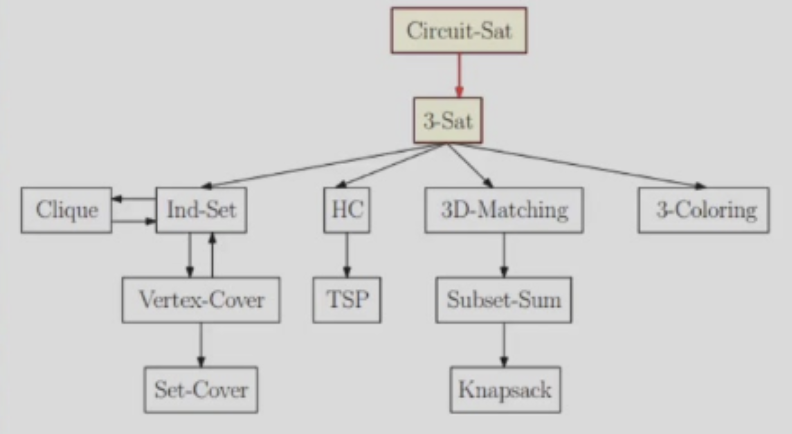
\includegraphics[width=\textwidth]{NP.png}
    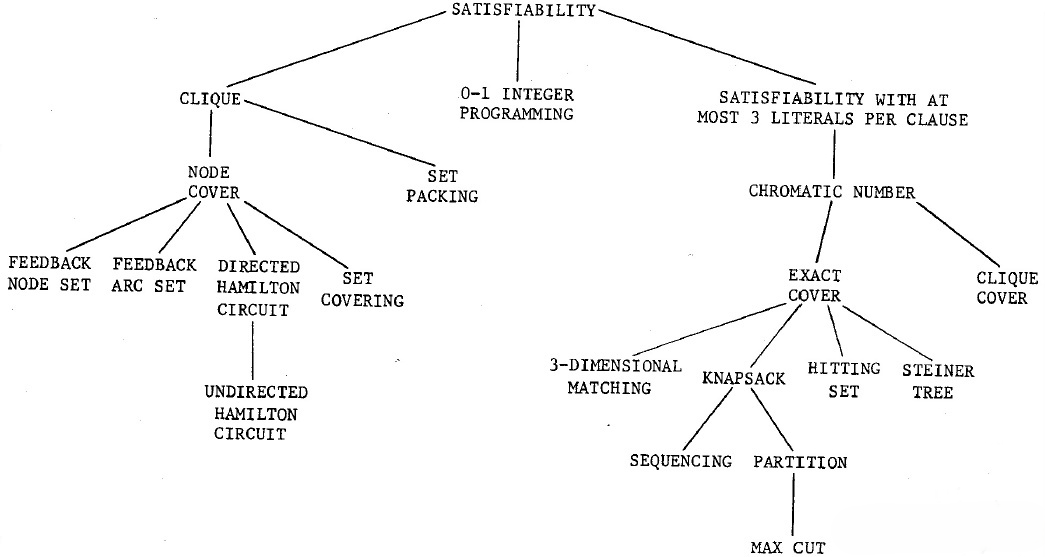
\includegraphics[width=\textwidth]{NP2.png}
\end{figure}

\begin{figure}[htbp]
    \centering
    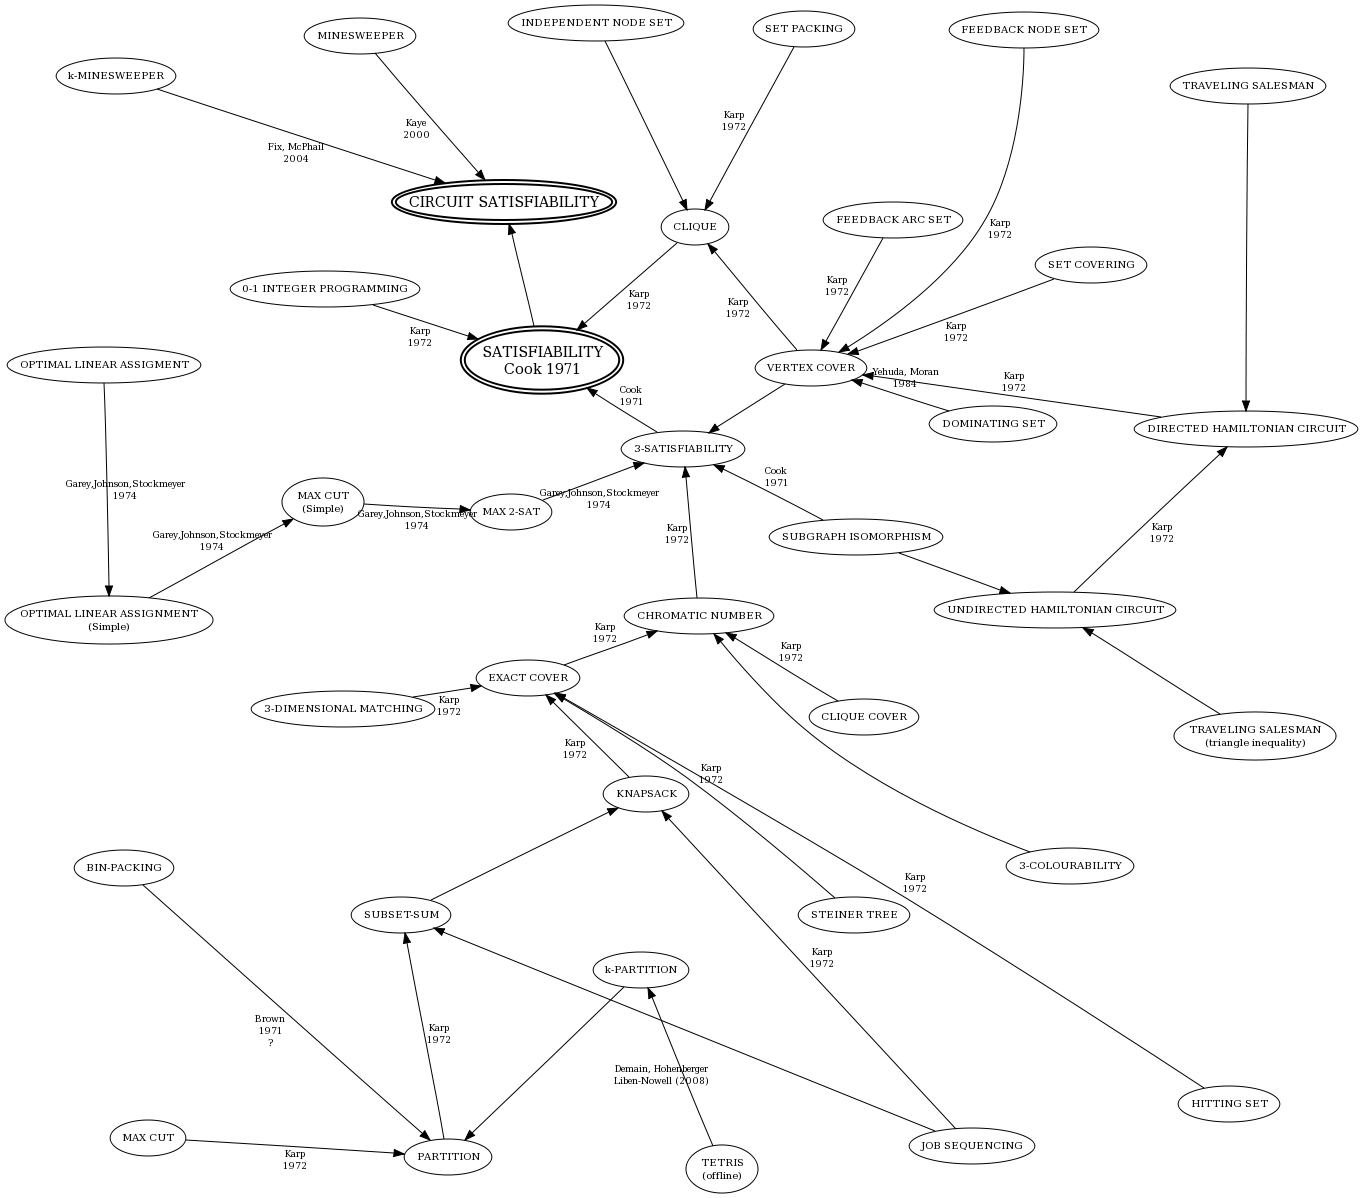
\includegraphics[width=\textwidth]{NP3.png}
\end{figure}

\newpage

\subsubsection{Self-reduction}
A problem is said to be self-reducible if the search problem reduces (by Cook reduction) in polynomial time to the decision problem.\par
\textbf{输入:}\par  
一个布尔公式 $\psi$,包含 $n$ 个变量 $x_1, x_2, \dots, x_n$。\par

\textbf{目标:}  \par
通过调用判定算法来找到一个具体的满足解(如果存在)。\par

\textbf{过程:}  \par

\textbf{1. 判定初始公式:}\par
\begin{itemize}
    \item 首先调用判定算法检查公式 $\psi$ 是否可满足:
    \begin{itemize}
        \item 如果不可满足,则直接返回“无解”;
        \item 如果可满足,则继续下一步,构造满足赋值。
    \end{itemize}
\end{itemize}\par

\textbf{2. 固定第一个变量的值:}\par
\begin{itemize}
    \item 假设公式的第一个变量是 $x_1$,尝试赋值 $x_1 = 0$,得到新的公式 $\psi_1$:
    \[
    \psi_1 = \psi \text{ 在 } x_1 = 0 \text{ 时的化简版本}。
    \]
    \item 用判定算法检查 $\psi_1$ 是否可满足:
    \begin{itemize}
        \item 如果 $\psi_1$ 可满足,说明在某个满足解中 $x_1 = 0$。将 $x_1 = 0$ 固定,递归求解剩余的变量;
        \item 如果 $\psi_1$ 不可满足,尝试 $x_1 = 1$,得到新的公式 $\psi_2$:
        \[
        \psi_2 = \psi \text{ 在 } x_1 = 1 \text{ 时的化简版本}。
        \]
        用判定算法检查 $\psi_2$ 是否可满足:
        \begin{itemize}
            \item 如果 $\psi_2$ 可满足,说明在某个满足解中 $x_1 = 1$。将 $x_1 = 1$ 固定,递归求解剩余的变量;
            \item 如果 $\psi_2$ 不可满足,说明公式 $\psi$ 不可满足。
        \end{itemize}
    \end{itemize}
\end{itemize}\par

\textbf{3. 递归处理剩余变量:}
\begin{itemize}
    \item 固定 $x_1$ 后,递归处理剩余的公式,依次固定 $x_2, x_3, \dots, x_n$,每次调用判定算法来决定当前变量的取值。
\end{itemize}\par

\textbf{4. 终止条件:}
\begin{itemize}
    \item 当所有变量 $x_1, x_2, \dots, x_n$ 都被赋值后,公式依然可满足,说明找到了一组满足解。
\end{itemize}

\begin{Theorem}
    Every NP-Complete problem/language L is self-reducible.

    每一个 NP 完全问题/语言 L 是自归约的
\end{Theorem}

指的是如果给定一个能够解决单个实例的算法或解,则可以构建一个算法来有效地解决该问题的所有其他实例。换句话说,如果你能有效解决一个小的子问题(例如,确定一个特定的元素是否应该包含在解中),你可以通过一系列这样的小问题来构建整个解。

\begin{Exercise}
    \begin{enumerate}
        \item The input of a problem will be encoded as a binary string, and the input size of a problem is the length of the encoded string.
        \item A \textcolor{red}{tautology} is a bollean formula that always evaluates to 1. 
        
        \textcolor{purple}{Tautology Problem}\par
        \textbf{Input:} A boolean formula\par
        \textbf{Output:} Whether the input formula a tautology?\par
        Then we can claim that Tautology $\in Co-NP$.
        \item To prove a reduction $A \leq_p B$, we require 3 steps:
        \item If $L_1 \le_p L_2$ and $L_2 \le_p L_3$, then $L_1 \le_p L_3$.
        \item To prove a problem $Y$ is $NP-Complete$, we need to show that $Y$ is in $NP$ , and also
    \end{enumerate}
\end{Exercise}

\textbf{Ansewer}:
\begin{enumerate}
    \item True
    \item True
    
    我在这里绕过一会儿。不过本人绕主要是和 SAT 问题搞混。 SAT 问题是是否存在使之为真的变量赋值,而 Tautology 问题则是判断一个公式是否对所有变量赋值都为真。
    
    首先要清楚,一个问题属于 NP,要求其解可以在多项式时间内验证。

    那么对于 Tautology 问题,如果验证的是非重言式,也即存在某种变量赋值使得公式为假,我们可以直接提供这个 反例 赋值,并在多项式时间内验证它。然而,虽然找到这个解的时间可能不是多项式时间,但是考虑是否是 NP 问题,我们只需要考虑验证解的时间。

    如果公式是重言式,我们需要验证它对所有可能的变量赋值都为真。这个验证过程需要检查所有 $2^n$ 种变量赋值(对于 n 个变量)。对于任意给定的解,我们无法在多项式时间内验证其正确性。
    \item 
    \begin{enumerate}
        \item We have to find the mapping function $f$ and show that it runs in polynomial time.
        
        这是归约的基础。映射函数 $f$ 的作用是将问题 $A$ 中的实例 $x$ 转换为问题 $B$ 的实例 $f(x)$。要求 $f$必须在多项式时间内运行,以保证归约不会引入额外的计算复杂性。
        \item for all $x \in A$, then $f(x) \in B$.
        
        这一条保证了归约的正确性,即问题 $A$ 的实例可以被正确地映射到问题 $B$ 的实例。如果这个条件不成立,归约可能会把问题 $A$ 的有效实例错误地映射到 $B$ 的无效实例,破坏了归约的逻辑性。
        \item If $f(x) \in B$, then $x \in A$.
        
        这一条保证了归约的完备性,即问题 $B$ 的实例确实对应问题 $A$ 的实例。如果这个条件不成立,可能会出现 $B$ 中的某些实例无法映射回 $A$ ,从而无法正确推导出 $A$ 的答案。
    \end{enumerate}

    \textbf{接下来我们讨论一下 NP 和 co-NP 的关系}

    已知的关系是 NP 和 co-NP 的交集不为空。例如 素性测试(Primality Testing)。

    \begin{itemize}
        \item [NP 中] 如果一个数是素数,可以通过提供质因数分解来快速验证。
        \item [co-NP 中] 如果一个数不是素数,可以通过提供质因数来快速验证。
    \end{itemize}

    如果 P = NP ,那么这会自动导致 P = NP = co-NP。但是如果是 NP = co-NP 却无法推出 P = NP。
    \item True
    \item Choose an NP-complete problem $X$, and show that $X \leq_p Y$.
\end{enumerate}

\newpage

\section{Approximation}
What for?——Dealing with HARD problems\par
\hspace*{\fill}\par
Getting around NP-Completeness
\begin{itemize}
    \item If N is small, even $O(2^n)$ is acceptable.
    \item Solve some important special cases in polynomial time.
    \item Find near-optimal solutions in polynomial time.
\end{itemize}\par

\hspace*{\fill}\par

Three aspects to be considered:
\begin{itemize}
    \item [A:] Optimality / Correctness (quality of a solution): For every input, the algorithm correctly solves the problem.
    \item [B:] Efficiency(cost of computations): For every input, the algorithm correctly solves the problem.
    \item [C:] General-purpose: the algorithm works for all instances.
\end{itemize}\par

\hspace*{\fill}\par

Researchers are working on
\begin{itemize}
    \item [A+C:] Exact algorithms for all instances
    \item [A+B:] Exact and fast algorithms for special cases
    \item [B+C:] Approximation algorithms 
\end{itemize}\par
Even if P=NP, still we cannot guarantee A+B+C .

\subsection{Approximation Ratio}
\begin{Definition}
    An algorithm has an \textcolor{blue}{approximation ratio} of  $\rho(n)$ if $\forall$input of size $n$, the cost $C$ of the solution produced by the algorithm is within a factor of $\rho(n)$ of the cost $C^*$ of an optimal solution:
    \begin{align*}
        \max\left( \frac{C}{C^*}, \frac{C^*}{C} \right)\le \rho(n)
    \end{align*}

    If an algorithm achieves an approximation ratio of $\rho(n)$, we call it a \textcolor{blue}{$\rho(n)$-approximation algorithm}.
\end{Definition}

\par\hspace*{\fill}\par

\begin{Definition}
    An \textcolor{blue}{approximation scheme} for an optimization problem is an approximation algorithm that takes as input not only an instance of the problem, but also a value $\textcolor{red}{\varepsilon} > 0$ such that $\forall$fixed $\varepsilon$, the scheme is a \textcolor{red}{$(1+ \varepsilon)$-approximation algorithm}.
    
    We say that an approximation scheme is a \textcolor{blue}{polynomial-time approximation scheme (PTAS)} if $\forall$ fixed $\varepsilon > 0$, the scheme runs in time polynomial in the size n of its input instance.
\end{Definition}

e.g. 
\begin{itemize}\small
    \item PTAS : $O(n^{\frac{2}{n}})$
    \item Fully polynomial-time approximation scheme (FPTAS): $O((\frac{1}{\varepsilon})^2n^3)$(关于$(\frac{1}{\varepsilon})$和$n$都是多项式级的)
\end{itemize}

我们设 $|I|$ 代表问题 I 的规模,f 是一个可计算(computable)函数,不一定为多项式函数,那么有

\begin{enumerate}
    \item PTAS(多项式时间近似方案,Polynomial time approximation scheme):存在算法 A,使得对每一个固定的 $\varepsilon \ge 0$,对任意的实例 I 都有
    $$A(I) \le (1+\varepsilon) \cdot OPT(I)$$
    且算法 A 的运行时间以问题规模 $|I|$ 的多项式为上界,则称 A 是该问题类的一个 PTAS。一般可以将 PTAS 的复杂度记为 $O(n^{f(\frac{1}{\varepsilon})})$ 。
    \item EPTAS(Efficient PTAS):在 PTAS 的基础上,要求算法 A 的复杂度是 $O(|I|^c)$ 的,其中 $c \ge 0$ 是与 $\varepsilon$ 无关的常数。可以将 EPTAS 的复杂度记为 $|I|^{O(1)}f(\frac{1}{ε})$ 。
    \item FPTAS(Fully PTAS):在 PTAS 的基础上,要求算法 A 的运行时间关于 $|I|$ 和 $\varepsilon$ 都呈多项式,即可以将 FPTAS 的复杂度记为 $|I|^{O(1)}f(\frac{1}{ε})^{O(1)}$ 。
\end{enumerate}

\subsection{Approximate Bin Packing}
Given $N$ items of sizes  $S_1 , S_2 , \dots, S_N$ , such that $0 < S_i \le 1$ , $\forall$  $1 \le i \le N$.  Pack these items in the fewest number of bins, each of which has unit capacity.

\subsubsection{Next Fit}
Place each item in a single bin until an item does not fit in. When an item doesn't fit, close it and opens a new one.\par
非常好理解但看上去有点浪费的做法,但是 Next Fit 的做法 的 approximation ratio $\le 2$。
\begin{lstlisting}
void NextFit ( ){
    read item1;
    while ( read item2 ) {
        if ( item2 can be packed in the same bin as item1 )
    place item2 in the bin;
        else
    create a new bin for item2;
        item1 = item2;
    } /* end-while */
}
\end{lstlisting}

\begin{Theorem}
    Let $M$ be the optimal number of bins required to pack a list $I$ of items.  Then next fit never uses more than $2M - 1$ bins.  There exist sequences such that next fit uses $2M - 1$ bins.
\end{Theorem}

\textbf{Proof}:\par
$ OPT(I) \ge \lceil \sum\limits_{i=1}^N S_i \rceil$. The term $\lceil \sum\limits_{i=1}^{N} S_i \rceil$ is a lower bound number of bins required to pack a list $I$ of items, and $NF(I)$ to be the number of bis used by Next Fit algorithm, respectively.\par
Let $S(B_i)$ be the size of $i-th$ bin. Let $S_j$ be the first item assigned in the $(i+1)-th$ bin, then we have $S(B_i)+S_j > 1$ , which implies that $S(B_i)+S(B_{i+1}) > 1$. \par
Then $\sum\limits_{i=1}^{N} S_i = \sum\limits_{i=1}^{NF(I)}S(B_i)$ . We can show that is Next Fit generates $2M$ (or $2M+1$ ) bins, then the optimal solution must generate at least $M+1$ bins. \par
Then $\sum\limits_{i=1}^{N} S_i > \frac{NF(I)}{2} \ge M+\frac{1}{2}$ . We obtain that $OPT(I) \ge M+1$ , since $OPT(I)$ is an integer.\par
The approximation ratio $\alpha$ of NF is
$$\alpha = \mathop{sup}\limits_I \frac{NF(I)}{OPT(I)} \le \frac{2M+1}{M+1} \le 2$$\par
We claim that the approximation ratio 2 is \textbf{tight} by showing that there exists a sequence such that the next fit uses $2M-1$ bins while the optimal solution uses $M$ bins. The instance is given below. Let $\epsilon > 0$ be a sufficiently small number. Then $I = \{ a_1,b_1,\dots,a_{2(M-1)},b_{2(M-1)},a_{2M-1},b_{2M-1}\}$ that consists of $2M-1$ large items with size $\frac{1}{2}$ and $2M-1$ small items with size $\epsilon$ and $\sum\limits_{i=1}^{2M-1} \epsilon < \frac{1}{2}$. The sequence of $I$ is one large item followed by a small item.\par
One can easily check that $NF(I)=2M-1$, in which every bin accommodates one large item and one small item. In the optimal solution, $2(M-1)$ large item occupy $M-1$ bins, while the last item is assigned together with all small items, and $OPT(I) = M$ follows.\par
This instance shows that the analysis of the approximation ratio of Next Fit is tight,i.e., $\alpha \ge \frac{2M-1}{M}$ .

\subsubsection{First FIt}
Try to place an item in the first bin that accommodates it. If no such bin is found, open a new one.\par
根据我的理解是,如果当前物品可以放入第一个箱子,则放入第一个箱子,否则按照序号再判断是否能放入下一个序号的箱子。
\begin{lstlisting}
void FirstFit ( ){
    while ( read item ) {
        scan for the first bin that is large enough for item;
        if ( found )
    place item in that bin;
        else
    create a new bin for item;
    } /* end-while */
}
\end{lstlisting}

\begin{Theorem}
    Let $M$ be the optimal number of bins required to pack a list I of items.  Then first fit never uses more than $\frac{17M}{10}$ bins. There exist sequences such that first fit uses $\frac{17(M-1)}{10}$ bins.
\end{Theorem}

\subsubsection{Best Fit}
Try to place an item in the fullest bin that can accommodate it. If there is no such bin, open a new one. Which means that place a new item in the tightest spot among all bins.\par

$T = O( N log N )$ and bin no.$\le  1.7M$

\subsubsection{On-line Algorithms}
Place an item before processing the next one, and can't change decision.\par
You never know when the input might end.  No on-line algorithm can always give an optimal solution.

\begin{Theorem}
    There are inputs that force any on-line bin-packing algorithm to use at least \textcolor{blue}{$\frac{5}{3}$} the optimal number of bins.
\end{Theorem}

\subsubsection{Off-line Algorithms}
View the entire item list before producing an answer.\par

\textcolor{red}{Trouble-maker}: The large items.\par
\textcolor{blue}{Solution}: Sort the items into non-increasing sequence of sizes.  Then apply first (or best) fit – \textcolor{blue}{first} (or \textcolor{blue}{best}) \textcolor{blue}{fit decreasing} (same as First Fit after sorting the items by decreasing order) .

\begin{Theorem}
    Let $M$ be the optimal number of bins required to pack a list $I$ of items.  Then first fit decreasing never uses more than \textcolor{blue}{$\frac{11M}{9}$} $+$ \textcolor{red}{$\frac{6}{9}$} bins.  There exist sequences such that first fit decreasing uses \textcolor{blue}{$\frac{11M}{9}$} $+$ \textcolor{red}{$\frac{6}{9}$} bins.
\end{Theorem}

\subsubsection{Inapproximability}
What is the smallest approximation ratio for the bin packing problem? In the following, we show that one cannot find an approximation algorithm with an approximation ratio smaller than 1.5 if $P \neq NP$ .\par

\begin{Theorem}
    For any constant $\epsilon > 0$, there is no $(1.5 - \epsilon)$-approximation algorithm for the bin packing problem unless P = NP.
\end{Theorem}

\textbf{Proof}:\par
Let $A = \{a_1, a_2, \dots , a_n\}$ be an instance of a PARTITION problem. We denote a set of items $B = \{\frac{2a_i}{\sum\limits_{i=1}^n a_i} | a_i \in A\}$. The bin size is 1.\par
Then items in B can be packed in 2 bins iff the set A can be partitioned into two sets with equal sums. Now suppose there is a $\rho = (1.5 - \epsilon )$ algorithm ALG for the bin packing for given $\epsilon > 0$ .\par
We use this algorithm ALG to decide if B can be packed into 2 bins. If the output of ALG is 2, clearly, we found an equal partition for A.\par
Note that $ALG \le \rho OPT$ , where OPT is the optimal value to pack the set B. If $ALG > 2$ , then it must hold that $OPT > 2$ . Otherwise, $ALG \le (1.5 - \epsilon )OPT < 3$ , which implies that $ALG = 2$ . In this case, we cannot find an equal partition.\par
In all, the approximation algorithm ALG runs in polynomial time, but it can decide whether a partition exists or not. That is, we solve the PARTITION problem, which is NP-complete, in polynomial time.\par
Therefore, we cannot have a $(1.5 - \epsilon )$-approximation algorithm for bin packing unless P = NP.

\subsection{The Knapsack Problem}
\subsubsection{fractional version}
A knapsack with a capacity  $M$  is to be packed.  Given $N$ items.  Each item  $i$  has a weight  $w_i$  and a profit  $p_i$ .  If  $x_i$ is the percentage of the item $i$  being packed,  then the packed profit will be  $p_i x_i$ .\par
We can design a greedy algorithm GreedyDensity that is based on profit density to solve the knapsack
problem.It turns out that the algorithm GreedyDensity performs badly. For example we have a bag with a capacity of $C$, and we have two kinds of items, one has a weight 1 and a profit 1, and the other has a weight $C-2$ and a profit $C-1$. The greedy algorithm will choose one item 2, however the optimal solution is to choose $C$ items 1.\par
An optimal packing is a feasible one with maximum profit (maximum profit density $\frac{p_i}{w_i}$).  That is,  we are supposed to find the values of $x_i$  such that $\displaystyle \sum_{i=1}^np_i x_i$ obtains its maximum under the constrains
\begin{align*}
    \sum_{i=1}^n w_i x_i \le M ,\ x_i\in[0,1] ,\ for\ 1\le i\le n. 
\end{align*}

\subsubsection{0-1 version}
$x_i$ is either 1 or 0. 

The approximation ratio is 2 if we are greedy on taking the maximum profit or profit density. \par
\textbf{Proof}:
\par\hspace*{\fill}\par
$$OPT = X(\text{被切掉的}) + Y(greedy)$$
$$ALG \ge max\{X,Y\}$$
$$\rho \le \frac{OPT}{ALG} \le 2$$

\subsubsection{Dynamic Programming Solution}
$W_{i, p}$ is the minimum weight of a collection from $\{1, \dots, i \}$ with total profit being  exactly $p$. 
\begin{align*}
    W_{i,p}=\left\{ \begin{array}{ll}
        \infty & i=0\\
        W_{i-1, p} & p_i>p\\
        \min\{ W_{i-1, p}, w_i+W_{i-1, p-p_i} \} & \text{otherwise}
    \end{array} \right.
\end{align*}\par
$i=1,\dots,n$, $p=1,\dots,np_{max}$. $O(n^2 p_{max})$

If $p_{max}$ is large, can round all profit values up to lie in smaller range. 
\begin{align*}
    \forall \text{ feasible solution }P,\ (1+\varepsilon)P_{alg}\le P , \ \varepsilon \ is \ precision \ parameter. 
\end{align*}

\subsection{The K-center Problem}

\begin{itemize}
    \item Input: Set of $n$ sites $s_1, \dots, s_n$
    \item Center selection problem: Select $K$ centers $C$ so that the maximum distance from a site to the nearest center is minimized.\par
    我们的目标是挑出 $K$ 个中心点,使得各个站点到最近中心的最大距离最小。
\end{itemize}

\subsubsection{Distance}
\begin{enumerate}
    \item  $dist(x, x) = 0$ (identity)
    \item $dist(x, y) = dist(y, x)$ (symmetry)
    \item $dist(x, y) \le dist(x, z) + dist(z, y)$ (triangle inequality)
\end{enumerate}
\begin{align*}
    dist(s_i , C) &= \min_{c\in C} dist(s_i, c)  \\
    &= \text{distance from $s_i$ to the closest center}\\
    r(C) &= \max_i dist(s_i, C) \\
    &= \text{smallest covering radius}
\end{align*}

\textbf{Target}: Find a set of centers $C$ that minimizes $r(C)$, subject to $|C| = K$.


\subsubsection{A Greedy Solution}
If we know that $r(C^*) \le r$ where $C^*$ is the optimal solution set, and choose center at  the site, we can verify whether $r$ meets the requirements. 

\begin{lstlisting}[language={c}]
Centers Greedy-2r(Sites S[ ], int n, int K, double r){
    Sites  S_[ ]=S[ ]; /* S_ is the set of the remaining sites */
    Centers C[ ]={ };
    while(S_ != empty){
        Select any s from S_ and add it to C;
        Delete all s_ from S_ that are at dist(s_, s) <= 2r;
    } /* end-while */
    if (|C|<=K) return C;
    else ERROR(No set of K centers with covering radius at most r);
}
\end{lstlisting}
\begin{Theorem}
    Suppose the algorithm selects more than $K$ centers.  Then for any set $C^*$ of size at most $K$, the covering radius is $r(C^*) > r$.
\end{Theorem}

任意两点间距离一定小于直径,那么若知道最优解 $r(C^*)$ 则取两倍最优解半径,去掉 $2r(C^*)$ 内的点。再任意选取一个未被去掉的点。迭代 $k$ 次即为答案。

Binary search for $r$ to know $r(C^*)$. Solution radius is $2r_1$ --- 2-approximation. 

Or
\begin{lstlisting}[language={c}]
Centers Greedy-Kcenter(Sites S[ ], int n, int K){
    Centers  C[ ] = { };
    Select any s from S and add it to C;
    while (|C|<K) {
        Select s from S with maximum dist(s, C);
        Add s it to C;
    } /* end-while */
    return C;
}
\end{lstlisting}
\begin{Theorem}
    The algorithm returns a set $C$ of $K$ centers such that $r(C) \le 2r(C^*)$ where $C^*$ is an optimal set of $K$ centers.(2-approximation)
\end{Theorem}\par

Greedy-2r 算法在给定最优解 $r(C^*)$ 的情况下是一个 2-近似算法。

如果 Greedy-2r 算法在 K 步之内不停止,那么最优解一定不是 $r(C^*)$(即会大于 $r(C^*)$ )。

可以由二分查找的思路不断判断 $r(C^*)$ 选择是否合适。

\begin{Theorem}
    Unless P = NP, there is no  $\rho$-approximation for center-selection problem for any $\rho < 2$.
\end{Theorem}

\textbf{Attention}: $\rho < 2$ and it cannot be equal.

\begin{Exercise}
    \begin{enumerate}
        \item For every instance $I$, let $C(I)$ be the cost of the approximation algorithm on the input $I$ and $OPT(I)$ be the optimal cost on the input $I$ ,respectively. The approximation ration $\alpha$ for a minimization problem, is defined to be
        \item Which of the following running time statement is not correct?
        \begin{enumerate}
            \item [A] $O(n^{\frac{1}{\epsilon}})$ is a PTAS
            \item [B] $O(n^{3} 2^{\frac{1}{\epsilon}})$ is a FPTAS
            \item [C] $O(n^{\frac{4}{\epsilon^2}+1})$ is a PTAS
            \item [D] $O(nlog(\frac{1}{\epsilon})+\frac{1}{\epsilon^4})$ is a FPTAS
        \end{enumerate}
        \item We use a balanced binary search tree to implement the First Fit algorithm, which take $O(n logn)$ time. Choose the correct ordering of the tree.
        \begin{enumerate}
            \item [A] The ordering of the tree is by the remaining capacity of bin.
            \item [B] The ordering of the tree is by the bin index.
        \end{enumerate}
        \item For any constant $\epsilon > 0$ , there is no $(1.5 - \epsilon)$-approximation algorithm for the bin packing problem unless $P = NP$ .
        \item In the knapsack problem, we sort all the items by the ratio of their profits to their sizes so that $\frac{p_1}{w_1} \ge \frac{p_2}{w_2} \ge \dots \ge \frac{p_n}{w_n}$\par
        The greedy algorithm GreedyDensity will select items in this order until exceed the capacity of the knapsack. \par
        The approximation ratio of GreedyDensity is 2.
        \item The approximation ratio of the algorithm Greedy-Kcenter for arbitrary distance (may not be metric distance ) is at most 2.
    \end{enumerate}
\end{Exercise}

\textbf{Ansewer}:
\begin{enumerate}
    \item $\alpha = sup_I\frac{C(I)}{OPT(I)}$ (attention for sup, it can be easily forget) 
    \item B
    \item B, since A is for any fit. However this question can cause ambiguity.
    \item True
    \item False
    \item False. It's at least 2 and unless P = NP, could be $\rho(\rho < 2)$ .
\end{enumerate}

\newpage
\section{local search}
Solve problems approximately —— aims at a local optimum. 

Framework of Local Search:
\begin{itemize}\small
    \item [\textbf{Local}]
    \subitem Define neighborhoods in the feasible set. 
    \subitem A local optimum is a best solution in a neighborhood. 
    \item [\textbf{Search}]
    \subitem Start with a feasible solution and search a better one within the neighborhood. 
    \subitem A local optimum is achieved if no improvement is possible. 
\end{itemize}

Neighbor Relation:
\begin{itemize}\small
    \item  $S \sim S'$ : $S'$ is a neighboring solution of $S$ --- $S'$ can be obtained by a small modification of $S$.
    \item  $N(S)$: neighborhood of $S$ --- the set $\{ S': S \sim S' \}$.
\end{itemize}
\begin{lstlisting}[language={c}]
SolutionType Gradient_descent(){
    Start from a feasible solution S in FS;
    MinCost=cost(S);
    while(1){
        S_ = Search(N(S));  /* find the best S_ in N(S) */
        CurrentCost=cost(S_);
        if(CurrentCost<MinCost){
            MinCost=CurrentCost;    
            S=S_;
        }
        else break;
    }
    return S;
}
\end{lstlisting}

\subsection{The Vertex Cover Problem}
一个要求更高的版本:\par

Given an undirected graph $G = (V, E)$. Find a \textcolor{red}{minimum} subset $S$ of $V$ such that for each edge $(u, v)$ in $E$, either $u$ or $v$  is in $S$.

\begin{itemize}
    \item Feasible solution set $FS$ : all the vertex covers. 
    \item $cost(S)=|S|$
    \item $S\sim S'$: Each vertex cover $S$ has at most $|V|$ neighbors
    \item Search: Start from $S = V$; delete a node and check if $S'$ is a vertex cover with a smaller cost.
\end{itemize}

\subsection{Simulated Annealing}
The material is cooled very gradually from a high temperature, allowing it enough time to reach equilibrium at a succession of intermediate lower temperatures.

Cooling schedule:  $T = \{ T_1 , T_2 , \dots \}$

\subsubsection{The Metropolis Algorithm}

这段代码实现的是模拟退火算法(Simulated Annealing, SA)的一个变种——Metropolis 算法,它是一种用于求解优化问题的随机搜索算法。该算法旨在找到一个定义在有限或无限搜索空间上的函数的最大值或最小值。在这个例子中,目标是寻找一个成本函数的最小值。

\begin{lstlisting}[language={c}]
SolutionType Metropolis( ){
    Define constants k and T;
    Start from a feasible solution S in FS ;
    MinCost = cost(S);
    while (1) {
        S_ = Randomly chosen from N(S); 
        CurrentCost = cost(S_);
        if ( CurrentCost < MinCost ) {
            MinCost = CurrentCost;    S = S_;
        }
        else {
            With a probability exp(-d(cost(S_))/kT), let S = S_;
            else  break;
        }
    }
    return S;
}
\end{lstlisting}

$k$ 是玻尔兹曼常数,在物理应用中用来将能量转换为温度单位。这里的 $k$ 可以被视为1或者省略,因为它是比例因子,不影响选择的概率。 $T$ 是当前的温度,它控制着接受更差解的概率。随着算法的进行, $T$ 会逐渐降低。


从可行解空间 $FS$ 中选择一个初始解 $S$ 。这个初始解可以是随机选择的,或者是通过某种启发式方法得到的。

计算初始解的成本,并将其设为当前最小成本 $MinCost$。接下来是一个无限循环 $(while (1))$ ,其目的是不断探索解空间直到满足某个终止条件(例如,达到预设的迭代次数、温度降到非常低或找不到更好的解等)。

在当前解 $S$ 的邻域 $N(S)$ 中随机选择一个新的候选解 $S\_$ 。邻域是指与当前解相近的一组解,通常通过对当前解进行小幅度的修改来生成。

如果新候选解的成本比当前最低成本要低,则更新最低成本和当前解。如果新候选解的成本更高,那么根据 Metropolis 准则,仍然有一定概率接受这个更差的解。这个概率由指数函数 $exp(-d(cost(S\_))/kT)$ 给出,其中 $d(cost(S\_))$ 是新解的成本与当前最优解的成本之差。这个概率确保了算法能够在早期阶段跳出局部最优解,从而有机会探索更广阔的解空间。

根据上述概率决定是否接受新的更差的解。如果接受了,则设置 $S = S\_$ ;否则,这里使用了 break 语句,然而在标准的模拟退火或 Metropolis 算法中,应该继续搜索而不是退出循环。正确的做法可能是拒绝此更差的解并保持原状,继续下一轮迭代。最终返回找到的最佳解 $S$ 。

\subsection{Hopfield Neural Networks}
Graph $G = (V, E)$ with integer edge weights $w$ (positive or negative).
\begin{itemize}
    \item If $w_e < 0$, where $e = (u, v)$, then $u$ and $v$ want to have the same state($\pm 1$). 
    \item if $w_e > 0$ then $u$ and $v$ want different states.
\end{itemize}

The absolute value $|w_e|$ indicates the strength of this requirement.

Output: a configuration $S$ of the network —— an assignment of the state $s_u$ to each node $u$. 

There may be \textcolor{red}{no} configuration that respects the requirements imposed by \textcolor{red}{all} the edges.

Find a configuration that is sufficiently good.

\begin{Definition}
    In a configuration $S$, edge $e = (u, v)$ is good if $w_e s_u s_v < 0$ ($w_e < 0$ iff $s_u = s_v$ ); otherwise, it is bad.
\end{Definition}
\begin{Definition}
    In a configuration $S$, a node $u$ is satisfied if the weight of incident good edges $\ge$ weight of incident bad edges.
    \begin{align*}
        \sum_{v:e=(u,v)\in E}w_es_us_v\le 0
    \end{align*}
\end{Definition}
\begin{Definition}
    A configuration is stable if all nodes are satisfied. 
\end{Definition}

Does a Hopfield network always have a stable configuration, and if so, how can we find one?

A Hopfield network has an associated \textbf{energy function} \( E(\mathbf{s}) \) that can be used to assess the stability of a state. The state of the network is represented by a vector of neuron activations $\mathbf{s} = (s_1, s_2, \dots, s_N)$ , where each $s_i$ is typically $\pm 1$ . The energy function is defined as:

Hopfield 网络有一个关联的 \textbf{能量函数} $E(mathbf{s})$,可用于评估状态的稳定性。网络的状态由神经元激活向量 $E(s) = (s_1, s_2, dots, s_N)$ 表示,其中每个 $s_i$ 通常为 $\pm 1$ 。能量函数定义为:

$$E(\mathbf{s}) = -\frac{1}{2} \sum_{i=1}^N \sum_{j=1}^N w_{ij} s_i s_j$$

where $w_{ij}$ are the weights of the connections between neurons $i$ and $j$ , and typically the network is designed such that the weight matrix is symmetric, i.e., $w_{ij} = w_{ji}$ and $w_{ii} = 0$ for all $i$ .

This energy function has the following key properties:
\begin{itemize}
    \item \textbf{Local Minima}: The energy function is a scalar value that decreases when the network updates its states to configurations that reduce the number of disagreements between neurons. Each local minimum corresponds to a stable configuration of the network.
    
    能量函数是一个标量值,当网络将其状态更新为减少神经元之间不一致数量的配置时,该标量值会减小。每个本地最小值对应于网络的稳定配置。
    \item \textbf{Monotonicity}: The energy function decreases with every update of the state, which means that the network will always move towards lower-energy configurations. The update rule for the network (typically asynchronous updates) guarantees that the energy will never increase.
    
    能量函数会随着状态的每次更新而减少,这意味着网络将始终朝着更低功耗的配置发展。网络的更新规则(通常是异步更新)保证能量永远不会增加。
\end{itemize}

A Hopfield network's state will stabilize in one of the local minima of the energy function. This means that once the network reaches a stable state, no further changes will occur because the energy will be at a local minimum, where each neuron is in a configuration that minimizes its individual energy contribution.

\subsubsection{State-flipping Algorithm}
\begin{lstlisting}[language={c}]
ConfigType State_flipping(){
    Start from an arbitrary configuration S;
    while(!IsStable(S)){
        u = GetUnsatisfied(S);
        su = -su;
    }
    return S;
}
\end{lstlisting}
\textbf{Claim}\par
The state-flipping algorithm terminates at a stable configuration after at most $\displaystyle W = \sum_e|w_e|$ iterations.\par

This is because the energy function decreases monotonically with each update, and the total number of updates is bounded by the sum of the absolute values of the weights in the network.

能量函数随每次更新单调递减,而更新的总次数以网络中权重的绝对值之和为界(最多就是一次减一直至减为0)。不过,我个人认为还有一个界是一共 $n$ 个点,那最多其实就是 $2^n$ 种可能,也即另一个上界。

Related to Local Search:
\begin{itemize}
    \item [Problem:]  To maximize $\Phi$.
    \item [Feasible solution] set FS: configurations
    \item [$S\sim S'$:] $S'$ can be obtained from $S$ by flipping a single state
\end{itemize}
\textbf{Claim}\par
Any local maximum in the state-flipping algorithm to maximize $\Phi$ is a stable configuration.\par

\textbf{Is it a polynomial time algorithm?}\par
Still an open question: to find an algorithm that constructs stable states in time polynomial in $n$ and $\log W$ (rather than $n$ and $W$ ), or in a number of primitive arithmetic operations that is polynomial in n alone, independent of the value of $W$ .

\subsection{The Maximum Cut Problem}
Given an undirected graph $G = (V, E)$ with positive integer edge weights $w_e$, find a node partition $(A, B)$ such that the total weight of edges crossing the cut is maximized.
\begin{align*}
    w(A,B):=\sum_{u\in A, v\in B}w_{uv}
\end{align*}

Related to Local Search:
\begin{itemize}
    \item [Problem:]  To maximize $\displaystyle \Phi(S)=\sum_{e\text{ is good}}|w_e|$.
    \item [Feasible solution] set FS: any partition $(A, B)$ 
    \item [$S\sim S'$:] $S'$ can be obtained from $S$ by moving one node from $A$ to $B$, or one from $B$ to $A$.
\end{itemize}

\begin{itemize}
    \item [Toy] application:
    \subitem n activities, m people.
    \subitem Each person wants to participate in two of the activities.
    \subitem Schedule each activity in the morning or afternoon to maximize number of people that can enjoy both activities.
    \item [Real] applications:
    \subitem Circuit layout, statistical physics
\end{itemize}\par

A special case of Hopfield Neural Network with $w_e$ all being positive. 

\textbf{Claim}\par

Let $(A, B)$ be a local optimal partition and let $(A^*, B^*)$ be a global optimal partition.  Then $w(A, B) \ge \frac{1}{2} w(A^*, B^*) = \frac{1}{2}OPT$ . The approximation ratio of 2 follows from $\frac{OPT}{w(A, B)} \le 2$.\par

\textbf{Proof}\par

Since $(A,B)$ is a local optimal partition, for any $u \in A$
$$\sum\limits_{v \in A}w_{uv} \le \sum\limits_{v \in B}w_{uv}$$

Summing up foe all $u \in A$

$$2\sum\limits_{\{u,v\} \subset A}w_{uv} = \sum\limits_{u \in A}\sum\limits_{v \in A}w_{uv} \le \sum\limits_{u \in A}\sum\limits_{v \in B}w_{uv} = w(A,B)$$

$$2\sum\limits_{\{u,v\} \subset B}w_{uv} \le w(A,B)$$

$$w(A*,B*) \le \sum\limits_{\{u,v\} \subset A}w_{uv} + \sum\limits_{\{u,v\} \subset B}w_{uv} + w(A,B) \le 2w(A,B)$$

\begin{itemize}
    \item [1976] Sahni-Gonzales  There exists a 2-approximation algorithm for MAX-CUT.
    \item [1995] Goemans-Williamson  There exists a 1.1382( $\mathop{min}\limits_{0 \le \theta \le \pi} \frac{\pi}{2}\frac{1-\cos \theta}{\theta}$ )-approximation algorithm for MAX-CUT.
    \item [1997] Håstad Unless P = NP, no $\frac{17}{16}$(1.0625) approximation algorithm for MAX-CUT.
\end{itemize}

而我们目前还没有找到一个多项式时间的算法来解决这一问题。

\subsubsection{Big-improvement-flip}

However, it may NOT in polynomial time. So we choose to stop the algorithm when there are no “big enough” improvements.

Only choose a node which, when flipped, increases the cut value by at least
\begin{align*}
    \frac{2\varepsilon}{|V|}w(A,B)
\end{align*}

\textbf{Claim}\par
Upon termination, similarly, we could get that the big-improvement-flip algorithm returns a cut $(A, B)$ so that
\begin{align*}
    (2+\varepsilon)w(A, B)\ge w(A^*, B^*)
\end{align*}

Since $\forall x\ge 1$, we have $\left( 1+\frac{1}{x} \right)^x\ge 2$, so the objective function doubles at least every $\frac{n}{\varepsilon}$  flips.

\textbf{Claim}\par
The big-improvement-flip algorithm terminates after at most $O\left( \frac{n}{\varepsilon}\log W \right)$ flips.

\subsubsection{K-L heuristic}

The neighborhood of a solution should be \textcolor{blue}{rich enough} that we do not tend to get stuck in bad local optima; but the neighborhood of a solution should \textcolor{blue}{not be too large}, since we want to be able to efficiently search the set of neighbors for possible local moves.

$$Single-flip \Rightarrow k-flip \Rightarrow \Theta (n^k)\  for \ searching \ in \ neighbors$$

A better local, k-flip. 
\begin{enumerate}
    \item [Step 1] make 1-flip as good as we can - $O(n)$ $\Rightarrow$ $(A_1, B_1)$ and $v_1$
    \item [Step k] make 1-flip of an unmarked node as good as we can - $O(n-k+1)$ $\Rightarrow$ $(A_k, B_k)$ and $v_1, \dots, v_k$
    \item [Step n] $(A_n, B_n)=(B, A)$
\end{enumerate}

我个人的理解是到了第 $k$ 步时,已经与原来的 $(A,B)$ 有 $k$ 个节点不同了,也即邻域达到了 $\Theta (n^k)$。

这个第 $n$ 步,它的作用可能在于确保最后得到的解具有某种对称性、平衡性或对偶性。通过这种交换,算法能够调整结构,确保最终的稳定状态符合优化问题的要求。

Neighborhood of $(A, B) = \{ (A_1, B_1), \dots, (A_{n-1}, B_{n-1}) \}$ - $O(n^2)$

\newpage

\section{Randomized Algorithms}

我们学过的快排(quicksort)的时间复杂度是多少?期望下是 $O(n \log n)$,最坏情况下是 $O(n^2)$。而快排是确定性算法,即它的行为是确定的,不会因为输入的不同而改变。

\begin{enumerate}\small
    \item What to Randomize?
    \subitem Average-case Analysis: The world behaves randomly —— randomly generated input solved by traditional algorithm
    \subitem Randomized Algorithms: The algorithm behaves randomly —— make random decisions as the algorithm processes the worst-case input
    \item Why Randomize?
    \subitem Efficient deterministic algorithms that always yield the correct answer are a special case of 
    \begin{itemize}
        \item [蒙特卡罗算法] efficient randomized algorithms that only need to yield the correct answer with \textcolor{blue}{high probability}. 
        \item [拉斯维加斯算法] randomized algorithms that are always correct, and run efficiently \textcolor{blue}{in expectation}. 
    \end{itemize}
\end{enumerate}

\subsection{A Quick Review}
\begin{itemize}
    \item $Pr[A]:=$ the \textcolor{blue}{probability} of the event $A$
    \item $\bar{A}:=$ the \textcolor{blue}{complementary} of the event $A$ ($A$ did not occur )
    \begin{align*}
        Pr[A]+Pr[\bar{A}]=1
    \end{align*}
    \item $E[X]:=$ the \textcolor{blue}{expectation} (the ``average value'') of the random variable X
    \begin{align*}
        E[X]=\sum_{j=0}^\infty j \cdot Pr[X=j]
    \end{align*}
\end{itemize}

\subsection{The Hiring Problem}
\begin{itemize}
    \item Hire an office assistant from headhunter 
    \item Interview a different applicant per day for $N$ days
    \item Interviewing Cost = $C_i$  $\ll$  Hiring Cost = $C_h$
    \item Analyze interview \& hiring cost instead of running time
\end{itemize}
Assume M people are hired.  

Total Cost: $O(NC_i + MC_h)$

\subsubsection{Naïve Solution}
\begin{lstlisting}[language={c}]
int Hiring(EventType C[], int N){ /* candidate 0 is a least-qualified dummy candidate */  
    int Best = 0;
    int BestQ = the quality of candidate 0;
    for(i=1;i<=N;i++){
        Qi = interview(i); /* Ci */
        if(Qi>BestQ){
            BestQ = Qi;
            Best = i;
            hire(i);  /* Ch */
        }
    }
    return Best;
}
\end{lstlisting}
Worst case: The candidates come in increasing quality order $O(NC_h)$

\subsubsection{Assume candidates arrive in random order}
Randomness assumption: any of first $i$ candidates is equally likely to be best-qualified so far. 
\begin{align*}
    X &= \text{number of hires}\\
    E[X]&=\sum_{j=1}^N j\cdot Pr[X=j]\\
    X_i&=\left\{ \begin{array}[c]{ll}
        1 & \text{if candidate $i$ is hired}\\
        0 & \text{if candidate $i$ isn't hired}
    \end{array} \right.\\
    \Rightarrow&X=\sum_{i=1}^N X_i \\
    & E[X_i]=Pr[\text{candidate $i$ is hired}]=\frac{1}{i}\\
    \Rightarrow&E[X]=E\left[ \sum_{i=1}^NX_i \right]=\sum_{i=1}^N E[X_i]\\
    \Rightarrow& O(C_h \ln N + N C_i)
\end{align*}
Radomized Algorithm: takes time to randomly permute the list of candidates, but no longer need to assume that candidates are presented in random order. Also the algorithm may need to be off-line.

\begin{lstlisting}
int RandomizedHiring ( EventType C[ ], int N ){
    /* candidate 0 is a least-qualified dummy candidate */
    int Best = 0;
    int BestQ = the quality of candidate 0;

    randomly permute the list of candidates;

    for ( i=1; i<=N; i++ ) {
        Qi = interview( i ); /* Ci */
        if ( Qi > BestQ ) {
            BestQ = Qi;
            Best = i;
            hire( i );  /* Ch */
        }
    }
}
\end{lstlisting}

\paragraph{Radomized Permutation Algorithm}\quad 

\textbf{Target}: Permute array $A[]$. 

Assign each element $A[ i ]$ a random priority $P[ i ]$, and sort. 
\begin{lstlisting}[language={c},mathescape = true]
void PermuteBySorting(ElemType A[ ], int N){
    for(i=1;i<=N;i++)
        A[i].P = 1 + rand()%( `$N^3$` ); 
        /* makes it more likely that all priorities are unique */
    Sort A; /* using P as the sort keys*/
}
\end{lstlisting}

PermuteBySorting produces a uniform random permutation of the input, assuming all priorities are distinct.

\subsubsection{Online Hiring Algorithm - hire only once}

要比前面 k 个候选者中质量最高的那个更好,才能被雇佣。

\begin{lstlisting}[language={c}]
int OnlineHiring(EventType C[ ], int N, int k ){
    int Best = N;
    int BestQ = -`$\infty$` ;
    for(i=1 ; i<=k ; i++){
        Qi = interview(i);
        if(Qi>BestQ) BestQ = Qi;
    }
    for(i=k+1;i<=N;i++){
        Qi = interview(i);
        if(Qi>BestQ){
            Best = i;
            break;
        }
    }
    return Best;
}
\end{lstlisting}

$S_i:=$ the $i$-th applicant is the best. 

$S_i$ is true if
\begin{align*}
    &\{ A:= \text{the best one is at position $i$} \} \\
    \cap &\{ B:=  \text{no one at positions $k+1 \sim i-1$ are hired} \}    
\end{align*}
$A$ and $B$ are independent. 

\begin{align*}
    Pr[S_i]&=Pr[A\cap B]=Pr[A]\cdot Pr[B]\\
    &=\frac{1}{N}\frac{k}{(i-1)}=\frac{k}{N(i-1)}\\
    Pr[S]&=\sum_{i=k+1}^N Pr[S_i]=\sum_{i=k+1}^N\frac{k}{N(i-1)}=\frac{k}{N}\sum_{i=k}^{N-1}\frac{1}{i}
\end{align*}

$$\text{Since} \int_k^{k+1} \frac{1}{x} dx \le \frac{1}{k} \le \int_{k-1}^{k} \frac{1}{x} dx$$

$$\int_k^N \frac{1}{x} dx \le \sum\limits_{i=k}^{N-1}\frac{1}{i} \le \int_{k-1}^{N-1} \frac{1}{x} dx$$

The probability we hire the best qualified candidate for a given $k$:
\begin{align*}
    \frac{k}{N}\ln\left( \frac{N}{k} \right)\le Pr[S] \le \frac{k}{N}\ln\left( \frac{N-1}{k-1} \right)
\end{align*}

The best value of $k$ to maximize the above probability:
\begin{align*}
    f(k)&=\frac{k}{N}\ln\left( \frac{N}{k} \right)\\
    f'(k)&=\frac{1}{N}\ln\left( \frac{N}{k} \right)-\frac{1}{N}=0\\
    k&=\frac{N}{e}\\
    f_{max}\left(\frac{N}{e}\right)&=\frac{1}{e}
\end{align*}

\subsection{Quicksort}
Deterministic Quicksort
\begin{itemize}
    \item $\Theta (N^2)$ worst-case running time
    \item $\Theta(N \log N)$ average case running time, assuming every input permutation is equally likely    
\end{itemize}

\subsubsection{Proof for average case running time}

我们先从直觉上说明为什么:如果在递归的每一层上, randomized-partition 所做出的划分使任意固定量的元素偏向划分的某一边,则算法递归树的深度为 $\Theta(\log N)$ ,且在每一层上所做的工作量都为 $O(n)$ 。在这些层次之间,即使我们增加了新的、最具有不对称性的划分的层次,总的运行时间仍然是 $O(n \log n)$ 。

\textbf{运行时间和比较}

QUICKSORT 的运行时间是由花在过程 PARTITION 上的时间所决定的。每当 PARTITION 过程被调用时,就要选出一个主元元素。后续对 QUICKSORT 和 PARTITION 的各次递归调用中,都不会包含该元素。于是,在快速排序算法的整个执行过程中,至多只可能调用 PARTITION 过程 n 次。

为了便于分析,我们将数组 A 的各个元素重新命名为 $z_1,z_2,\dots,z_n$ ,其中 $z_i$ 是数组 A 中的第 i 个最小的元素。此外,我们还定义 $Z_{ij} = \{z_i,z_{i+1},\dots,z_j\}$ 为 $z_i$ 与 $z_j$ 之间(包含这两个元素)的元素集合。

那么,算法何时会比较 $z_i$ 与 $z_j$ 呢?我们首先观察到每一对元素至多比较一次,因为各个元素仅与主元元素进行比较,并且,在某一次 PARTITION 调用结束之后,该次调用中所用到的主元元素就再也不会与任何其他元素进行比较了。

此时我们定义 

$$X_{ij} = \begin{cases} 1 & \text{if } z_i \text{ and } z_j \text{ are compared} \\ 0 & \text{otherwise} \end{cases}$$

我们要考虑的是在算法的执行过程中,是否有任何的比较发生,而不是在循环的一次选代或对 PARTITION 的一次调用中是否有比较发生。因为每一对元素至多被比较一次,因而,我们可以很容易地刻划算法所执行的总的比较次数:

$$X = \sum\limits_{i=1}^{n-1}\sum\limits_{j=i+1}^{n}X_{ij}$$

对上述式子求期望,利用期望的性质我们可以得到:

$$E[X] = \sum\limits_{i=1}^{n-1}\sum\limits_{j=i+1}^{n}E[X_{ij}] = \sum\limits_{i=1}^{n-1}\sum\limits_{j=i+1}^{n}Pr\{z_i \ and \ z_j \ are \ compared\}$$

此时我们再来考虑两个元素何时不进行比较。一般而言,一旦一个满足 $z_i < x < z_j$ 的主元 $x$ 被选择后,我们知道 $z_i$ 与 $z_j$ 以后再也不会可能进行比较了。另一方面,如果 $z_i$ 在 $Z_{ij}$ 中的所有其他元素之前被选为主元,那么 $z_i$ 就将与 $Z_{ij}$ 中、除了它自己以外的所有其他元素进行比较。

由此我们知道, $z_i$ 会与 $z_j$ 进行比较,当且仅当 $Z_{ij}$ 中将被选作主元的第一个元素是 $z_i$ 或 $z_j$ 。

我们现在来计算这一事件的概率。在 $Z_{ij}$ 中的某一元素被选为主元之前,集合 $Z_{ij}$ 整个都是在同一划分中的。于是 $Z_{ij}$ 中的任何元素都会等可能地被首先选为主元。因为集合 $Z_{ij}$ 中共有 $j-i+1$ 个元素,所以,任何元素被首先选为主元的概率为 $\frac{1}{j-i+1}$ 。

于是我们有:

$$Pr\{z_i \ and \ z_j \ are \ compared\} = Pr\{z_i \ or z_j \text{是从} Z_{ij} \text{中第一个被选为主元的元素}\} = \frac{2}{j-i+1}$$

$$\therefore E[X] = \sum\limits_{i=1}^{n-1}\sum\limits_{j=i+1}^{n}\frac{2}{j-i+1} \mathop{=}\limits^{k = j - i} \sum\limits_{i=1}^{n-1}\sum\limits_{k=1}^{n-i}\frac{2}{k+1} < \sum\limits_{i=1}^{n-1}\sum\limits_{k=1}^{n}\frac{2}{k} = \sum\limits_{i=1}^{n-1}O(\log n) = O(n \log n)$$

\par\hspace*{\fill}\par
\par\hspace*{\fill}\par
\par\hspace*{\fill}\par

Central splitter $:=$ the pivot that divides the set so that each side contains at least $n/4$

Modified Quicksort $:=$ always select a central splitter before recursions

The expected number of iterations needed until we find a central splitter is at most 2. (As $P = \frac{1}{2}$ , E = 2)

\begin{align*}
    Pr[\text{find a central splitter}]=\frac{1}{2}
\end{align*}

Type $j$ : the subproblem $S$ is of type $j$ if
\begin{align*}
    N\left( \frac{3}{4} \right)^{j+1}\le |S|\le N\left( \frac{3}{4} \right)^j
\end{align*}

在这里我们把子问题定义为比较次数。所以这个子问题规模的大小遵循上述。

对于 type j 的子问题,由于每一个子问题加起来总共是 N 个,因此最多是有 $(\frac{4}{3})^{j+1}$ 个。

There are at most $\left( \frac{4}{3} \right)^{j+1}$ subproblems of type $j$.
\begin{align*}
    &\left.\begin{array}[c]{l}
        E[T_{type\ j}]=O\left( N\left( \frac{3}{4} \right)^j \right)\times \left( \frac{4}{3} \right)^{j+1}=O(N)\\
        \text{Number of different types }=\log_{4/3}N=O(\log N)
    \end{array}\right\}\\
    &\therefore O(N\log N)
\end{align*}

\subsection{Max 3-SAT}

In the max 3-SAT problem, we are given a 3-SAT formula and our goal is to find a truth assignment that satisfies as many clauses as possible.

Let us consider a simple randomized algorithm. Flip a coin, and set each variable true with probability $\frac{1}{2}$ , independently for each variable.

Given a 3-SAT formula with k clauses, the expected number of clauses satisfied by a random assignment is $\frac{7k}{8}$.

接下来让我们来证明它。

Let 

$$X_i = \begin{cases} 1,& \text{if } Clause_i \text{ is satisfied}\\ 0,& \text{otherwise}\end{cases}$$

Note that the probability of a clause is satisfied is $\frac{7}{8}$ . We obtain that

$$E(X) = \sum\limits_{i=1}^kE(X_i) = \sum\limits_{i=1}^k Pr(X_i=1) = \frac{7k}{8}$$

The probability that a random assignment satisfies at least $\frac{7k}{8}$ clauses is at least $\frac{1}{8k}$ .

接下来让我们来证明。

Let $p_j$ be probability that exactly j clauses are satisfied. By the expectation of X, we have

$$\frac{7}{8} = E(X) = \sum\limits_{j=1}^kjp_j$$
$$ = \sum\limits_{j=1}^{j < \frac{7}{8}k}jp_j + \sum\limits_{j < \frac{7}{8}k}^k jp_j$$
$$\le \frac{7}{8}k \sum\limits_{j=1}^{j < \frac{7}{8}k}p_j + k \sum\limits_{j< \frac{7}{8}k}^k p_j$$
$$\le (\frac{7}{8}k - \frac{1}{8}) + k Pr[X > \frac{7k}{8}]$$

The last inequality is satisfied because the number of satisfied clauses is an integer. Therefore, we have $Pr[X > \frac{7k}{8}] \ge \frac{1}{8k}$ .

\subsection{Max-cut}
A simple randomized algorithm by Erdos for the maximum cut problem. For each vertex, flip a coin: if the coin comes up heads, put the vertex in A, otherwise, put in it B .

Let (A, B) be the cut returned by the algorithm, then $E[w(A, B)] \ge \frac{OPT}{2}$ , where OPT is the optimal value of the maximum cut problem.

$$E[w(A,B)] = E[\sum\limits_{(u,v) \in E} X_{uv}] = \sum\limits_{(u,v) \in E} Pr[X_{uv} = 1]$$

On the other hand,

$$Pr[X_{uv} = 1] = \frac{1}{2}$$

Thus,

$$E[w(A,B)] \ge \frac{|E|}{2} \ge \frac{OPT}{2}$$

\subsubsection{Markov's inequality}
Let X be a real-valued random variable that assumes only nonnega-tive values. Then for all $a > 0$ , $Pr[X \ge a] \le \frac{E[X]}{a}$

\subsubsection{Reverse Markov's inequality}
Let Y be a random variable that is never larger than B. Then, for all $a < B$ , $Pr[Y \le a] \le \frac{E[B - Y]}{B - a}$

Consider a random trial in which the probability of success is p. If we perform k mutually independent trials,
then

$$P[all \ failure] = (1-p)^k \le e^{-pk}$$

and therefore,

$$P[at \ least \ one \ success] = 1 - (1-p)^k \ge 1 - e^{-pk}$$

\subsection{Exercise}
\begin{enumerate}
    \item We have m balls and m boxes. Each ball is assigned to one of the m boxes independently and uniformly at random (i.e., equally likely to each box). Suppose that m is sufficiently large, and e is the natural number, which of the following is FALSE?
    \subitem [A] The expected number of balls in the first box is 1.
    \subitem [B] The expected number of empty boxes is $\frac{m}{e}$ .
    \subitem [C] Suppose that one box can only contain one ball, and it will reject other balls if it already contains one. Then, the expected number of boxes containing exactly one ball is $\frac{m}{e}$ .
    \subitem [D] Suppose a box can accommodate two balls, and will reject any additional balls. The expected number of boxes containing exactly one ball is $\frac{1}{e}$ .
    \item For any random variable, there must be some point at which it assumes some value at least as large as its expectation.
    \item The harmonic number $H_n = \sum\limits_{i=1}^{n} \frac{1}{i}$ , then $\ln (n+1) < H_n < \ln n + 1 = \Theta (\log n)$ .
    \item Suppose we have a coin that comes up heads with probability $p > 0$ , and tails with probability 1 - p. Different flips of the coin have independent outcomes. If we flip the coin until we first get a heads, what's the expected number of flips we will perform?
\end{enumerate}

\textbf{Solution:}
\begin{enumerate}
    \item \textbf{C is false.}
    \subitem [A] Let $x_i = 1$ , if ith ball is assigend in the first box, and $x_i=0$ otherwise. The number of balls in the first box is $E(X) = \sum\limits_{i=1}^m E(x_i) = \sum\limits_{i=1}^m Pr[x_i = 1] = \sum\limits_{i=1}^m \frac{1}{m} = 1$ .
    \subitem [B] For a given box i, the probability that the ball is not assigned to i is $1 - \frac{1}{m}$ . Thus, the box i does not get a ball with probability $(1 - \frac{1}{m})^m$ . So, the expected number of empty boxes is $m(1 - \frac{1}{m})^m$ , which approaces to $\frac{m}{e}$ as m is sufficiently large.
    \subitem [C] Note that the expected empty boxes is $\frac{m}{e}$ . The remaining boxes will contain exactly one ball. So the expected number of boxes containing exactly one ball is $m - \frac{m}{e}$ , which is not $\frac{m}{e}$ .
    \subitem [D] Note that the empty box is $\frac{m}{e}$ . The expected number of boxes with exactly 1 ball is $\frac{m}{e}$ . Because for any given box, the probability to get 1 ball is $m \cdot \frac{1}{m} (1 - \frac{1}{m})^{m-1}$ , which approaches to $\frac{1}{e}$ . 
    \item \textbf{It's True.} 存在一个点 x 与期望 E(X) 一样大。
    \item \textbf{It's True.}
    \item \textbf{$\frac{1}{p}$} 伯努利试验,成功概率为 p ,则期望实验 $\frac{1}{p}$ 次。
\end{enumerate}

\newpage

\section{Parallel Algorithm}

\textbf{Machine parallelism}
\begin{itemize}
    \item Processor parallelism
    \item Pipelining
    \item Very-Long Instruction Word (VLIW)
\end{itemize}

\textbf{Parallel algorithms}

To describe a parallel algorithm
\begin{itemize}
    \item Parallel Random Access Machine (PRAM)
    \item Work-Depth (WD)
\end{itemize}

\subsection{PRAM}
A PRAM employs $p$ synchronous processors, all having unit time access to a shared memory. Each processor has a local memory. At each time unit, a processor can read/write/do some computation with respect to its local memory. 

Parallel Random Access Machine (PRAM) 是一种理论计算模型。在 PRAM 模型中,假设存在多个处理器,每个处理器都可以访问一个共享内存。这个模型的理想化特点包括:

\begin{enumerate}
    \item [\textbf{无数的处理器}]: 理论上可以有无限数量的处理器可用。
    \item [\textbf{同步操作}]: 所有处理器在同一时间步内同时执行指令。
    \item [\textbf{共享内存}]: 所有处理器都可以访问同一块内存。
    \item [\textbf{单位成本操作}]: 每个基本操作(如算术运算、逻辑运算、内存读写等)都被假定为花费一个时间单位。
\end{enumerate}


e.g.
\begin{lstlisting}[language={c}]
for P_i, 1 <=i<=n pardo
    A(i):=B(i)
\end{lstlisting}

\subsubsection{To resolve access conflicts}
\begin{itemize}
    \item Exclusive-Read Exclusive-Write (EREW)
    \item Concurrent-Read Exclusive-Write (CREW)
    \item Concurrent-Read Concurrent-Write (CRCW)
    \begin{itemize}
        \item Arbitrary rule
        \item Priority rule ($P$ with the smallest number)
        \item Common rule (if all the processors are trying to write the same value)
    \end{itemize}   
\end{itemize}

\subsection{The summation problem}
Input:  $A(1), A(2), \dots, A(n)$

Output: $A(1) + A(2) + \dots +A(n)$

\subsubsection{PRAM model}
\begin{lstlisting}[language={c}]
for(P_i, 1<=i<=n)pardo{
    B(0, i):=A(i);
    for(h=1 to logn)do{
        if(i<=n/(2^h))
            B(h, i):=B(h-1, 2i-1)+B(h-1, 2i);
        else stay idle
    }
    for i = 1: output B(log n, 1); for i > 1: stay idle
}
\end{lstlisting}

$T(n)=\log n+2$

However, it does not reveal how the algorithm will run on PRAMs with different number of processors. And fully specifying the allocation of instructions to processors requires a level of detail which might be unnecessary.

但是,并不透露算法如何在具有不同处理器数量的 PRAM 上运行。并且完全指定处理器的指令分配需要一定程度的细节,这可能是不必要的

\subsubsection{Work-Depth (WD) Presentation}
\begin{lstlisting}[language={c}]
for(P_i, 1<=i<=n)pardo
    B(0, i):=A(i);
for(h=1 to logn)
    for(P_i, 1<=i<=n/(2^h))pardo{
        B(h, i):=B(h-1, 2i-1)+B(h-1, 2i);
    }
\end{lstlisting}

$T(n) = \log n + 2$

$W(n) = n + \frac{n}{2} + \frac{n}{2^2} + \dots + \frac{n}{2^k} + 1 = 2n$ where $2^k = n$

\textbf{WD-presentation Sufficiency Theorem}

An algorithm in the WD mode can be implemented by \textcolor{red}{any} P(n) processors within \textcolor{blue}{$O(W(n)/P(n) + T(n))$} time, using the same concurrent-write convention as in the WD presentation.

\subsection{Measuring the performance}
\begin{itemize}
    \item Work load - total number of operations: $W(n)$
    \item Worst-case running time: $T(n)$
\end{itemize}

All asymptotically equivalent:
\begin{enumerate}\small
    \item  $W(n)$ operations and $T(n)$ time
    \item $P(n) = \frac{W(n)}{T(n)}$ processors and $T(n)$ time (on a PRAM)
    \item $\frac{W(n)}{p}$ time using any number of $p \le \frac{W(n)}{T(n)}$ processors (on a PRAM)
    \item $\frac{W(n)}{p} + T(n)$ time using any number of $p$ processors (on a PRAM)
\end{enumerate}

\textbf{All asymptotically equivalent}

\subsection{Prefix-Sums}
Input:  $A(1), A(2), \dots, A(n)$

Output: $\displaystyle \sum_{i=1}^1A(i), \sum_{i=1}^2A(i), \dots, \sum_{i=1}^nA(i)$

Technique: Balanced Binary Trees

\begin{align*}
    C(h,i)=\sum_{k=1}^\alpha A(k)
\end{align*}

where $(0, \alpha)$ is the rightmost descendant leaf of node $(h,i)$. 

\begin{lstlisting}[language={c}]
if(i==1)
    C(h,i):=B(h,i);
else if(i%2==0)
    C(h,i):=C(h+1,i/2);
else if(i%2==1)
    C(h,i):=C(h+1,(i-1)/2)+B(h,i);
\end{lstlisting}

所以,完整的伪代码如下:

\begin{lstlisting}[language = {c}]
for Pi, 1 <= i <= n pardo
    B(0,i) := A(i);
for h = 1 to log n
    for i, 1 <= i <= n/2^h pardo
        B(h,i) := B(h-1,2i-1) + B(h-1,2i);
for h = log n to 0
    for i even 1 <= i <= n/2^h pardo
        C(h,i) := C(h+1,i/2);
    for i = 1 pardo
        C(h,i) := B(h,1)
    for i odd, 3 <= i <= n/2^h pardo
        C(h,i) := C(h+1,(i-1)/2) + B(h,i);
for Pi, 1 <= i <= n pardo
    Output C(0,i);
\end{lstlisting}

$T(n) = O(\log n)$

$W(n) = O(n)$

\textbf{The operations are charged to nodes of the balanced binary tree}

\subsection{Merging}
Merge two non-decreasing arrays $A(1), A(2), \dots, A(n)$ and $B(1), B(2), \dots, B(m)$ into another non-decreasing array $C(1), C(2), \dots, C(n+m)$. 

Technique: \textcolor{blue}{Partitioning}

To simplify, assume:
\begin{enumerate}
    \item  the elements of A and B are pairwise distinct
    \item $n = m$
    \item both $\log n$ and $n/\log n$ are integers
\end{enumerate}

\textbf{Partitioning Paradigm}

\begin{itemize}
    \item [\textcolor{blue}{partitioning}] partition the input into a large number, say p, of independent small jobs, so that the size of the largest small job is roughly n/p
    \item [\textcolor{blue}{actual work}] do the small jobs concurrently, using a separate (possibly serial) algorithm for each
\end{itemize}

\subsubsection{Parallel Ranking}
The ranking problem, denoted RANK(A,B) is to compute: 
\begin{enumerate}
    \item $RANK( i, B)$ for every $1 \le i \le n$, and
    \item $RANK( i, A)$ for every $1 \le i \le n$
\end{enumerate}
\begin{align*}
    \begin{array}{ll}
        RANK( j, A) = i& \text{ if }A(i) < B(j) < A(i + 1), i\in [1, n)\\
        RANK( j, A) = 0& \text{ if }B(j) < A(1)\\ 
        RANK( j, A) = n& \text{ if }B(j) > A(n)
    \end{array}
\end{align*}

\textbf{Claim}\par
Given a solution to the ranking problem, the merging problem can be solved in $O(1)$ time and $O(n+m)$ work.

\begin{lstlisting}[language={c}]
for(Pi, 1<=i<=n) pardo
    C(i+RANK(i,B)):=A(i)
for(Pi, 1<=i<=n) pardo
    C(i+RANK(i,A)):=B(i)
\end{lstlisting}

\begin{lstlisting}[language={c},caption={Binary Search}]
for Pi , 1 <= i <= n  pardo
    RANK(i, B) := BS(A(i), B)
    RANK(i, A) := BS(B(i), A)
\end{lstlisting}

$T(n) = O(\log n),W(n) = O(n\log n)$

\begin{lstlisting}[language={c},caption={Serial Ranking}]
i = j = 0; 
while ( i <= n || j <= m ) {
    if ( A(i+1) < B(j+1) )
        RANK(++i, B) = j;
    else RANK(++j, A) = i;
}
\end{lstlisting}

$T(n) = W(n) = O(n+m)$

\begin{enumerate}
    \item Partitioning: $p=\frac{n}{\log n}$
    \begin{align*}
        \begin{array}{ll}
            A_{Select}( i ) = A( 1+(i-1)\log n )&i \in [1, p]\\
            B_{Select}( i ) = B( 1+(i-1)\log n )&i \in [1, p]
        \end{array}
    \end{align*}
    Compute $RANK$ for each selected element. 

    $T=O(\log n)$, $W=O(p\log n)=O(n)$
    \item Actual Ranking: At most $2p$ smaller sized ($O(\log n)$) problems.

    $T=O(\log n)$, $W=O(p\log n)=O(n)$
\end{enumerate}
$T=O(\log n)$, $W=O(n)$

\subsection{Maximum Finding}
Replace ``$+$'' by ``$\max$'' in the summation algorithm. 

\subsubsection{Compare all pairs}
\begin{lstlisting}[language={c}]
for(Pi, 1<=i<=n)pardo
    B(i):=0;
for(i and j, 1<=i,j<=n)pardo
    if((A(i)<A(j))||((A(i)=A(j))&&(i<j)))
        B(i)=1;
    else B(j)=1;
for(Pi, 1<=i<=n)pardo
    if(B(i)==0)A(i) is a maximum in A;
\end{lstlisting}
Using common CRCW to resolve access conflicts. 

$T(n)=O(1)$, $W(n)=O(n^2)$

\subsubsection{A Doubly-logarithmic Paradigm}
具体证明省略,读者可自行证明。

Assume that $h = \log \log n$ is an integer ($\displaystyle n=2^{2^h}$).

Partition by $\sqrt{n}$:{\small
\begin{align*}
    \begin{array}[pos]{ll}
        A_1=A(1),\dots,A(\sqrt{n})&\Rightarrow M_1 \sim T(\sqrt{n}), W(\sqrt{n})\\
        A_2=A(\sqrt{n}+1),\dots,A(2\sqrt{n})&\Rightarrow M_2 \sim T(\sqrt{n}), W(\sqrt{n})\\
        &\cdots \\
        A_{\sqrt{n}}=A(n-\sqrt{n}+1),\dots,A(n)&\Rightarrow M_{\sqrt{n}} \sim T(\sqrt{n}), W(\sqrt{n})
    \end{array}\\
    M_1,\dots,M_{\sqrt{n}}\Rightarrow A_{\max}\sim \begin{array}{l}
        T=O(1)\\
        W=O(\sqrt{n}^2)=O(n)
    \end{array}
\end{align*}}
\begin{align*}
    &\left\{\begin{array}{l}
        T(n)\le T(\sqrt{n})+c_1\\
        W(n)\le \sqrt{n}W(\sqrt{n})+c_2 n
    \end{array}\right.
    \Rightarrow&\begin{array}{l}
        T(n)=O(\log \log n)\\
        W(n)=O(n \log \log n)
    \end{array}
\end{align*}

Partition by $h = \log \log n$:{\small
\begin{align*}
    \begin{array}[pos]{ll}
        A_1=A(1),\dots,A(h)&\Rightarrow M_1 \sim  O(h)\\
        A_2=A(h+1),\dots,A(2h)&\Rightarrow M_2 \sim O(h)\\
        &\cdots \\
        A_{n/h}=A(n-h+1),\dots,A(n)&\Rightarrow M_{n/h} \sim O(h)
    \end{array}\\
    M_1,\dots,M_{n/h}\Rightarrow A_{\max}
\end{align*}}
\begin{align*}
    \begin{array}{l}
        T(n)=O(h+\log \log (n/h))=O(\log \log n)\\
        W(n)=O(h(n/h)+(n/h)\log\log(n/h))=O(n)
    \end{array}
\end{align*}

\subsubsection{Random Sampling}
with very high probability, on an Arbitrary CRCW PRAM

A: n elements, $T = O(1)$, $W = O(n^{\frac{7}{8}})$

B: $n^{\frac{7}{8}}$ elements of A, $T = O(1)$, $W = O(n)$

B: $n^{\frac{3}{4}}$ elements of A, $T = O(1)$, $W = O(n)$

\begin{lstlisting}[language = {c}]
while (there is an element larger than M) {
    for (each element larger than M)
        Throw it into a random place in a new B(n^{7/8});
    Compute a new M;
}
\end{lstlisting}

\begin{Theorem}
    The algorithm finds the maximum among $n$ elements.  With very high probability it runs in $O(1)$ time and $O(n)$ work.  The probability of not finishing within this time and work complexity is $O(1/n^c)$ for some positive constant $c$.
\end{Theorem}

\newpage

\section{External Sorting}

Why can't we simply do quicksort on a disk?

To get a[i] on

\begin{itemize}
    \item internal memory - O(1)
    \item hard disk
    \begin{enumerate}
        \item find the track; 
        \item find the sector; 
        \item find a[i] and transmit.
    \end{enumerate}
    \textcolor{red}{device-dependent}
\end{itemize}

\textbf{Tool: Mergesort }

To simplify -

\begin{itemize}
    \item Store data on tapes (can only be accessed sequentially)
    \item Can use at least 3 tape drives
\end{itemize}

\subsection{Simple Version}

Suppose that the internal memory can handle M = 3 records at a time.

Number of passes = $ 1 + \lceil \log_2\frac{n}{M} \rceil$

\subsection{Optimized}

\textbf{What are the concerns?}
\begin{itemize}
    \item \textcolor{blue}{Seek} time O( number of passes )
    \item Time to \textcolor{blue}{read or write} one \textcolor{blue}{block} of records
    \item Time to \textcolor{blue}{internally sort} M records
    \item Time to \textcolor{blue}{merge} N records from input buffers to the output buffer
\end{itemize}

Computer can carry out I/O and CPU processing in parallel

\textbf{Targets}
\begin{itemize}
    \item Reduction of the number of passes
    \item Run merging
    \item Buffer handling for parallel operation
    \item Run generation
\end{itemize}

\subsection{reduce the number of passes} 

\subsubsection{k-way merge}

How to reduce the number of passes?

Use a \textcolor{blue}{k-way} merge!

Number of passes $ = 1 + \lceil \log_k\frac{n}{M} \rceil$

However it requires \textcolor{red}{2k} tapes!

\subsubsection{Polyphase Merge}  

Can we use 3 tapes for a 2-way merge?

\textbf{\textcolor{blue}{Claim:}} If the number of runs is a Fibonacci number $F_N$, then the best way to distribute them is to split them into $F_{N-1}$ and $F_{N-2}$ .

\textbf{\textcolor{blue}{Claim:}} For a k-way merge, $F^{(k)}_N = F^{(k)}_{N-1} + F^{(k)}_{N-2}$

where $F^{(k)}_N = 0 (0 \le N \le k-2), F^{(k)}_{k-1} = 1$  

\textcolor{blue}{Polyphase Merge k + 1 tapes only}  

我们还可以把上面的做法扩充到 k 路合并,此时我们需要第 k 阶斐波那契数用于分配顺串,其中 k 阶斐波那契数定义为  
  
$F^{(k)}(n) = F^{(k)}(n-1) + F^{(k)}(n-2) + \dots + F^{(k)}(n-k)$
  
辅以适当的初始条件 $F^{(k)}(1) = F^{(k)}(2) = \dots = F^{(k)}(n-k-2) = 0,F^{(k)}(n-k-1) = 1$
  
\subsection{buffers for parallel operation}

\textbf{How to handle the buffers for parallel operation?}

实际上我们实现外部排序的时候,肯定是一块一块地读入数据的,然后并不是每比较了一次就要往磁盘写一个元素,这样每次比较完就要等磁盘处理很长时间才能进行下一次比较,是非常耗时间的。实际上在 2 路合并中,我们应该是把内存划分为输入 2 个缓存区(buffer),输出 1 个缓存区,输入缓存区用来存放从输入磁盘读入的数据,然后两个输入缓存区的数据比较之后的排序结果先放到输出缓存区,当输出缓存区满了之后再一次性写入输出磁盘。

然而这样的实现仍然存在问题,那就是当输出缓存区要写回磁盘的时候,内存里也是什么事情都做不了。所以我们的解决方案是,拆分成两个输出缓存区,当其中一个满了写回磁盘的时候,另一个输出缓存区继续接收数据,这样就可以实现并行处理了——一个在内存里操作,一个进行 I/O 交互。

事实上输入缓存也是一样的,如果仍然是 2 个输入缓存,当所有输入缓存中的数据都比较完了,这时我们也要被迫停止等待新的数据从输入磁盘中读入。因此我们要进一步划分为 4 个输入缓存,这样当其中两个输入缓存中的数据正在比较的时候,另外两个输入缓存可以同时并行地读入新的数据。

事实上这里我们就可以回答前面为什么 k 太高时,k 路合并尽管减少了趟数,但是并不一定更优的原因了。因为在 k 路合并中,根据前面的讨论,我们应当讲整个内存区域划分成 2k 个输入缓存区合 2 个输出缓存区,这样当 k 很大的时候,我们的输入缓存就会被划分得很细,一次能读入输入缓存的数据量就会减小(也就是 block 大小降低),那么我们的 I/O 操作就会变多,因此 k 太大的时候尽管趟数降低导致 I/O 成本降低,但并不一定更优。因此这其中一定有一个最优的 k,当然这是与具体的机器硬件有关的。

\subsubsection{2-way merge}

In general, for a \textcolor{blue}{k-way} merge we need \textcolor{blue}{2k} input buffers and \textcolor{blue}{2} output buffers for parallel operations.

Beyond a certain k value, the I/O time would actually \textcolor{red}{increase} despite the decrease in the number of passes being made.  The optimal value for k clearly depends on disk parameters and the amount of internal memory available for buffers.

\subsection{Replacement selection}

\textbf{Can we generate a longer run?}

最后我们将要考虑的优化方向是优化顺串的构造。迄今我们已经用到的策略是每个顺串的大小都是内存的大小,然而事实上这一长度还可以进一步扩展。原因在于,我们某个内存位置中的元素一旦写入磁盘了,这个内存位置就可以空出来给数组后续的元素使用。只要后续的元素比现在写入的更大,就可以继续往顺串后面添加该元素。

换句话说,当到队列中的元素都比顺串的最后一个要小,就开启一个新的顺串。

$L_{avg} = 2M$

显然,当原数组的顺序已经比较接近最终的顺序时,替换选择能够得到更长的顺串。当然,在平均情况下,替换选择生成的顺串长度为 2M,其中 M 是内存的大小。这意味着我们使用替换选择算法能使得顺串的数量降低,因此之后合并的趟数也会减少,从而减少了 I/O 操作的次数。

Powerful when input is often nearly sorted for external sorting.

\par\hspace*{\fill}\par

\textbf{How to minimize the merge time?}

Huffman Tree!

显然最优解就是哈夫曼树,因为我们的目标是想让长的顺串尽可能少地参与合并,那么显然贪心地不断选择最小的两个顺串合并是最优的。

Total merge time = O( the weighted external path length ) = $key \times (1\ +\ depth)$

\end{document}